\providecommand{\toplevelprefix}{../..}  %
\documentclass[../../book-main_ro.tex]{subfiles}

\begin{document}

\chapter{O Introducere Informală}
\label{ch:intro}

\begin{quote}
``{\em Așa cum creșterea constantă a entropiei este legea de bază a universului, tot așa este legea de bază a vieții să fie din ce în ce mai structurată și să lupte împotriva entropiei.}''

$~$\hfill -- V\'{a}clav Havel
\end{quote}
\vspace{5mm}



\section{Inteligență, Cibernetică și Inteligență Artificială}
Lumea în care trăim nu este nici complet aleatorie, nici complet imprevizibilă.\footnote{Notați că nu există nicio nevoie ca o ființă inteligentă să învețe sau să memoreze ceva dacă lumea este complet aleatorie.} În schimb, urmează anumite ordini, tipare și legi care o fac în mare parte previzibilă.\footnote{Unele deterministe și altele probabilistice.} Însăși apariția și existența vieții depind de un mediu de viață previzibil. Doar învățând și memorând ceea ce este previzibil în mediu poate viața să supraviețuiască și să prospere, deoarece deciziile și acțiunile bune depind de predicții fiabile. Deoarece pare să existe un număr nelimitat de lucruri care sunt previzibile despre lume, ființele inteligente, cum ar fi animalele și oamenii, au continuat să-și îmbunătățească prin evoluție capacitatea de a explora și exploata această predictibilitate pentru o viață din ce în ce mai bună. În acest scop, au dezvoltat simțuri din ce în ce mai acute, inclusiv vedere, auz, atingere, gust și miros, pentru a percepe ceea ce este previzibil în mediul extern din aceste date senzoriale cu randament ridicat. Prin urmare, o sarcină fundamentală pentru toate ființele inteligente este să poată:
\begin{center}
    {\em învăța și memoriza informații previzibile din date masive percepute.}
\end{center}
Înainte de a putea începe să înțelegem cum se face acest lucru, trebuie să luăm în considerare câteva întrebări conexe:
\begin{itemize}
    \item Cum să modelăm și să reprezentăm matematic astfel de informații previzibile în date?
    \item Cum pot fi învățate astfel de informații eficient și eficace din date din punct de vedere computațional?
    \item Cum ar trebui organizate cel mai bine astfel de informații pentru predicții și inferențe viitoare?
\end{itemize}
Această carte își propune să ofere câteva răspunsuri la aceste întrebări. Aceste răspunsuri ne vor ajuta să înțelegem mai bine inteligența, în special principiile și mecanismele computaționale care o fac posibilă. Există motive să credem că toate formele de inteligență, de la inteligența de nivel scăzut observată în viața primitivă timpurie până la cea mai înaltă formă de inteligență, practica științei moderne, urmează același set de principii și mecanisme. Vom elabora mai multe mai jos.

\paragraph{Apariția și evoluția inteligenței.}

O condiție necesară pentru apariția vieții pe Pământ acum aproximativ 4 miliarde de ani este că mediul Pământului este în mare parte previzibil. În mediu, viața a dezvoltat mecanisme care îi permit să învețe ceea ce este previzibil despre mediu, să codifice informația într-un anumit mod și să o folosească pentru supraviețuire. În general, numim această abilitate de a învăța {\em inteligență}. Într-o mare măsură, evoluția vieții este mecanismul inteligenței la lucru. În natură, inteligența este dezvoltată în principal prin două tipuri de mecanisme de învățare: {\em filogenetic} și {\em ontogenetic} \cite{Wiener-Cybernetics-1961}.

{\em Inteligența filogenetică} se referă la învățarea prin evoluția speciilor. Speciile moștenesc și supraviețuiesc în principal pe baza cunoștințelor moștenite din ADN-ul sau genele părinților lor. Într-o mare măsură, putem numi ADN-ul modelele mari pre-antrenate ale naturii, deoarece joacă un rol foarte similar. Caracteristica principală a inteligenței filogenetice este că indivizii nu au multă capacitate de învățare. Învățarea se realizează cu un mecanism de „încercare și eroare" bazat pe mutația aleatorie a genelor, iar apoi speciile evoluează pe baza procesului de selecție naturală -- supraviețuirea celui mai apt, așa cum este prezentat în \Cref{fig:phylogenetic}.
Aceasta poate fi văzută ca modul naturii de a implementa ceea ce este acum cunoscut sub numele de „învățare prin întărire". Cu toate acestea, un astfel de proces de învățare „încercare și eroare" poate fi extrem de lent, costisitor și imprevizibil: Se știe că de la apariția primelor forme de viață, de acum aproximativ 4,4 până la 3,8 miliarde de ani, viața s-a bazat pe această formă de evoluție.\footnote{Cititorii atenți ar fi putut observa o asemănare ciudată între modul în care evoluează viața timpurie și modul în care evoluează astăzi modelele lingvistice mari.}
\begin{figure}
    \centering
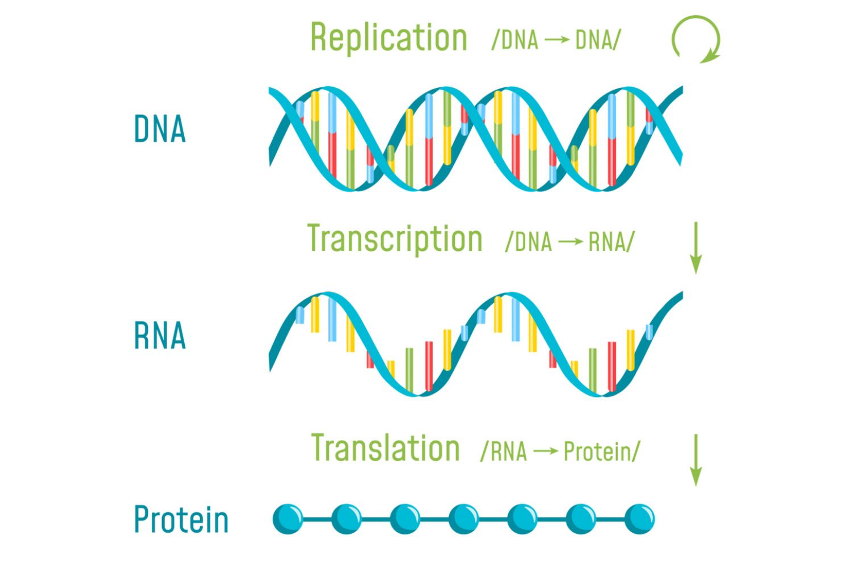
\includegraphics[width=0.5\linewidth]{\toplevelprefix/chapters/chapter1/figs/DNAs.png}
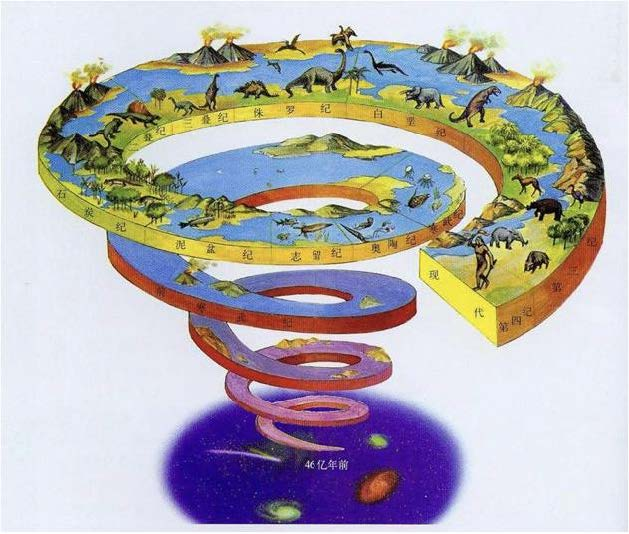
\includegraphics[width=0.40\linewidth]{\toplevelprefix/chapters/chapter1/figs/Evolution.jpg}
    \caption{Evoluția inteligenței filogenetice: Cunoașterea lumii externe este codată și transmisă prin ADN (stânga) și este decodată din ADN în ARN și în proteine etc. În stadiul timpuriu al evoluției vieții (dreapta), inteligența dezvoltă cunoștințe la nivel de specie prin mutația (aleatorie) a genelor și selecția naturală -- „fie ca cel mai apt să supraviețuiască", care poate fi văzută ca o formă primitivă de învățare prin întărire.}
    \label{fig:phylogenetic}
\end{figure}
\begin{figure}
    \centering
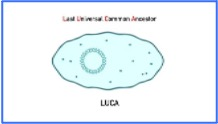
\includegraphics[height=0.19\linewidth]{\toplevelprefix/chapters/chapter1/figs/Luca.jpeg}
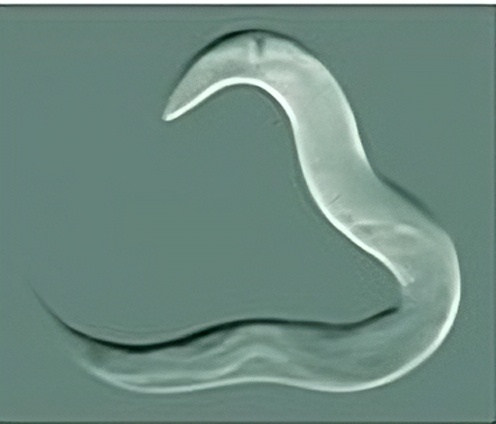
\includegraphics[height=0.19\linewidth]{\toplevelprefix/chapters/chapter1/figs/Worm.jpeg}
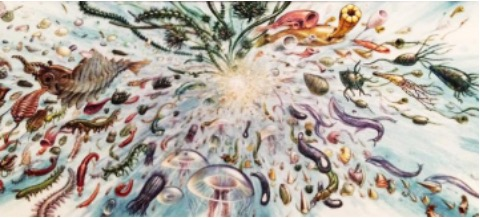
\includegraphics[height=0.19\linewidth]{\toplevelprefix/chapters/chapter1/figs/Cambrian.jpg}
    \caption{Evoluția vieții, de la strămoșul întregii vieți de astăzi (numit LUCA --- ultimul strămoș comun universal), un organism asemănător unei celule unice care a trăit acum 3,5-4,3 miliarde de ani, la apariția primului sistem nervos în specii asemănătoare viermilor (mijloc), acum aproximativ 550 de milioane de ani, la explozia formelor de viață în perioada cambriană (dreapta), acum aproximativ 530 de milioane de ani.}
    \label{fig:evolution}
\end{figure}

{\em Inteligența ontogenetică} se referă la mecanismele de învățare care permit unui individ să învețe prin propriile simțuri, amintiri și predicții în cadrul mediului său specific de viață și să-și îmbunătățească și adapteze comportamentele. Învățarea ontogenetică a devenit posibilă după apariția sistemului nervos acum aproximativ 550-600 de milioane de ani (în organisme asemănătoare viermilor), prezentată în \Cref{fig:evolution} mijloc. Adică, cu un sistem senzorial și nervos, un individ este capabil să formeze și să-și îmbunătățească continuu propriile cunoștințe despre lume, cunoscute și sub numele de memorie, pe lângă ceea ce este moștenit din ADN-ul sau genele sale. Această capacitate a îmbunătățit semnificativ supraviețuirea individului și a contribuit la explozia formelor de viață în perioada cambriană de acum aproximativ 530 de milioane de ani. Comparativ cu învățarea filogenetică, învățarea ontogenetică este semnificativ mai eficientă și previzibilă, care poate fi realizată în limitele de resurse ale unui individ în durata sa de viață.

Observați că ambele tipuri de mecanisme de învățare se bazează pe o formă de feedback (din mediul extern), în termeni de pedeapsă (moarte) sau recompensă (hrană), a acțiunilor unei specii sau ale indivizilor\footnote{Mutația genelor speciei sau acțiunile făcute de individ.} pentru a învăța. Ca rezultat, toate ființele inteligente, ca specii sau ca indivizi, se bazează pe un mecanism de feedback în buclă închisă pentru a învăța și a-și îmbunătăți cunoștințele despre lume. Observăm, de asemenea, că de la plante, la pești, la păsări și la mamifere, speciile mai avansate se bazează din ce în ce mai mult pe capacitățile lor de învățare ontogenetică. Ei stau cu părinții lor și învață de la ei din ce în ce mai mult după naștere, deoarece indivizii din aceeași specie trebuie să supraviețuiască în medii foarte diverse.

\paragraph{Evoluția inteligenței umane.}
De la apariția homo sapiens acum aproximativ 315 mii de ani, a apărut o formă nouă și superioară de inteligență care evoluează mai eficient și economic. Limbajele, mai întâi vorbite și apoi scrise\footnote{Limba sumeriană este considerată a fi una dintre cele mai vechi limbi scrise existente, atestată pentru prima dată în jurul anului 3100 î.Hr. în sudul Mesopotamiei.}, au fost dezvoltate acum câteva mii de ani. Vezi \Cref{fig:human-intelligence}. Aceasta permite indivizilor să comunice și să împărtășească informații utile cu alții. Prin urmare, o comunitate sau societate umană se poate comporta ca un singur organism inteligent care poate învăța mult mai repede și poate deține mai multe cunoștințe decât orice individ. Într-un fel, limbajele scrise, sau textele, joacă un rol similar cu ADN-ul și genele, deoarece permit societăților umane să acumuleze și să transmită cunoștințe despre lume generațiilor următoare. Ne putem referi la acest tip de inteligență ca {\em inteligență societală}, pentru a o distinge de inteligența filogenetică a speciilor și inteligența ontogenetică a indivizilor. Acest tip de acumulare de cunoștințe servește drept fundație a civilizațiilor antice.
\begin{figure}
    \centering
    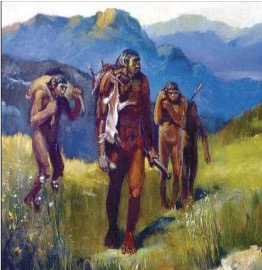
\includegraphics[height=0.25\linewidth]{\toplevelprefix/chapters/chapter1/figs/Spoken-language.jpg}
   \hspace{5mm} 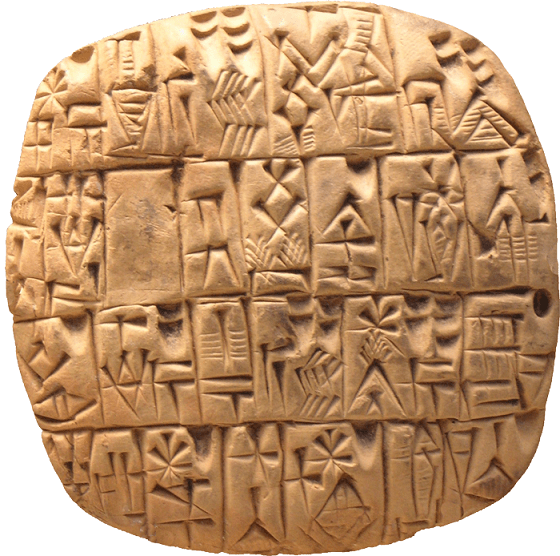
\includegraphics[height=0.25\linewidth]{\toplevelprefix/chapters/chapter1/figs/Cuneiform.png}
   \hspace{5mm} 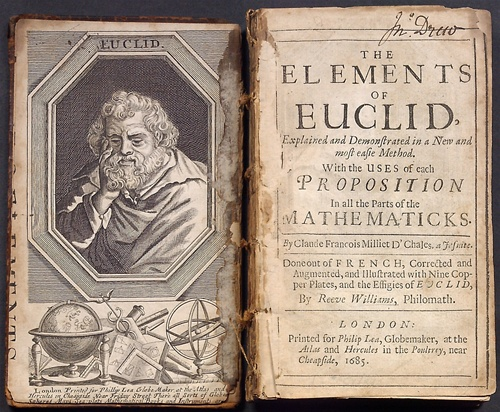
\includegraphics[height=0.25\linewidth]{\toplevelprefix/chapters/chapter1/figs/adopt-euclid1685-2.jpg}
    \caption{Dezvoltarea comunicării verbale și a limbajelor vorbite (între 10000-5000 î.Hr.), a limbajelor scrise (aproximativ 3000 î.Hr.) și a matematicii (în jurul anilor 500-300 î.Hr.) marchează trei repere cheie în evoluția inteligenței umane.}
    \label{fig:human-intelligence}
\end{figure}

Destul de miraculos, acum câteva mii de ani, a avut loc un alt salt cuantic în inteligența umană, care le-a permis filozofilor și matematicienilor să dezvolte cunoștințe care par să depășească cu mult dezvoltarea cunoștințelor empirice. Dezvoltarea conceptelor și simbolurilor matematice abstracte, cum ar fi numerele, spațiul și timpul, precum și logica matematică, servesc ca un nou limbaj precis pentru știința modernă. În plus, dezvoltarea abilității de a genera noi ipoteze și de a verifica corectitudinea acestora pe baza deducției logice sau a experimentării științifice. Aceasta, pentru prima dată, a permis oamenilor să dezvolte proactiv cunoștințe noi dincolo de mijloacele empirice pasive. Se crede că abilitatea de a desfășura aceste forme de dezvoltare a cunoștințelor de nivel înalt este unică pentru oameni. Această formă avansată de inteligență este denumită „inteligență artificială" (AI), termen inventat de John McCarthy la atelierul de vară de la Dartmouth din 1956.

Prin urmare, din ceea ce putem învăța din natură, de acum înainte, ori de câte ori folosim cuvântul „inteligență", trebuie să fim foarte specifici despre ce nivel/formă de inteligență ne referim:
\begin{equation}
\mbox{\textbf{filogenetică}} \;
   \Longrightarrow \; \mbox{\textbf{ontogenetică}} \; \Longrightarrow \;
   \mbox{\textbf{societală}}
   \; \Longrightarrow \;
   \mbox{\textbf{inteligență artificială}}.
\end{equation}
O caracterizare și distincție clară sunt necesare și importante deoarece vrem să studiem inteligența ca subiect științific și matematic. Este foarte probabil că, chiar dacă toate pot împărtăși obiectivul comun de a învăța cunoștințe utile despre lume, mecanismele computaționale specifice și implementările fizice din spatele fiecărui nivel/formă de inteligență ar putea fi diferite. Credem că cititorul va înțelege și aprecia mai bine aceste diferențe după ce va termina de studiat această carte. Prin urmare, vom lăsa mai multe discuții despre inteligența generală pentru ultimul \Cref{ch:future}.




\paragraph{Originea inteligenței mașinilor -- Cibernetica.}
În anii 1940, parțial din cauza efortului de război, inteligența din natură a inspirat oamenii de știință să emuleze inteligența animalelor prin mașini, ceea ce a dus la mișcarea „Cibernetică" promovată de Norbert Wiener. Wiener a studiat zoologia la Harvard ca student, dar mai târziu a devenit matematician și teoretician al controlului. Wiener a avut o pasiune pe viață pentru înțelegerea și dezvoltarea sistemelor autonome care ar putea emula comportamentele inteligente ale animalelor. Astăzi, programul Cibernetică este adesea interpretat îngust de oameni ca fiind în principal despre sistemele de control cu feedback pentru care Wiener a făcut într-adevăr cele mai semnificative contribuții tehnice. Dar programul Cibernetică a fost mult mai larg și mai profund decât atât. Este mai mult despre înțelegerea inteligenței ca întreg\footnote{Cel puțin la nivelul animalelor.} și a influențat de fapt munca unei întregi generații de oameni de știință renumiți, inclusiv Warren McCulloch, Walter Pitts, Claude Shannon, John von Neumann și Alan Turing.

\begin{figure}
    \centering
    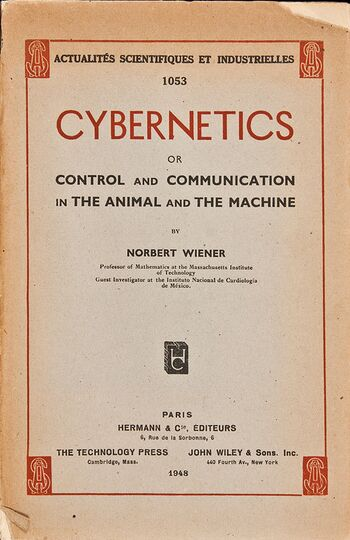
\includegraphics[height=0.4\linewidth]{\toplevelprefix/chapters/chapter1/figs/Cybernetics1.jpg}
    \hspace{10mm} 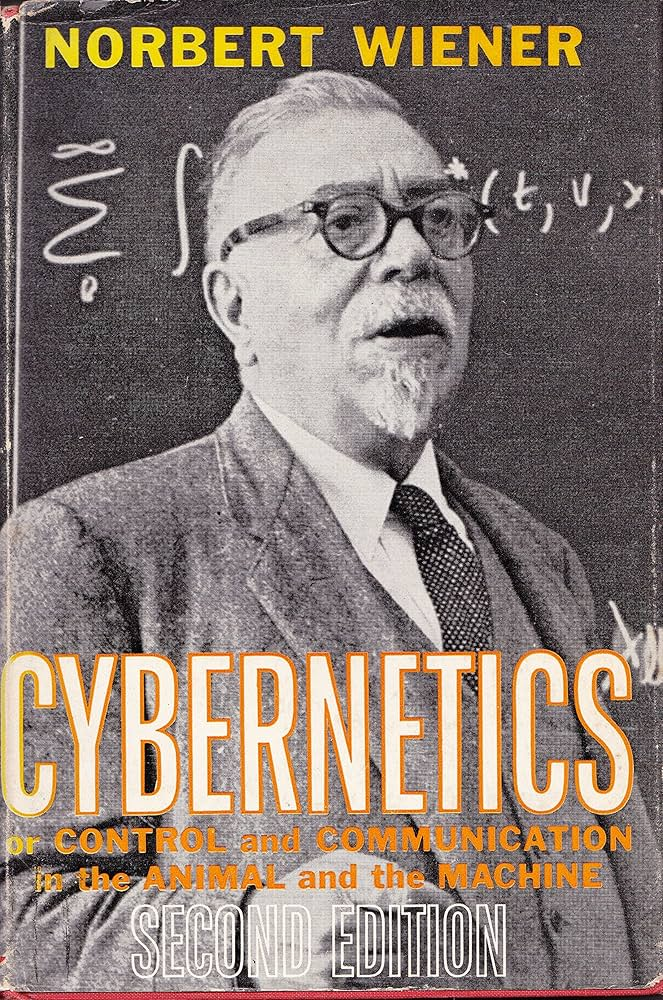
\includegraphics[height=0.4\linewidth]{\toplevelprefix/chapters/chapter1/figs/Cybernetics2.jpg}
    \caption{Cartea „Cibernetica" de Norbert Wiener publicată în 1948 \cite{Wiener-Cybernetics-1948} (stânga) și a doua ediție în 1961 \cite{Wiener-Cybernetics-1961} (dreapta).}
    \label{fig:cybernetcis}
\end{figure}


Wiener a fost probabil prima persoană care a studiat inteligența ca {\em un sistem}, în loc să acorde atenție doar unei componente sau aspect al acesteia. Viziunile sale cuprinzătoare asupra inteligenței au fost elaborate în faimoasa sa carte din 1948 {\em „Cibernetica: sau Control și Comunicare în Animal și Mașină"} \cite{Wiener-Cybernetics-1948}. În această carte și în a doua ediție publicată în 1961 \cite{Wiener-Cybernetics-1961} (vezi \Cref{fig:cybernetcis}), el a încercat să identifice mai multe caracteristici și mecanisme necesare ale sistemelor inteligente, care includ (dar nu se limitează la):
\begin{itemize}
    \item Cum să {\em măsurăm și stocăm} informația (în creier) și cum să comunicăm cu alții.\footnote{Norbert Wiener a fost primul care a subliniat că „informația" nu este materie sau energie, ci o cantitate independentă pentru studiu.} Aceasta a dus la formularea teoriei informației și teoriei codării de către Claude Shannon în 1948.
    \item Cum să {\em corectăm erorile} în predicție și estimare pe baza informațiilor existente. Norbert Wiener însuși a ajutat la formalizarea teoriei pentru sistemele de control bazate pe feedback în buclă închisă în anii 1940.
    \item Cum să învățăm să {\em luăm decizii mai bune} din interacțiunea cu un oponent potențial necooperant sau un mediu adversarial. Aceasta a fost formalizată de John von Neumann ca teoria jocurilor în 1944.
\end{itemize}
În 1943, foarte motivat de programul Cibernetică al lui Wiener, psihiatrul Warren McCulloch și logicianul Walter Pitts au formalizat împreună primul model computațional pentru un neuron \cite{McCulloch-Pitts}, numit {\em un neuron artificial}, așa cum este ilustrat mai târziu în \Cref{fig:neuron}. Bazat pe acest model, în anii 1950, Frank Rosenblatt a construit o mașină fizică, numită {\em Mark I Perceptron}, cu o rețea de sute de astfel de neuroni artificiali. Perceptron a fost prima rețea neuronală artificială realizată fizic, vezi \Cref{fig:perceptron}. În mod notabil, arhitectura computerului universal a lui John von Neumann, propusă în 1945, a fost de asemenea concepută pentru a facilita obiectivul de a construi {\em mașini de calcul} care pot realiza fizic mecanismele sugerate de programul Cibernetică.

Cititorii atenți probabil au observat că anii 1940 au fost cu adevărat o epocă magică: Atât de multe idei fundamentale au fost inventate și teorii influente formalizate în acea epocă, inclusiv modelul matematic al neuronilor, rețelele neuronale artificiale, teoria informației, teoria controlului, teoria jocurilor și mașinile de calcul. \Cref{fig:god-fathers} arată câțiva dintre pionierii acestor teorii. După cum știm acum, fiecare lucrare de mai sus a crescut pentru a deveni fundamentul unui domeniu științific sau ingineresc pentru următoarele decenii și are un impact extraordinar asupra noastră. Toate aceste teorii fundamentale au fost inspirate și motivate de obiectivul de a încerca să dezvolte mașini care pot emula inteligența din natură. Pe baza notelor istorice, mișcarea Cibernetică a lui Wiener a influențat aproape toți acești oameni și muncă. Într-o mare măsură, programul Cibernetică stabilit de Wiener poate fi văzut ca adevăratul predecesor al programului foarte popular în prezent de inteligență „încorporată". De fapt, Wiener a descris programul în termeni mult mai concreți \cite{Wiener-Cybernetics-1961}.
\begin{figure}
    \centering
    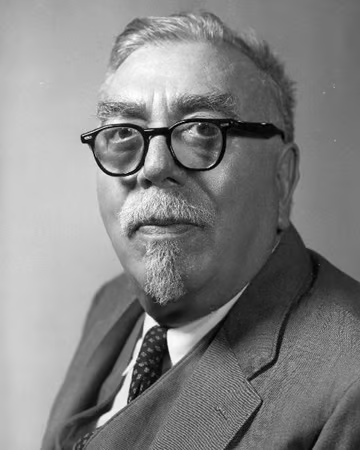
\includegraphics[height=0.3\linewidth]{\toplevelprefix/chapters/chapter1/figs/Wiener.png}
    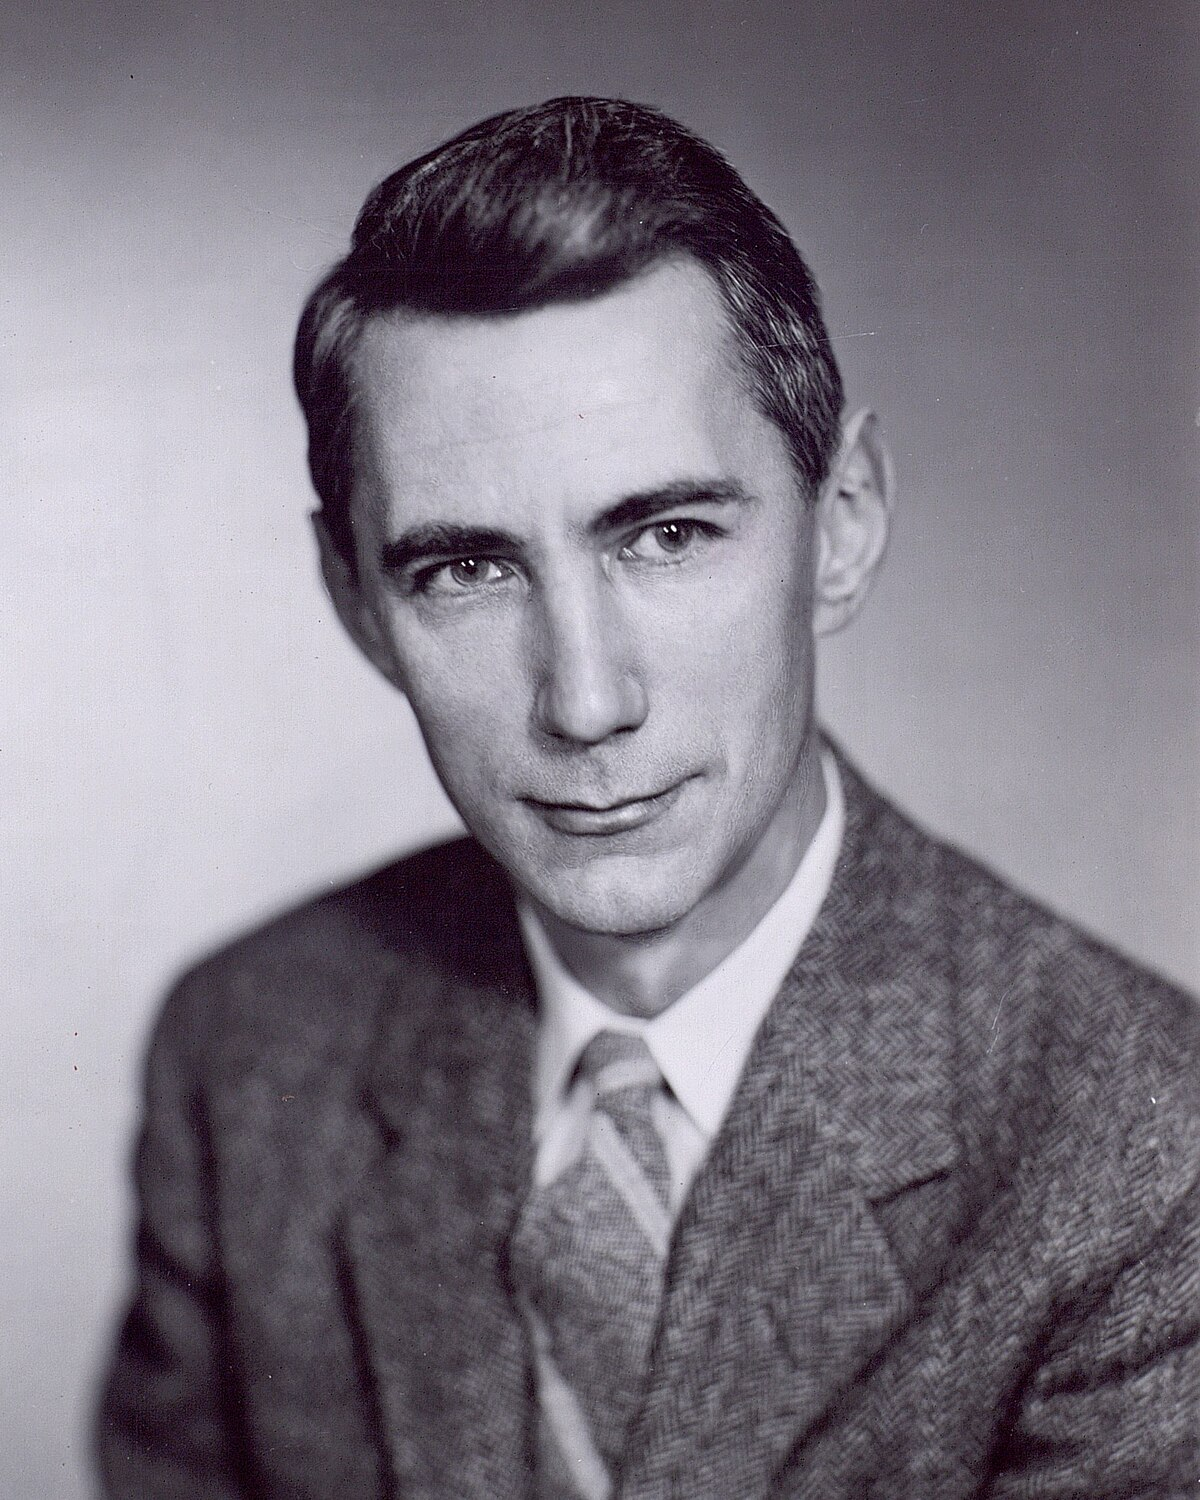
\includegraphics[height=0.3\linewidth]{\toplevelprefix/chapters/chapter1/figs/Shannon.jpg}
    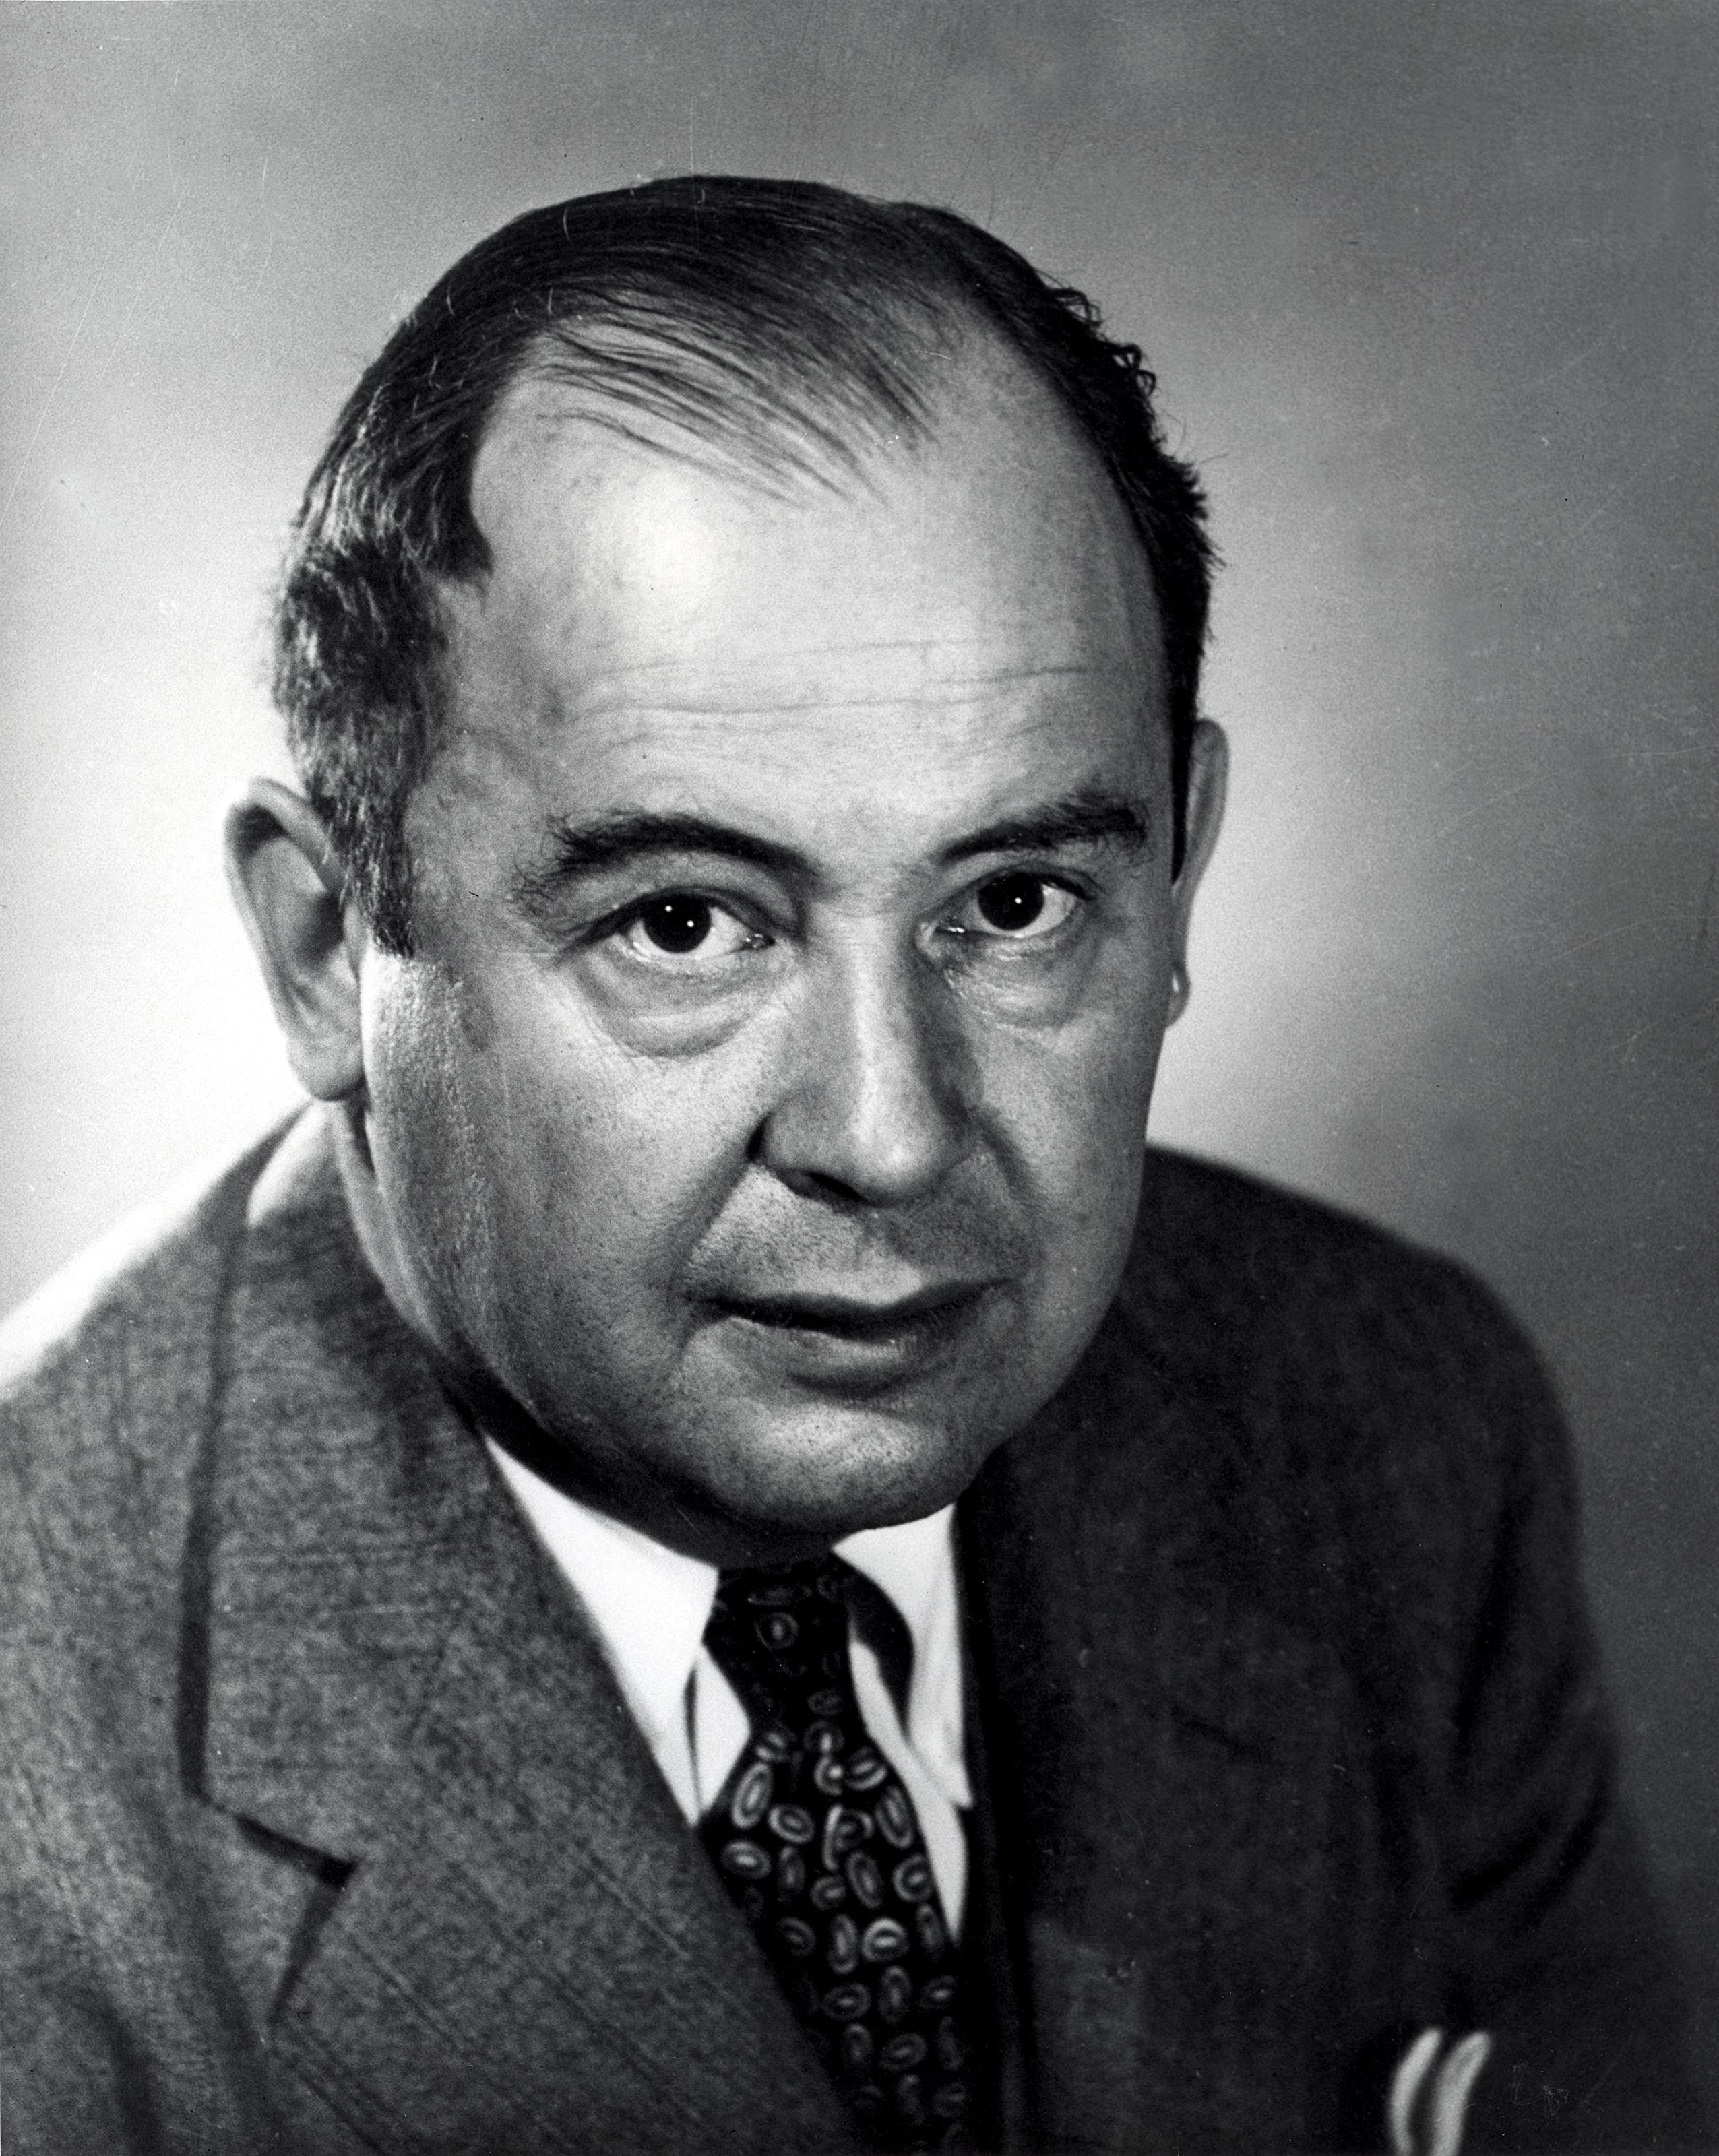
\includegraphics[height=0.3\linewidth]{\toplevelprefix/chapters/chapter1/figs/neumann.jpg}
    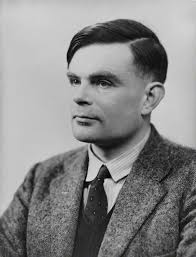
\includegraphics[height=0.3\linewidth]{\toplevelprefix/chapters/chapter1/figs/Turing.jpeg}
    \caption{Pionierii fundamentelor teoretice și computaționale pentru inteligență: Norbert Wiener (cibernetică și teoria controlului), Claude Shannon (teoria informației), John von Neumann (teoria jocurilor) și Alan Turing (teoria calculului).}
    \label{fig:god-fathers}
\end{figure}

Deși Wiener a identificat în munca sa multe caracteristici și mecanisme cheie ale inteligenței (încorporate), nu există nicio indicație că știa cum să integreze corespunzător toate aceste mecanisme împreună pentru a construi un sistem inteligent autonom complet. Judecând după cunoștințele de astăzi, unele dintre opiniile sale despre aceste mecanisme nu au fost în întregime corecte sau complete. În special, în ultimul capitol al celei de-a doua ediții a Ciberneticii \cite{Wiener-Cybernetics-1961}, el a subliniat că este crucial să {\em abordăm neliniaritatea} dacă un sistem de învățare automată este conceput pentru a emula mecanismele tipice de învățare din natură. Dar el nu a oferit soluții concrete și eficiente la această problemă dificilă. În apărarea sa însă, la acea vreme, puțini oameni știau cum, deoarece chiar și teoria pentru abordarea modelelor și sistemelor liniare era încă în stadiul incipient.

Cu toate acestea, nu ne-am putut abține să nu ne minunăm de previziunea lui Wiener despre importanța neliniarității. După cum vom vedea în această carte, răspunsul a fost găsit doar recent: neliniaritatea poate fi abordată eficient prin linearizare progresivă și transformare realizată de rețele neuronale profunde (vezi \Cref{ch:representation}). În plus, vom încerca să arătăm în această carte cum toate aceste mecanisme enumerate mai sus pot fi integrate natural într-un sistem complet care ar prezenta caracteristicile unui sistem inteligent autonom (vezi \Cref{ch:autoencoding}).

\paragraph{Originea Inteligenței Artificiale.}
Din subtitlul cărții Cibernetica lui Wiener: {\em „Control și Comunicare în Animal și Mașină"}, se poate spune că studiile din anii 1940 au vizat în principal emularea inteligenței la nivelul animalelor. După cum am menționat înainte, agendele de cercetare despre inteligență din jurul anilor 1940 au fost foarte mult dominate de mișcarea Cibernetică a lui Norbert Wiener.

Alan Turing a fost unul dintre primii care a observat această limitare. În celebra sa lucrare din 1950 „{\em Mașini de Calcul și Inteligență}" \cite{Turing-1950}, Turing a pus oficial întrebarea dacă mașinile pot imita inteligența chiar și la nivel uman, până la punctul de a fi indistinguibile de capacitățile inteligente ale oamenilor. Aceasta este acum cunoscută sub numele de {\em testul Turing}.

În jurul anului 1955, un grup de oameni de știință tineri și ambițioși au încercat să se desprindă de mișcarea și agendele de cercetare dominante ale Ciberneticii, astfel încât să aibă șansa de a-și crea propria moștenire. Au decis să accepte provocarea lui Turing de a imita inteligența umană și au propus un atelier care să aibă loc la Dartmouth College în vara anului 1956. Și-au făcut intenția clară cu o declarație în propunerea lor:
\begin{quote}
    „{\em Studiul urmează să procedeze pe baza conjecturii că fiecare aspect al învățării sau orice altă caracteristică a inteligenței poate fi în principiu descris atât de precis încât o mașină poate fi făcută să-l simuleze. Se va încerca să se găsească cum să facem mașinile să folosească limbajul, să formeze abstracții și concepte, să rezolve tipuri de probleme acum rezervate oamenilor și să se îmbunătățească}."
\end{quote}
În esență, ei au vrut să formalizeze și să studieze inteligența de nivel superior care diferențiază oamenii de animale. Subiectele pe care le-au luat în considerare au variat de la abstracție, metode simbolice, limbaje naturale și metode deductive (inclusiv inferență cauzală, deducție logică etc.) Organizatorul atelierului, John McCarthy, pe atunci un tânăr profesor asistent de matematică la Dartmouth College, a inventat termenul acum faimos „Inteligență Artificială" (AI) pentru a încapsula setul de caracteristici sau mecanisme care se crede că sunt {\em unice pentru inteligența umană}.

\paragraph{Renașterea „Inteligenței Artificiale" sau a „Ciberneticii"?}
După cum cititorii ar putea ști, în ultimul deceniu sau cam așa ceva, inteligența mașinilor a suferit o dezvoltare explozivă, alimentată în principal de practica rețelelor neuronale artificiale profunde, declanșată de munca lui Geoffrey Hinton și studenții în 2012 \cite{krizhevsky2012imagenet}. Această eră este de asemenea salutată ca „Renașterea" Inteligenței Artificiale (AI). Cu toate acestea, în ceea ce privește sarcinile pe care oamenii au încercat de fapt să le abordeze (recunoaștere, generare și predicție) și tehnicile pe care oamenii le-au dezvoltat și implementat până acum (întărire, imitare, codare, decodare, îndepărtarea zgomotului și compresie), emulăm foarte mult doar mecanismele care sunt comune inteligenței vieții timpurii și animalelor. Chiar și în această privință, după cum vom încerca să clarificăm în această carte, modelele și sistemele „AI" actuale nu au implementat corect toate mecanismele necesare pentru inteligența la aceste niveluri, care erau deja cunoscute mișcării Cibernetice din anii 1940.

Prin urmare, strict vorbind, avansul inteligenței mașinilor din ultimul deceniu nu se aliniază bine cu programul „Inteligență Artificială" stabilit în atelierul de la Dartmouth din 1956. În schimb, ceea ce a fost realizat predominant până acum este mai strâns legat de obiectivele programului clasic „Cibernetică" stabilit de Norbert Wiener în anii 1940. Probabil este mai potrivit să numim epoca actuală „Renașterea Ciberneticii".\footnote{Creșterea recentă a așa-numitei „AI Încorporate" pentru roboți inteligenți autonomi împărtășește și mai multă similitudine cu obiectivele programului Cibernetică.} Doar după ce am înțeles pe deplin ceea ce am făcut cu adevărat din perspectiva științifică și matematică, putem ști cu adevărat ce rămâne de făcut și în ce direcție să mergem pentru a urmări adevărata natură a inteligenței. Acesta este unul dintre scopurile principale ale acestei cărți.


\section{Ce să Învățăm?}
\label{sec:what-to-learn}



\subsection{Predictibilitate}
\label{sec:predictability}
Datele care poartă informații utile se manifestă în multe forme diferite. În forma cea mai naturală, ele pot fi modelate ca secvențe care sunt previzibile și calculabile. Noțiunea și proprietățile unei secvențe previzibile și calculabile au fost în centrul teoriei calculului și au dus în mare parte la inventarea calculatoarelor \cite{Turing-1936}. Rolul secvențelor previzibile în inferența (inductivă) a fost studiat de Ray Solomonoff, Andrey Kolmogorov și mulți alții în anii 1960 \cite{Kolmogorov1998OnTO} ca o generalizare a Teoriei Informației clasice a lui Claude Shannon \cite{Shannon-1948}. Pentru a înțelege conceptul de secvențe previzibile, să începem mai întâi cu câteva exemple concrete simple.
\paragraph{Cazul Scalar.} Cea mai simplă secvență discretă previzibilă este probabil secvența numerelor naturale:
\begin{equation}
   {S} =  1, 2, 3, 4, 5, 6, \ldots, n, n+1, \ldots
\end{equation}
în care următorul număr $x_{n+1}$ este definit ca numărul său anterior $x_n$ plus 1:
\begin{equation}
x_{n+1} = x_n + 1.
\end{equation}
Se poate generaliza noțiunea de predictibilitate la orice secvență $\{x_n\}_{n=1}^\infty$ cu $ x_n \in \mathbb{R}$ dacă următorul număr $x_{n+1}$ poate fi întotdeauna calculat din cel anterior $x_n$:
\begin{equation}
    x_{n+1} = f(x_{n}), \quad x_n \in \mathbb{R}, \; n =  1, 2, 3, \ldots
\end{equation}
unde $f(\cdot)$ este o funcție {\em calculabilă} (scalară).\footnote{Aici subliniem că funcția $f(\cdot)$ însăși este calculabilă, ceea ce înseamnă că poate fi implementată ca un program pe un computer.} Notați că aici subliniem că funcția $f(\cdot)$ trebuie să fie calculabilă. Există multe funcții care pot fi definite dar nu sunt calculabile. Lucrarea seminală a lui Alan Turing din 1936 \cite{Turing-1936} oferă o definiție riguroasă a calculabilității. În practică, adesea presupunem în plus că $f$ este calculabilă eficient și are proprietăți frumoase cum ar fi fiind continuă și diferențiabilă etc. Necesitatea acestor proprietăți va deveni clară mai târziu odată ce înțelegem mai multe despre noțiuni mai rafinate de calculabilitate și rolurile lor în învățarea automată și inteligență.

\paragraph{Cazul Multi-Variabil.}
Desigur, valoarea următorului număr poate depinde și de doi dintre predecesorii săi. De exemplu, faimoasa {\em secvență Fibonacci} este definită ca:
\begin{equation}
    {S} = 1, 1, 2, 3, 5, 8, 13, 21, 34, 55, \ldots
\end{equation}
unde se poate vedea ușor:
\begin{equation}
    x_{n+2} = x_{n+1} + x_{n}, \quad  x_n \in \mathbb{R}, \;  n = 1, 2, 3, \ldots
\end{equation}
În mod similar, putem generaliza această recursiune la \begin{equation}
    x_{n+2} = f(x_{n+1}, x_{n}), \quad x_n \in \mathbb{R}, \;  n =  1, 2, 3, \ldots
\end{equation}
unde $f(\cdot,\cdot)$ este orice funcție calculabilă care ia două variabile ca intrare. Putem generaliza în continuare noțiunea de predictibilitate la o secvență a cărei valoare următoare depinde de, să zicem, $d$ dintre predecesorii săi:
\begin{equation}
    x_{n+d} = f(x_{n+d-1}, \ldots,  x_{n}), \quad  x_n \in \mathbb{R}, \; n =  1, 2, 3, \ldots
    \label{eqn:recursive-d}
\end{equation}
Numărul de predecesori $d$ necesari pentru predicție se numește {\em gradul} predicției recursive. Expresia de mai sus \eqref{eqn:recursive-d} se mai numește și {\em (auto) regresie}. O astfel de secvență se mai numește și secvență {\em auto-regresivă}. Dacă funcția $f$ este o funcție liniară, o numim regresie (auto) liniară.

\paragraph{Cazul Vectorial.}
Pentru a simplifica notația, putem defini un vector $\vx \in \mathbb{R}^d$ care colectează $d$ valori consecutive în secvență: \begin{equation}
    \vx_n \doteq [x_{n+d-1}, \ldots,  x_{n}]^\top, \quad \vx_n \in \mathbb{R}^d, \; n = 1, 2, 3, \ldots
\end{equation}
Cu această notație, relația recursivă \eqref{eqn:recursive-d} poate fi scrisă convenabil ca
\begin{equation}
    \vx_{n+1} = g(\vx_{n}) \; \in \mathbb{R}^d, \quad n =  1, 2, 3, \ldots
    \label{eqn:recursive-v}
\end{equation}
unde funcția $g(\cdot)$ este definită unic de funcția $f$ în \eqref{eqn:recursive-d} și ia un vector $d$-dimensional ca intrare. În contexte diferite, un astfel de vector este uneori denumit „stare" sau „token". Notați că ecuația din \eqref{eqn:recursive-d} denotă o mapare $\mathbb{R}^d \rightarrow \mathbb{R}$, dar ecuația de aici este $g: \mathbb{R}^d \rightarrow \mathbb{R}^d$.


\paragraph{Predicție Controlată.}
Putem defini, de asemenea, o secvență previzibilă care depinde de o altă secvență previzibilă ca intrare:
\begin{equation}
    \vx_{n+1} = f(\vx_{n}, \vu_n) \; \in \mathbb{R}^d, \quad n =  1, 2, 3, \ldots,
\label{eqn:recursive-control}
\end{equation}
unde $\{\vu_n\}$ cu $\vu_n \in \mathbb{R}^k$ este o secvență previzibilă (calculabilă). Cu alte cuvinte, următorul vector $\vx_{n+1} \in \mathbb{R}^d$ depinde atât de $\vx_n \in \mathbb{R}^d$ cât și de $\vu_n \in \mathbb{R}^k$. În contextul teoriei controlului, secvența $\{\vu_n\}$ este adesea denumită „intrarea de control" și $\vx_n$ ca „starea" sau „ieșirea" sistemului \eqref{eqn:recursive-control}. Un exemplu clasic este un sistem dinamic liniar:
\begin{equation}
    \vx_{n+1} = \boldsymbol{A}\vx_n + \boldsymbol{B}\vu_n, \quad \boldsymbol{A} \in \mathbb{R}^{d\times d}, \boldsymbol{B} \in \mathbb{R}^{d\times k},
    \label{eqn:lineary-system}
\end{equation}
care este studiat pe larg în teoria controlului \cite{Cal:Des}.

Foarte des intrarea de control este dată de o funcție calculabilă a stării $\vx_n$ însăși:
\begin{equation}
    \vu_n = h(\vx_n), \quad n =  1, 2, 3, \ldots
\end{equation}
Ca rezultat, secvența $\{\vx_n\}$ este dată prin compunerea celor două funcții calculabile $f$ și $h$ ca:
\begin{equation}
    \vx_{n+1} = f\big(\vx_{n}, h(\vx_n)\big), \quad n =  1, 2, 3, \ldots
    \label{eqn:recursive-closed-loop}
\end{equation}
În acest fel, secvența $\{\vx_n\}$ devine din nou o secvență previzibilă auto-regresivă. Când intrarea $\vu_n$ depinde de ieșirea $\vx_n$, spunem că secvența rezultată este produsă de un sistem „în buclă închisă" \eqref{eqn:recursive-closed-loop}. Deoarece sistemul în buclă închisă nu mai depinde de nicio intrare externă, spunem că un astfel de sistem a devenit {\em autonom}. Poate fi văzut ca un caz special de auto-regresie. De exemplu, dacă alegem în sistemul liniar de mai sus \eqref{eqn:lineary-system}, $\vu_n = \boldsymbol{F}\vx_n$, sistemul în buclă închisă devine
\begin{equation}
        \vx_{n+1} = \boldsymbol{A}\vx_n + \boldsymbol{B}\vu_n = \boldsymbol{A}\vx_n + \boldsymbol{B}\boldsymbol{F}\vx_n = (\boldsymbol{A}+ \boldsymbol{B}\boldsymbol{F})\vx_n,
    \label{eqn:lineary-system-closed}
\end{equation}
care este o auto-regresie liniară.



\paragraph{Procese Continue.}
Secvențele previzibile au corespondente naturale în cazul continuu. Ne putem referi la ele ca procese previzibile. Similar cu secvența numerelor naturale, cel mai simplu proces continuu previzibil este timpul însuși $x=t$.

Mai general, spunem că un proces, notat cu $\vx(t)$, este previzibil dacă în orice moment $t$, valoarea procesului la $t+\delta t$, unde $\delta t$ este un increment infinitezimal, este determinată de valoarea sa la $t$. De obicei, schimbarea în valoare $\delta \vx(t)$ este continuă și netedă. Deci $\delta \vx(t) = \vx(t + \delta t) - \vx(t)$ este infinitezimal de mică. Procesele previzibile sunt de obicei descrise de ecuații diferențiale (multivariabile):
\begin{equation}
    \dot{\vx}(t) = f(\vx(t)), \quad \vx \in \mathbb{R}^d.
    \label{eqn:process}
\end{equation}

În contextul teoriei sistemelor \cite{Cal:Des,Sastry-Nonlinear}, ecuația de mai sus este cunoscută și ca model de spațiu de stare. Similar cu cazul discret, un proces controlat poate fi dat de:
\begin{equation}
    \dot{\vx}(t) = f(\vx(t), \vu(t) ), \quad \vx \in \mathbb{R}^d, \vu \in \mathbb{R}^k,
    \label{eqn:process-controlled}
\end{equation}
unde $\vu(t)$ este un proces de intrare calculabil.

\begin{example}
    De exemplu în fizică, a doua lege a mișcării a lui Newton descrie cum să prezicem traiectoria $\boldsymbol{x}(t) \in \mathbb{R}^3$ a unui obiect în mișcare sub o intrare de forță $\boldsymbol{F}(t) \in \mathbb{R}^3$:
\begin{equation}
    m\ddot{\boldsymbol{x}}(t) = \boldsymbol{F}(t).
\end{equation}
Când nu există forță $\boldsymbol{F}(t) \equiv 0$, legea de mai sus se reduce la un caz special, cunoscut ca prima lege a lui Newton: obiectul menține o viteză constantă în linie dreaptă:
\begin{equation}
   \ddot{\boldsymbol{x}}(t) = \boldsymbol{0} \; \Leftrightarrow \; \dot{\boldsymbol{x}}(t) = \boldsymbol{v}
\end{equation}
pentru un anumit vector de viteză constantă $\boldsymbol{v} \in \mathbb{R}^3$.
\end{example}




\subsection{Dimensionalitate Redusă}\label{sec:intro-low-dimensionality}
\paragraph{Învățarea Predicției.}
Acum să presupunem că ați observat sau vi s-au dat multe segmente de secvență:
\begin{equation}
    \{S_1, S_2, \ldots, S_i, \ldots, S_N\}
\end{equation}
toate dintr-o secvență previzibilă $\{x_n\}_{n=1}^\infty$. Fără pierderea generalității, putem presupune că lungimea fiecărui segment este $D \gg d$. Deci fiecare segment este de forma:
\begin{equation}
    S_i = [x_{j(i)}, x_{j(i)+1}, \ldots, x_{j(i)+D-1}]^\top \in \mathbb{R}^D
\end{equation}
pentru un anumit $j \in \mathbb{N}$. Apoi vi se dă un nou segment $S_t$ și vi se cere să preziceți valorile sale viitoare.

O dificultate aici este că în mod normal nu cunoașteți funcția $f$ și gradul $d$ din care este generată secvența:
\begin{equation}
    x_{n+d} = f(x_{n+d-1}, \ldots,  x_{n}).
\label{eqn:sequence-order-d}
\end{equation}
Deci speranța este cumva „să învățați" $f$ și $d$ din segmentele de eșantion date $S_1, S_2, \ldots, S_N$. Prin urmare, sarcina centrală a învățării predicției este:
\begin{center}
{\em Fiind date multe segmente eșantionate dintr-o secvență previzibilă, cum să identificăm eficient și eficace funcția $f$.}
\end{center}

\paragraph{Predictibilitate și Dimensionalitate Redusă.}
Pentru a identifica funcția predictivă $f$, putem observa o caracteristică comună a segmentelor oricărei secvențe previzibile date de \eqref{eqn:sequence-order-d}. Dacă luăm un segment lung, să zicem cu o lungime $D \gg d$, din secvență și îl privim ca un vector:
\begin{equation}
    \vx_i = [x_i, x_{i+1}, \ldots x_{i+D-1}]^\top \in \mathbb{R}^D.
\end{equation}
Atunci setul tuturor acestor vectori $\{\vx_i\}$ este departe de a fi aleatoriu și prin urmare nu poate ocupa întregul spațiu al $\R^D$. În schimb, ei au în esență cel mult $d$ grade de libertate -- date primele $d$ intrări ale oricărui $\vx_i$, valorile restului intrărilor sunt determinate unic. Cu alte cuvinte, toți $\{\vx_i\}$ se află pe o suprafață $d$-dimensională. În matematică, o astfel de suprafață este adesea numită o subvarietate, notată ca $\mathcal{S} \subset \R^D$.


\begin{figure}[t]
\centering
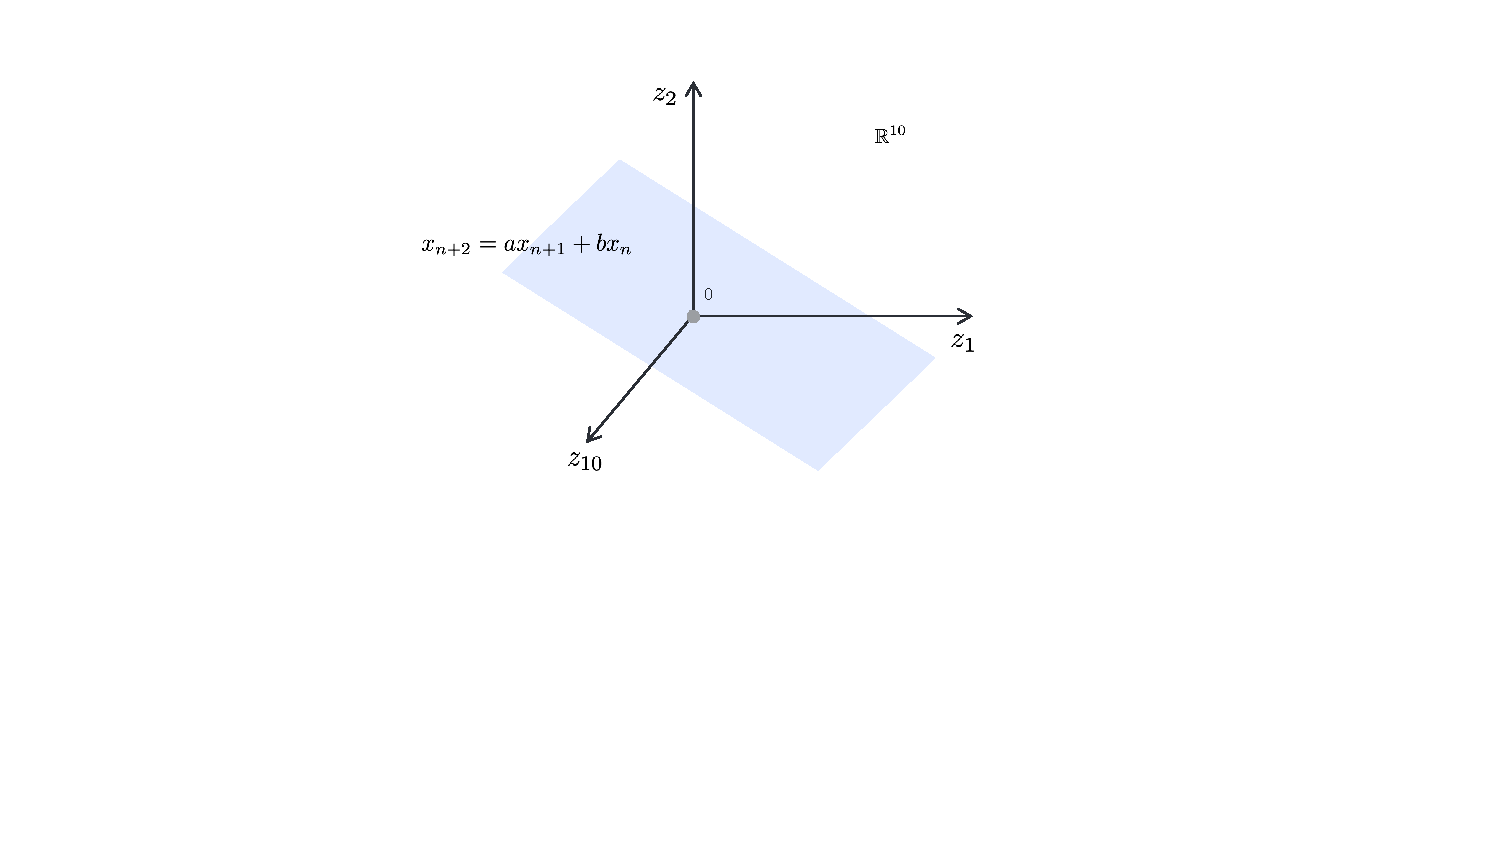
\includegraphics[width=0.6\linewidth]{\toplevelprefix/chapters/chapter1/figs/two-dimensional plane in R10.pdf}
    \caption{Un subspațiu bidimensional într-un spațiu ambiental zece-dimensional.}
    \label{fig:lowdimplane}
\end{figure}
În practică, dacă alegem lungimea segmentului $D$ să fie suficient de mare, atunci toate segmentele eșantionate din aceeași funcție de predicție se află pe o suprafață cu o dimensiune intrinsecă $d$, semnificativ mai mică decât cea a spațiului ambiental $D$. De exemplu, dacă secvența este dată de următoarea autoregresie liniară:
\begin{equation}
    x_{n+2} = a\cdot x_{n+1} + b\cdot x_n,
    \label{eqn:sequence-2d}
\end{equation}
pentru anumite constante $a, b \in \R$. Dacă eșantionăm segmente de lungime $D =10$ dintr-o astfel de secvență, atunci toate eșantioanele se află pe un plan sau subspațiu bidimensional în $\R^{10}$, așa cum este ilustrat în \Cref{fig:lowdimplane}. Dacă putem identifica acest subspațiu bidimensional, constantele $a$ și $b$ în \eqref{eqn:sequence-2d} pot fi determinate complet.


Este ușor de văzut că dacă funcția de predicție $f$ este liniară, cum ar fi cazul cu sistemele liniare date în \eqref{eqn:lineary-system} și \eqref{eqn:lineary-system-closed}, segmentele lungi se află întotdeauna pe un anumit subspațiu liniar cu dimensiuni reduse. Identificarea funcției de predicție este în mare măsură echivalentă cu identificarea acestui subspațiu cu dimensiuni reduse, o problemă cunoscută în general ca analiza componentelor principale. Vom discuta astfel de modele și metode clasice în \Cref{ch:classic}.

După cum se dovedește, acest lucru este în mare măsură adevărat și pentru secvențele previzibile generale: dacă cineva poate identifica suprafața cu dimensiuni reduse pe care se află toate eșantioanele de segmente, atunci poate identifica funcția predictivă asociată $f$.\footnote{În condiții blânde, există o mapare unu-la-unu între suprafața cu dimensiuni reduse și funcția $f$. Acest fapt a fost exploatat în probleme precum identificarea sistemului pe care o vom discuta mai târziu.} Nu putem sublinia suficient importanța acestei proprietăți a segmentelor dintr-o secvență previzibilă: {\em Toate eșantioanele de segmente lungi ale unei secvențe previzibile se află pe o subvarietate cu dimensiuni reduse.} După cum vom vedea în această carte, toate metodele moderne de învățare exploatează în esență această proprietate, implicit sau explicit.

În scenariile din lumea reală, datele pe care le observăm adesea nu provin dintr-o singură secvență previzibilă. De obicei, ele conțin observații ale mai multor secvențe previzibile. De exemplu, o secvență video poate conține mai multe obiecte în mișcare. Este ușor de văzut că în astfel de scenarii, datele se află pe un amestec de mai multe subspații liniare cu dimensiuni reduse sau subvarietăți neliniare, așa cum este ilustrat în \Cref{fig:mixture-models}.
\begin{figure}
    \centering
    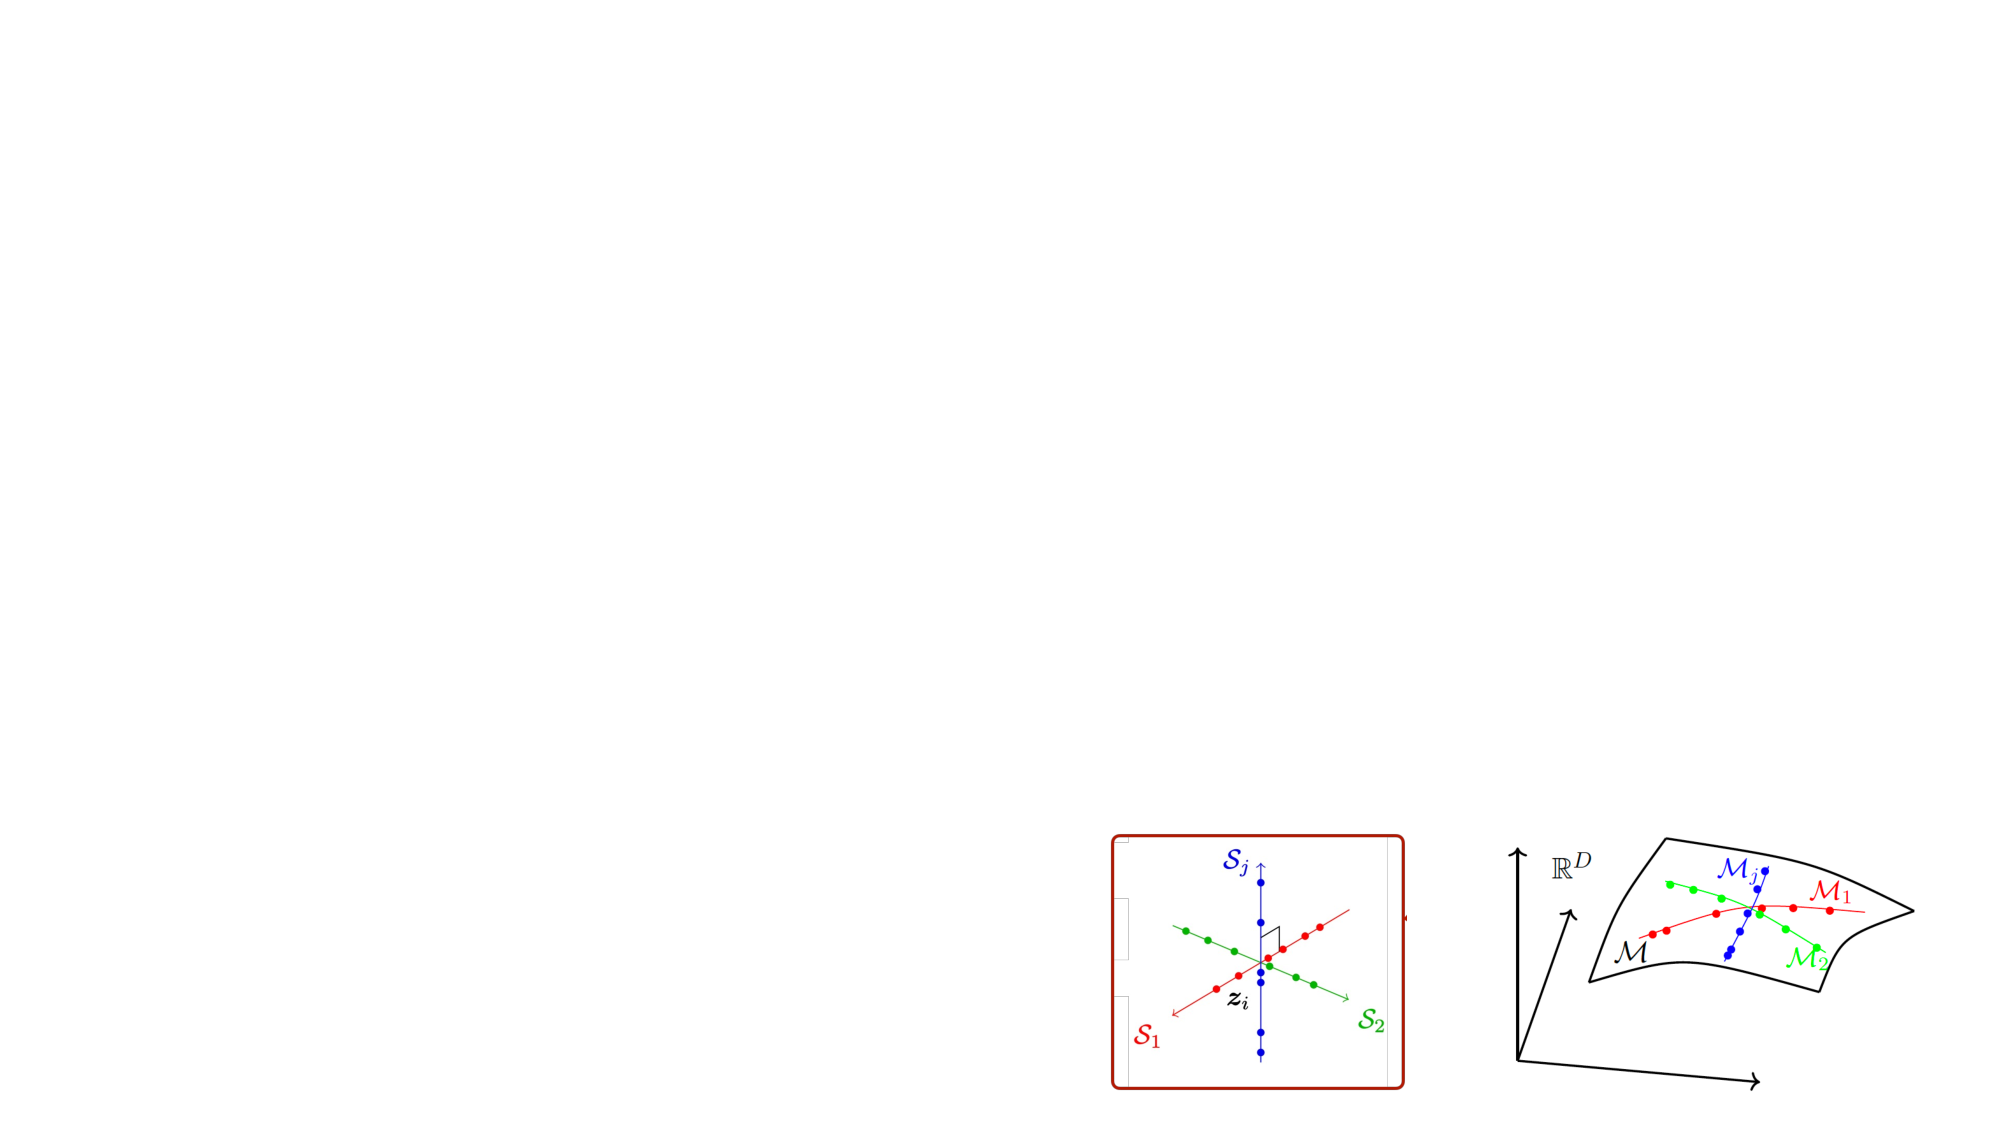
\includegraphics[width=0.8\linewidth]{\toplevelprefix/chapters/chapter1/figs/mixture.pdf}
    \caption{Date distribuite pe un amestec de subspații (ortogonale) (stânga) sau subvarietăți (dreapta).}
    \label{fig:mixture-models}
\end{figure}


\paragraph{Proprietățile Dimensionalității Reduse.}
Desigur, corelația temporală în secvențele previzibile nu este singurul motiv pentru care datele sunt cu dimensiuni reduse. De exemplu, spațiul tuturor imaginilor este imens, dar cea mai mare parte a spațiului constă din imagini care seamănă cu imagini aleatorii fără structură, așa cum se arată în \Cref{fig:noise-image} stânga. Cu toate acestea, imaginile și videoclipurile naturale sunt foarte redundante deoarece există o corelație spațială și temporală puternică între toate valorile pixelilor. Acesta este motivul pentru care putem recunoaște cu ușurință dacă o imagine este zgomotoasă sau curată, așa cum se arată în \Cref{fig:noise-image} mijloc și dreapta. Prin urmare, distribuția imaginilor naturale are o dimensiune intrinsecă foarte mică (în raport cu numărul total de pixeli ai unei imagini).

\begin{figure}
    \centering
    
\includegraphics[height=0.30\linewidth]{\toplevelprefix/chapters/chapter1/figs/Gaussian-noise.png}\hspace{2mm}
    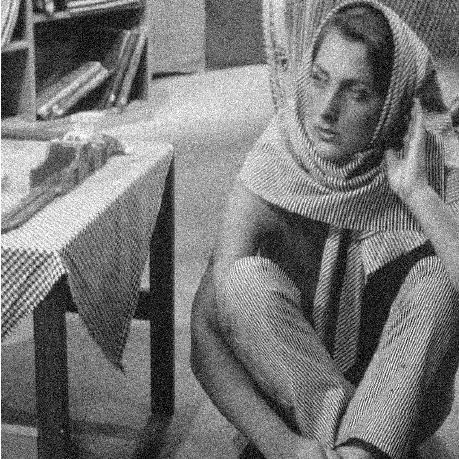
\includegraphics[height=0.30\linewidth]{\toplevelprefix/chapters/chapter1/figs/Standard-test-image-Barbara-of-size-512-512-pixels-including-Gaussian-noise-with.png} \hspace{2mm}
    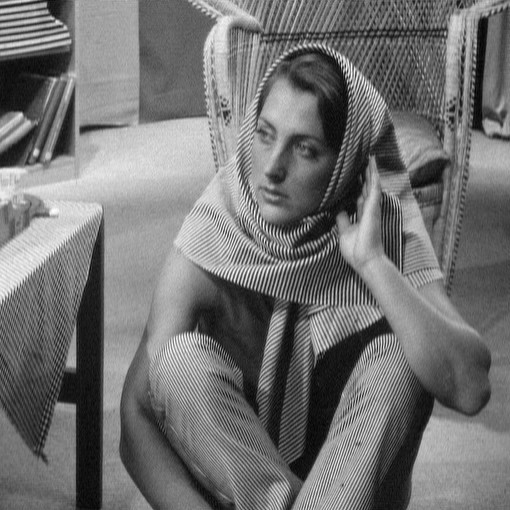
\includegraphics[height=0.30\linewidth]{\toplevelprefix/chapters/chapter1/figs/barbara.jpg}
    \caption{O imagine de zgomot aleatoriu versus o imagine zgomotoasă și imaginea originală curată.}
    \label{fig:noise-image}
\end{figure}

Datorită importanței și ubicuității sarcinii de învățare a structurilor cu dimensiuni reduse, cartea {\em „Analiza Datelor cu Dimensiuni Mari cu Modele cu Dimensiuni Reduse: Principii, Calcul și Aplicații"} \cite{Wright-Ma-2022} a declarat la început cu o afirmație: „{\em Problema identificării structurii cu dimensiuni reduse a semnalelor sau datelor în spații cu dimensiuni mari este una dintre cele mai fundamentale probleme care, printr-o istorie lungă, împletește multe domenii inginerești și matematice, cum ar fi teoria sistemelor, procesarea semnalelor, recunoașterea tiparelor, învățarea automată și statistica.}"

Notați că prin a forța punctul de date observat $\vx$ să fie pe o suprafață cu dimensiuni reduse, am făcut în esență intrările din $\vx$ foarte dependente una de alta și într-un anumit sens am făcut intrările foarte „previzibile" din valorile altor intrări. De exemplu, dacă știm că datele sunt constrânse pe o suprafață $d$-dimensională în $\R^D$, atunci ne permite să facem multe lucruri utile cu datele în afară de predicție:
\begin{itemize}
    \item \textbf{completare}: în general, date mai mult de $d$ intrări ale unui eșantion tipic $\vx$, restul intrărilor sale pot fi de obicei determinate {\em unic}.\footnote{Predicția devine un caz special al acestei proprietăți.}
    \item \textbf{îndepărtarea zgomotului}: să presupunem că intrările unui eșantion $\vx$ sunt perturbate de zgomote {\em mici}, ele pot fi îndepărtate eficient proiectând $\vx$ înapoi pe suprafață.
    \item \textbf{corectarea erorilor}: să presupunem că un număr mic de intrări {\em necunoscute} ale lui $\vx$ sunt corupte arbitrar, ele pot fi corectate eficient și eficace.
\end{itemize}
\Cref{fig:low-dim-properties} ilustrează aceste proprietăți cu o structură liniară cu dimensiuni reduse: o linie unidimensională într-un plan bidimensional.

\begin{figure}
    \centering
    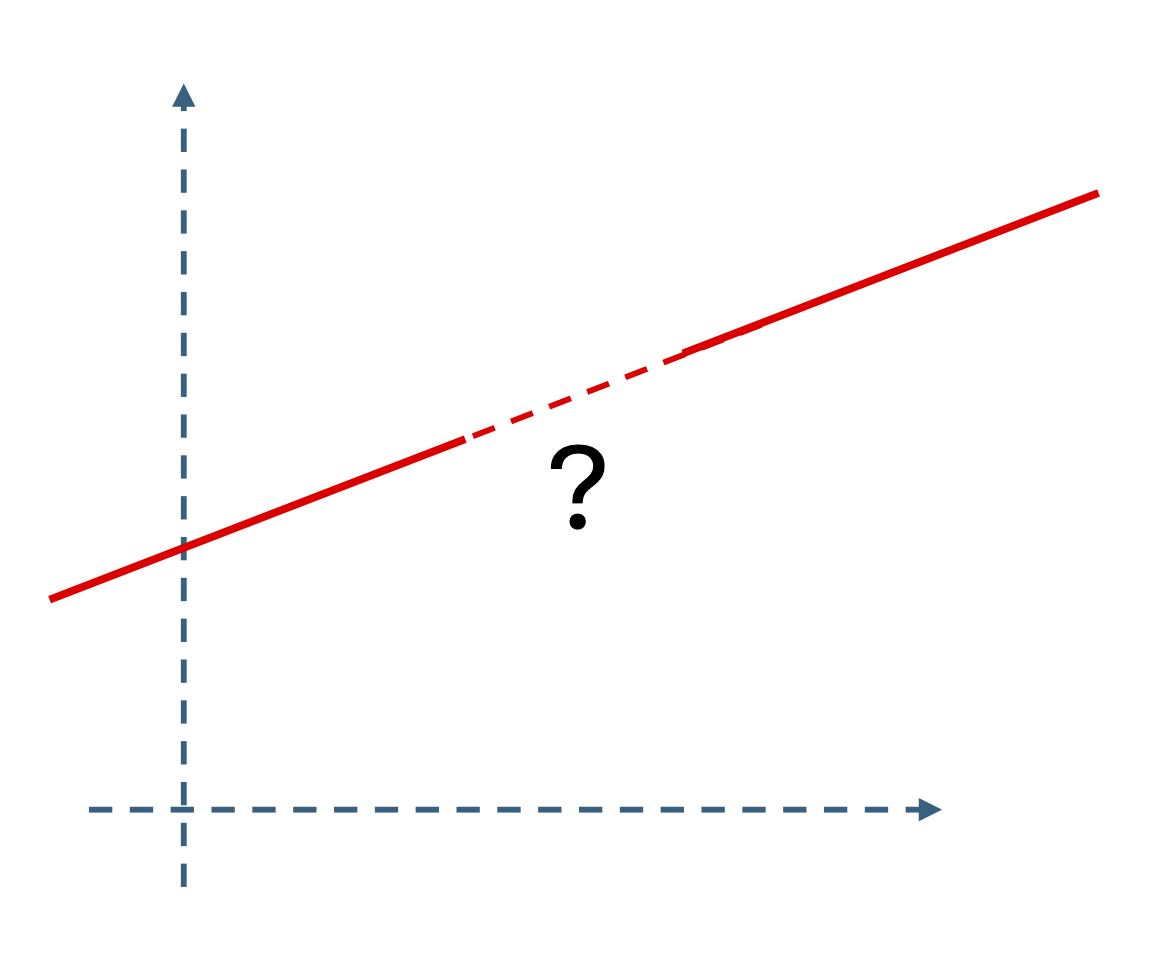
\includegraphics[height=0.28\linewidth]{\toplevelprefix/chapters/chapter1/figs/Completion-low-dim.png}     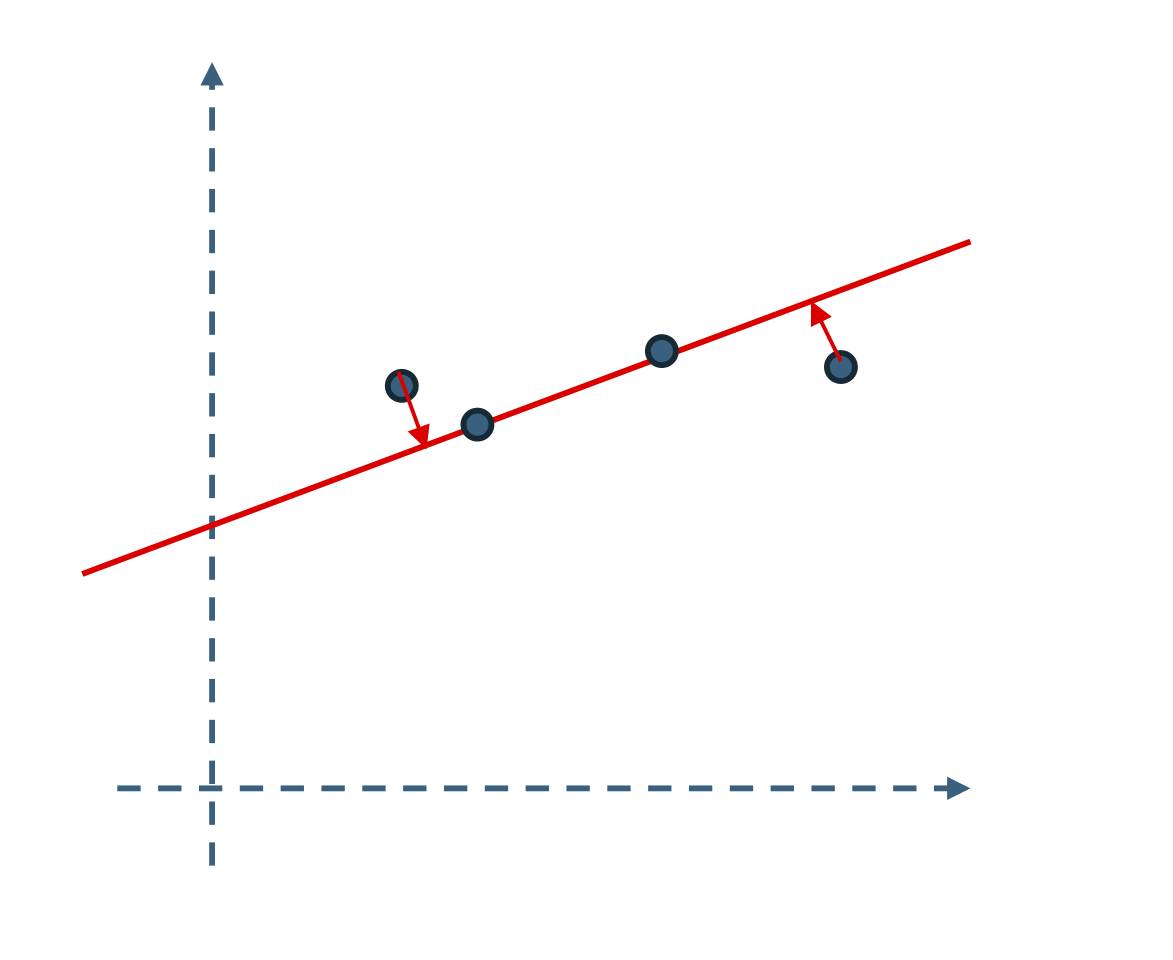
\includegraphics[height=0.28\linewidth]{\toplevelprefix/chapters/chapter1/figs/Denoising-low-dim.png} 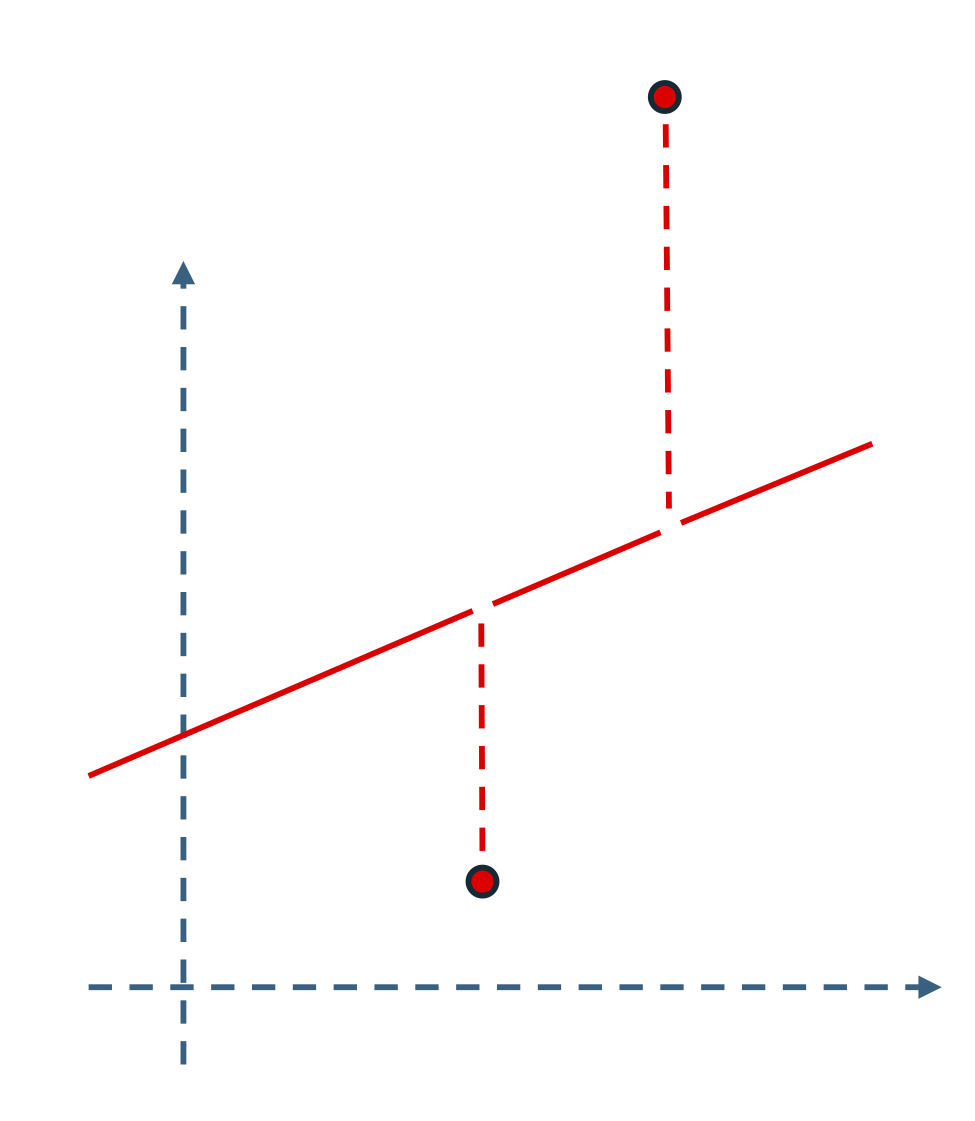
\includegraphics[height=0.32\linewidth]{\toplevelprefix/chapters/chapter1/figs/Correction-low-dim.png}
    \caption{Ilustrarea proprietăților unei structuri (liniare) cu dimensiuni reduse: permite completarea (stânga), îndepărtarea zgomotului (mijloc) și corectarea erorilor (dreapta).}
    \label{fig:low-dim-properties}
\end{figure}

De fapt, în condiții blânde, proprietățile de mai sus sunt generalizabile la multe alte structuri cu dimensiuni reduse în spații cu dimensiuni mari \cite{Wright-Ma-2022}. Interesant, după cum vom vedea în această carte, aceste proprietăți utile precum completarea și îndepărtarea zgomotului vor inspira metode eficiente pentru a învăța astfel de structuri cu dimensiuni reduse.

În cele de mai sus, pentru simplitate, am folosit doar cazul determinist pentru a introduce noțiunea importantă de predictibilitate și dimensionalitate redusă. Prin urmare, datele (sau segmentele eșantionate) se află precis pe anumite structuri geometrice precum subspații sau suprafețe. În practică, după cum am aluzionat înainte, există întotdeauna un anumit nivel de incertitudine sau aleatorie în date. În acest caz, putem presupune că datele au o distribuție de probabilitate, cu o funcție de densitate de probabilitate $p(\vx)$. Spunem că o distribuție este „cu dimensiuni reduse" dacă densitatea sa se concentrează în jurul unei structuri geometrice care este destul de cu dimensiuni reduse, să zicem un subspațiu, o suprafață sau un amestec al acestora, așa cum se arată în \Cref{fig:mixture-models}. Observați că, din punct de vedere practic, o astfel de funcție de densitate $p(\x)$, odată învățată, poate servi ca o prioritate foarte puternică pentru estimarea $\x$ pe baza observației parțiale, zgomotoase sau corupte, să zicem:
\begin{equation}
\y = f(\x) + \boldsymbol{n},
\end{equation}
prin calcularea estimării condiționate $\hat{\x}(\y) = \mathbb{E}(\x \mid \y)$ sau prin eșantionarea distribuției condiționate $\hat{\x}(\y) \sim p(\x\mid \y)$.\footnote{Tehnologiile moderne de AI generativă, cum ar fi generarea de imagini (condiționată), se bazează foarte mult pe acest fapt, așa cum vom elabora în \Cref{ch:conditional-inference}.}

Discuțiile noastre de mai sus au condus la principala și singura presupunere pe care această carte o va face pentru o abordare deductivă pentru a înțelege inteligența și rețelele profunde în special:
\begin{quote}
\textbf{Presupunerea Principală:} {\em Orice sisteme inteligente sau metode de învățare ar trebui și ar putea să se bazeze pe faptul că lumea este previzibilă, prin urmare distribuția eșantioanelor de date observate cu dimensiuni mari au suporturi cu dimensiuni reduse.}
\end{quote}
Întrebarea rămasă este cum să învățăm astfel de structuri cu dimensiuni reduse corect din datele cu dimensiuni mari, prin mijloace calculabile eficiente și eficace. După cum vom vedea în această carte, modelele parametrice care au fost bine studiate în abordările analitice clasice și modelele non-parametrice precum rețelele profunde care sunt populare în practica modernă sunt doar mijloace diferite pentru a atinge același obiectiv.

\section{Cum să Învățăm?}


\subsection{Abordări Analitice}
\label{sec:analytical}
Notați că, chiar dacă o funcție predictivă este tractabilă de calculat, nu implică faptul că este tractabilă sau scalabilă să învățăm această funcție dintr-un număr de segmente eșantionate. Desigur, o abordare clasică pentru a asigura că problemele sunt tractabile sau susceptibile la soluții eficiente este să facem presupuneri explicite despre familia de structuri cu dimensiuni reduse cu care avem de-a face. Istoric, din cauza calculului și datelor limitate, modelele analitice simple și idealiste au fost întotdeauna primele studiate deoarece oferă adesea soluții eficiente în formă închisă sau numerice. În plus, ele pot oferi perspective asupra problemelor mai generale și oferă adesea deja soluții utile pentru cazuri importante, deși limitate. În vremurile vechi, când resursele computaționale erau rare, modelele analitice care permiteau soluții eficiente în formă închisă sau numerice erau singurele cazuri care puteau fi implementate. {\em Structurile liniare} au devenit primele clase de modele care au fost studiate temeinic.

De exemplu, probabil cel mai simplu caz este să presupunem că datele sunt distribuite în jurul unui singur subspațiu cu dimensiuni reduse într-un spațiu cu dimensiuni mari. Sau într-un mod oarecum echivalent, se poate presupune că datele sunt distribuite conform unei gaussiene aproape degenerate cu dimensiuni reduse. Identificarea unui astfel de subspațiu sau gaussiană dintr-un număr finit de eșantioane (zgomotoase) este apoi problema clasică de analiză a componentelor principale (PCA) și au fost dezvoltați algoritmi eficienți pentru această clasă de modele \cite{JolliffeI2002}. Se poate face familia de modele din ce în ce mai complexă și expresivă. De exemplu, se poate presupune că datele sunt distribuite în jurul unui anumit amestec de componente cu dimensiuni reduse (subspații sau gaussiene cu dimensiuni reduse), ca în cazul analizei componentelor independente (ICA) \cite{Ans-1985}, învățării dicționarului (DL), analizei componentelor principale generalizate (GPCA) \cite{Vidal-GPCA}, sau clasa și mai generală de modele rare cu dimensiuni reduse care au fost studiate extensiv în ultimii ani în domenii precum detectarea comprimată \cite{Wright-Ma-2022}.

În jurul tuturor acestor familii de modele analitice, problema centrală de studiu este întotdeauna cum să identificăm {\em cel mai compact} model din cadrul fiecărei familii care se potrivește cel mai bine datelor date. Mai jos, oferim o relatare foarte scurtă a acestor modele analitice clasice, dar lăsăm un studiu mai sistematic pentru \Cref{ch:classic}. În teorie, aceste modele analitice ne-au oferit perspective extraordinare asupra proprietăților geometrice și statistice ale structurilor cu dimensiuni reduse. Ele oferă adesea soluții în formă închisă sau algoritmi eficienți și scalabili care sunt foarte utili pentru date ale căror distribuții pot fi bine aproximate de astfel de modele. Mai important, pentru probleme mai generale, ele ne oferă o înțelegere generală despre cât de ușoară sau dificilă poate fi problema identificării structurilor cu dimensiuni reduse și care sunt ideile de bază pentru a aborda o astfel de problemă.




\subsubsection{Sisteme Dinamice Liniare}
\label{sec:linear-systems}

\paragraph{Filtrul Wiener.}

După cum am discutat înainte în \Cref{sec:predictability}, o sarcină principală a inteligenței este să învețe ceea ce este previzibil în secvențele de observații. Probabil cea mai simplă clasă de secvențe previzibile, sau semnale, sunt generate printr-un proces {\em liniar invariant în timp} (LTI):
\begin{equation}
    x[n] = h[n]*z[n] + \epsilon[n],
    \label{eqn:Wiener-model}
\end{equation}
unde $z$ este intrarea și $h$ este funcția de răspuns la impuls.\footnote{În mod normal, se presupune că $h$ are anumite structuri frumoase, să zicem lungime finită sau spectru limitat.} Aici $\epsilon[n]$ este un anumit zgomot aditiv în observații. Problema este că, date fiind procesul de intrare $\{z[n]\}$ și observațiile procesului de ieșire $\{x[n]\}$, cum să găsim $h[n]$ optim astfel încât $\hat x[n] = h[n]*z[n]$ să prezică $x[n]$ într-un mod optim. În general, măsurăm calitatea predicției prin eroarea medie pătrată minimă (MMSE):
\begin{equation}
    \min_{h} \mathbb{E} \big[\epsilon[n]^2\big] = \mathbb{E} \big[\|x[n] - h[n]*z[n]\|_2^2\big].
\end{equation}
Soluția optimă $h[n]$ este denumită un filtru (de îndepărtare a zgomotului). Norbert Wiener, aceeași persoană care a inițiat mișcarea Cibernetică, a studiat această problemă în anii 1940 și a dat o soluție elegantă în formă închisă cunoscută sub numele de {\em filtrul Wiener} \cite{Wiener-1942,Wiener-1949}. Aceasta a devenit unul dintre cele mai fundamentale rezultate în domeniul Procesării Semnalelor.

\paragraph{Filtrul Kalman.}
Ideea de îndepărtare a zgomotului sau filtrare pentru un proces dinamic a fost extinsă mai târziu la un sistem liniar invariant în timp descris de un model de spațiu de stare (finit-dimensional) de Rudolph Kalman în anii 1960:
\begin{equation}
    \z[n] = \boldsymbol{A} \z[n-1] + \boldsymbol{B}\boldsymbol{u}[n] + \boldsymbol{\epsilon}[n].
    \label{eqn:linear-state-space}
\end{equation}
Problema este cum putem estima starea sistemului $\z[n]$ din observații zgomotoase de forma: \begin{equation}\x[n] = \boldsymbol{C} \z[n] + \boldsymbol{w}[n],
\label{eqn:Kalman-model}
\end{equation}
unde $\boldsymbol{w}$ este un anumit zgomot (alb). Estimatorul de stare cauzal optim\footnote{Ceea ce înseamnă că estimarea poate folosi doar observații până la pasul de timp curent $n$. Filtrul Kalman este întotdeauna cauzal, în timp ce filtrul Wiener nu trebuie să fie.} care minimizează eroarea de predicție de tip MMSE
\begin{equation}
    \min \mathbb{E}\big[ \|\x[n] - \boldsymbol{C}\z[n]\|_2^2\big]
\end{equation}
este dat în formă închisă de așa-numitul {\em filtru Kalman} \cite{kalman1960new}. Acesta este unul dintre pilonii Teoriei Moderne a Controlului deoarece ne permite să estimăm starea unui sistem dinamic din observațiile sale zgomotoase. Apoi se poate introduce ulterior un feedback de stare (liniar), să zicem de forma $\boldsymbol{u}[n] = \boldsymbol{F} \hat{\boldsymbol{z}}[n]$, și să facem sistemul în buclă închisă complet autonom, așa cum am văzut în ecuația \eqref{eqn:recursive-closed-loop}.

\paragraph{Identificarea Sistemelor Dinamice Liniare.}
Pentru a deriva filtrul Kalman, parametrii sistemului $(\boldsymbol{A}, \boldsymbol{B}, \boldsymbol{C})$ sunt presupuși a fi cunoscuți. Dacă nu sunt dați în avans, ar fi o problemă mai dificilă cunoscută sub numele de {\em identificarea sistemului}: cum să {\em învățăm} parametrii $(\boldsymbol{A}, \boldsymbol{B}, \boldsymbol{C})$ din (multe eșantioane ale) secvenței de intrare $\{\boldsymbol{u}[n]\}$ și secvenței de observație $\{\x[n]\}$. Aceasta este o problemă clasică în teoria sistemelor. Dacă sistemul este liniar, se poate arăta că secvențele de intrare și ieșire $\{\boldsymbol{u}[n], \x[n]\}$ s-ar afla împreună pe un anumit subspațiu cu dimensiuni reduse\footnote{care are aceeași dimensiune ca ordinea modelului de spațiu de stare \eqref{eqn:linear-state-space}.}. Prin urmare, problema de identificare este în esență echivalentă cu identificarea acestui subspațiu cu dimensiuni reduse \cite{OverscheeP1996,Liu-2009-CDC,Liu-2010-SIAM}.

Notați că problemele de mai sus au două lucruri în comun: în primul rând, secvențele sau semnalele (fără zgomot) sunt presupuse a fi generate de o familie explicită de modele parametrice; în al doilea rând, aceste modele sunt în esență toate liniare. Deci, conceptual, fie $\x_o$ o variabilă aleatorie a cărei distribuție „adevărată" este susținută pe un subspațiu liniar cu dimensiuni reduse, să zicem $S$. Într-o mare măsură, filtrul Wiener și filtrul Kalman încearcă toate să estimeze un astfel de $\x_o$ din observațiile sale zgomotoase:
\begin{equation}
    \x = \x_o + \boldsymbol{\epsilon}, \quad \x_o \sim S,
\end{equation}
unde $\boldsymbol{\epsilon}$ este de obicei un zgomot gaussian aleatoriu (sau proces). Prin urmare, în esență, soluțiile lor se bazează toate pe identificarea unui subspațiu liniar cu dimensiuni reduse care se potrivește cel mai bine datelor observate (zgomotoase). Apoi, proiectând datele pe acest subspațiu, se obțin operațiile optime de îndepărtare a zgomotului, toate în formă închisă.


\subsubsection{Modele Liniare și Mixte Liniare}
\label{sec:PCA-ICA}
\paragraph{Analiza Componentelor Principale.}
Din problemele de mai sus în procesarea clasică a semnalelor și identificarea sistemelor, vedem că sarcina principală din spatele tuturor acestor probleme este să învățăm din observații zgomotoase un {\em singur} subspațiu liniar cu dimensiuni reduse. Matematic, putem modela o astfel de structură ca:
\begin{equation}
    \x = \boldsymbol{u}_1 z_1 + \boldsymbol{u}_2 z_2 + \cdots + \boldsymbol{u}_d z_d + \boldsymbol{\epsilon} =  \boldsymbol{U} \z + \boldsymbol{\epsilon}, \quad \boldsymbol{U} \in \mathbb{R}^{D\times d}
    \label{eqn:PCA-model}
\end{equation}
unde $\boldsymbol{\epsilon} \in \mathbb{R}^D$ este un anumit zgomot aleatoriu mic. \Cref{fig:PCA} ilustrează o astfel de distribuție cu două componente principale.
\begin{figure}
    \centering
    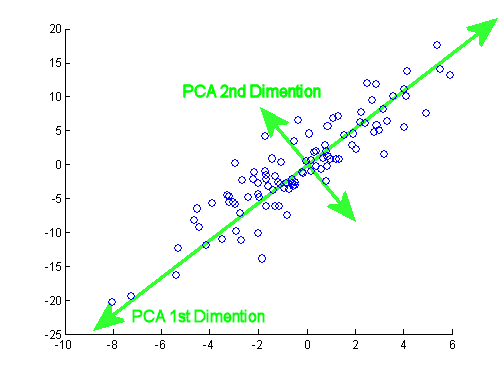
\includegraphics[width=0.5\linewidth]{\toplevelprefix/chapters/chapter1/figs/PCA.png}
    \caption{O distribuție cu două componente principale.}
    \label{fig:PCA}
\end{figure}
Problema este să găsim baza subspațiului $\boldsymbol{U}$ din multe eșantioane de $\x$. O abordare tipică pentru a estima subspațiul $\boldsymbol{U}$ este să minimizăm varianța zgomotului, cunoscută și sub numele de eroarea medie pătrată minimă (MMSE):
\begin{equation}
    \min_{\boldsymbol{U}} \mathbb{E}\big[\|\boldsymbol{\epsilon}\|_2^2\big] = \mathbb{E}\big[\|\x - \boldsymbol{U} \z\|_2^2\big].
\end{equation}
Observați că aceasta este în esență o sarcină de îndepărtare a zgomotului: odată ce baza $\boldsymbol{U}$ este găsită corect, putem îndepărta zgomotul din eșantionul zgomotos $\x$ proiectându-l pe subspațiul cu dimensiuni reduse extins de $\boldsymbol{U}$ ca
\begin{equation}
\x \rightarrow \hat \x = \boldsymbol{U}\boldsymbol{U}^\top \x.
\end{equation}
Dacă zgomotul este mic și dacă am învățat subspațiul corect cu dimensiuni reduse $\boldsymbol{U}$, ar trebui să ne așteptăm $\x \approx \hat \x$. Adică, PCA este un caz special de auto-codare:
\begin{equation}
    \x   \xrightarrow{\hspace{2mm} \boldsymbol{U}^\top\hspace{2mm}} \z  \xrightarrow{\hspace{2mm} \boldsymbol{U} \hspace{2mm}} \hat \x.
       \label{eqn:auto-encoding-PCA}
\end{equation}
Doar că aici, din cauza structurii simple a datelor, codificatorul $\mathcal{E}$ și decodificatorul $\mathcal{D}$ devin ambii operatori liniari simpli (proiectare și ridicare).

Aceasta este o problemă clasică în statistică cunoscută sub numele de Analiza Componentelor Principale (PCA). A fost studiată pentru prima dată de Pearson în 1901 \cite{Pearson1901} și mai târziu independent de Hotelling în 1933 \cite{Hotelling1933}. Acest subiect este rezumat sistematic în cartea clasică \cite{Jolliffe1986,JolliffeI2002}.
În plus, se poate presupune explicit că datele $\x$ sunt distribuite conform unei singure gaussiene cu dimensiuni reduse:
\begin{equation}
    \x \sim \mathcal{N}(\boldsymbol{0}, \boldsymbol{U}\boldsymbol{U}^\top + \sigma \I), \quad \boldsymbol{U} \in \mathbb{R}^{D\times d},
\end{equation}
care este echivalent cu presupunerea că $\z$ în modelul PCA de mai sus \eqref{eqn:PCA-model} este o distribuție normală standard.
Aceasta este cunoscută ca PCA Probabilistică \cite{TippingM1999}.

În această carte, vom revizita PCA în \Cref{ch:classic}, din perspectiva învățării unei distribuții cu dimensiuni reduse. Obiectivul nostru este să folosim acest model simplu și idealist pentru a transmite unele dintre ideile cele mai fundamentale pentru învățarea unei reprezentări compacte pentru o distribuție cu dimensiuni reduse, inclusiv noțiunea importantă de compresie prin îndepărtarea zgomotului și autocodare pentru o reprezentare consistentă.

\paragraph{Analiza Componentelor Independente.}
Analiza componentelor independente (ICA) a fost propusă inițial de \cite{Ans-1985} ca un model clasic pentru {\em învățarea unei reprezentări bune}. De fapt, a fost propusă inițial ca un model matematic simplu pentru memoria noastră. Modelul ICA ia o formă înșelător de similară cu modelul PCA de mai sus \eqref{eqn:PCA-model} presupunând că variabila aleatorie observată $\x$ este o suprapunere liniară a mai multor componente independente $z_i$:
\begin{equation}
    \x = \boldsymbol{u}_1 z_1 + \boldsymbol{u}_2 z_2 + \cdots + \boldsymbol{u}_d z_d  + \boldsymbol{\epsilon} =  \boldsymbol{U} \z + \boldsymbol{\epsilon}.
    \label{eqn:ICA-model}
\end{equation}
Cu toate acestea, aici componentele $z_i$ sunt presupuse a fi variabile {\em non-gaussiene} independente. De exemplu, o alegere populară este
\begin{equation}
    z_i = \sigma_i \cdot w_i, \quad \sigma_i \sim B(1,p),
    \label{eqn:ICA-modes}
\end{equation}
unde $\sigma_i$ este o variabilă Bernoulli și $w_i$ ar putea fi o valoare constantă sau o altă variabilă aleatorie, să zicem gaussiană.\footnote{Chiar dacă $w$ este gaussiană, $\sigma w$ nu mai este o variabilă gaussiană!} Problema ICA încearcă să identifice atât $\boldsymbol{U}$ cât și $\z$ din eșantioane observate de $\x$. \Cref{fig:ICA-PCA} ilustrează diferența dintre ICA și PCA.

\begin{figure}
    \centering
    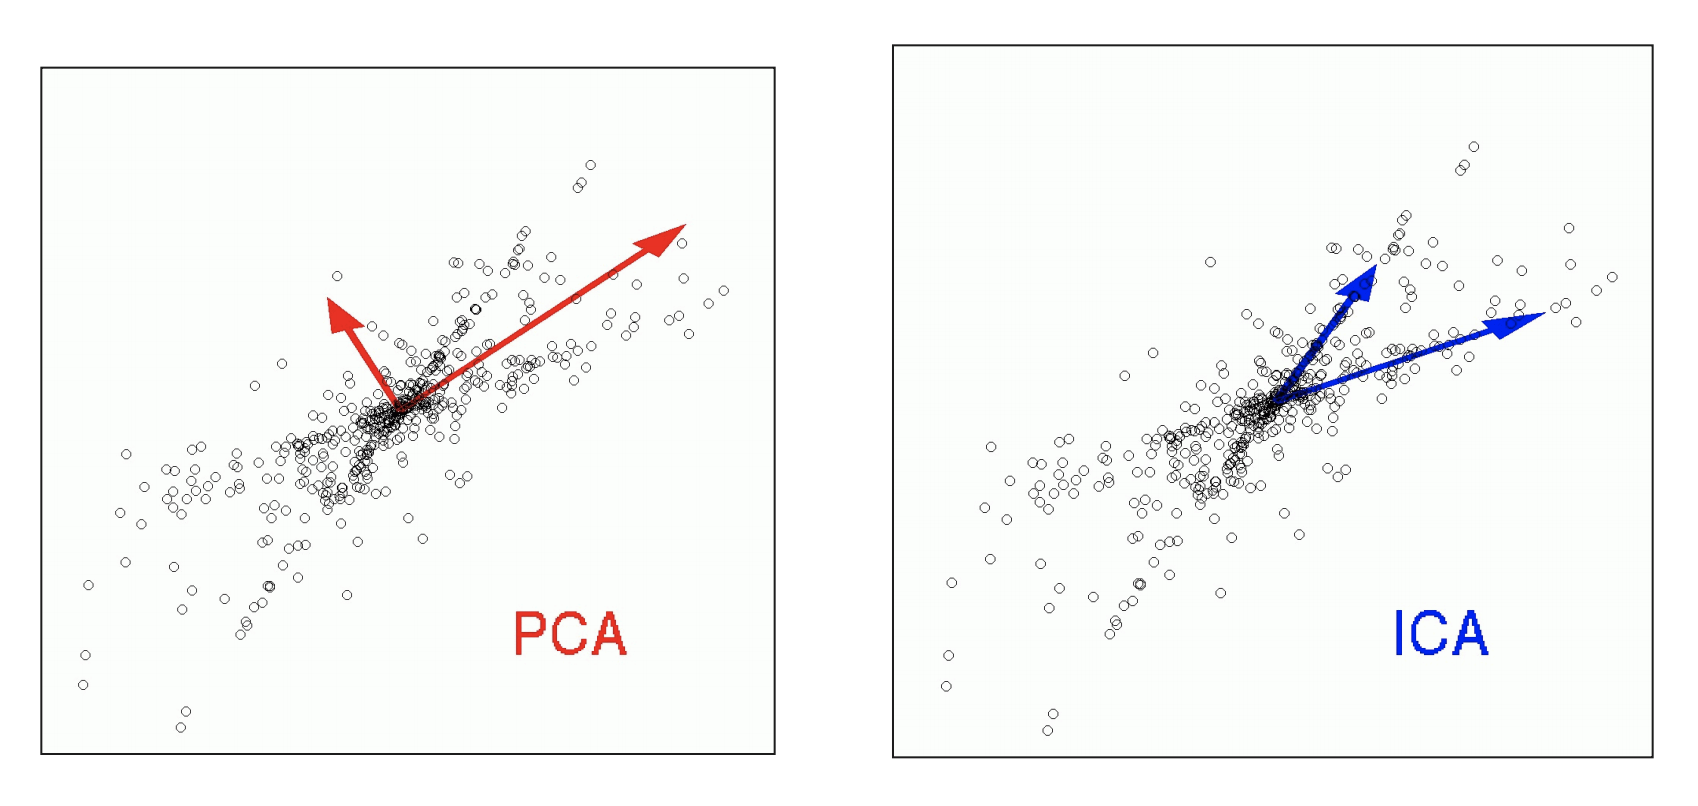
\includegraphics[width=0.7\linewidth]{\toplevelprefix/chapters/chapter1/figs/PCA_ICA.png}
    \caption{PCA (stânga) versus ICA (dreapta).}
    \label{fig:ICA-PCA}
\end{figure}

Deși maparea (de decodare) de la $\z$ la $\x$ pare liniară și ușoară odată ce $\boldsymbol{U}$ și $\z$ sunt învățate, maparea (de codare) de la $\x$ la $\z$ poate fi complicată și s-ar putea să nu fie reprezentată de o simplă mapare liniară. Prin urmare, ICA oferă în general o autocodare de forma:
\begin{equation}
    \x   \xrightarrow{\hspace{2mm} \mathcal{E}\hspace{2mm}} \z  \xrightarrow{\hspace{2mm} \boldsymbol{U} \hspace{2mm}} \hat \x.
       \label{eqn:auto-encoding-ICA}
\end{equation}
Prin urmare, spre deosebire de PCA, ICA este puțin mai dificil de analizat și rezolvat. În anii 1990, cercetători precum Erkki Oja și Aapo Hyv\"{a}rinen \cite{hyvarinen-1997,Hyvrinen-2000} au adus contribuții teoretice și algoritmice semnificative la ICA. În \Cref{ch:classic}, vom studia și vom oferi o soluție la ICA din care maparea de codare $\mathcal{E}$ va deveni clară.



\paragraph{Structuri Rare și Detectare Comprimată.}
După cum se poate vedea, dacă $p$ în \eqref{eqn:ICA-modes} este foarte mic, probabilitatea ca oricare dintre componente să fie diferită de zero este mică. În acest caz, spunem că $\x$ este generat rar și se concentrează pe un set de subspații liniare de dimensiune $k = p \cdot d$. Prin urmare, într-o oarecare măsură, putem extinde modelul ICA de mai sus la o familie mai generală de structuri cu dimensiuni reduse cunoscută sub numele de modele rare.

Un model $k$-rar este definit ca fiind format din setul tuturor {\em vectorilor $k$-rari}:
\begin{equation}
    \mathcal{Z} = \{\z \in \mathbb{R}^n \mid \|\z\|_0 \le k\},
\end{equation}
unde $\| \cdot \|_0$ este norma $\ell^0$ care numără numărul de intrări diferite de zero într-un vector $\z$. Adică, $\mathcal{Z}$ este reuniunea tuturor subspațiilor $k$-dimensionale care se aliniază cu axele de coordonate, așa cum este ilustrat în \Cref{fig:mixture-models} stânga. O problemă importantă în procesarea clasică a semnalelor și statistică este cum să recuperăm un vector rar $\z$ din observațiile sale liniare:
\begin{equation}
    \x = \boldsymbol{A} \z + \boldsymbol{\epsilon}, \quad \boldsymbol{A} \in \mathbb{R}^{m\times n}
    \label{eqn:sparse-model}
\end{equation}
unde $\boldsymbol{A}$ este dat, dar de obicei $m < n$ și $\boldsymbol{\epsilon}$ este un anumit zgomot mic. Această problemă aparent benignă se dovedește a fi NP-grea de calculat și este chiar greu de aproximat (vezi cartea \cite{Wright-Ma-2022} pentru detalii).

Deci, în ciuda unei istorii foarte bogate și lungi de studiu care poate fi datată încă din secolul al XVIII-lea \cite{Boscovichca1750}, nu a existat niciun algoritm dovedit eficient pentru a rezolva această clasă de probleme, deși au fost propuși și dezvoltați mulți algoritmi euristici între anii 1960 și 1990. Unii sunt destul de eficienți în practică, dar fără nicio justificare riguroasă. O descoperire majoră a venit la începutul anilor 2000 când câțiva matematicieni renumiți, inclusiv David Donoho, Emmanuel Cand\`{e}s și Terence Tao \cite{donoho2005neighborly,Candes2005,CandesE2005-IT} au stabilit un cadru teoretic riguros care ne permite să caracterizăm condiții precise în care problema de recuperare rară poate fi rezolvată eficient și eficace, să zicem printr-o minimizare convexă $\ell^1$:
\begin{equation}
    \min \|\z\|_1 \quad \mbox{subiect la} \quad \| \x - \boldsymbol{A}\z\|_2 \le \epsilon,
\end{equation}
unde $\|\cdot \|_1$ este norma $\ell^1$ care promovează raritatea unui vector și $\epsilon$ este o constantă mică. Orice soluție la această problemă oferă în esență o mapare de codare rară:
\begin{equation}
    \x   \xrightarrow{\hspace{2mm} \mathcal{E} \hspace{2mm}}  \z.
       \label{eqn:decoding-sparse}
\end{equation}
Vom oferi o scurtă relatare a unui astfel de algoritm, prin urmare mapare, în \Cref{ch:classic} care va dezvălui conexiuni fundamentale interesante între codarea rară și învățarea profundă.\footnote{Deși similaritățile dintre algoritmii pentru codarea rară și rețelele profunde au fost observate încă din 2010 \cite{gregor2010learning}.}

După cum se dovedește, condițiile în care minimizarea $\ell^1$ reușește sunt surprinzător de generale. Numărul minim de măsurători $m$ necesar pentru o recuperare de succes este doar proporțional cu dimensiunea intrinsecă a datelor $k$. Aceasta este acum cunoscută sub numele de fenomenul {\em detectării comprimate} \cite{CandesE2006-ICM}. Mai mult, acest fenomen nu este unic pentru structurile rare. Se aplică și la familii foarte largi de structuri cu dimensiuni reduse, cum ar fi matricile de rang mic etc. Aceste rezultate au schimbat fundamental înțelegerea noastră despre recuperarea structurilor cu dimensiuni reduse în spații cu dimensiuni mari. Această inversare dramatică a norocului cu analiza datelor cu dimensiuni mari a fost chiar sărbătorită ca {\em „binecuvântarea dimensionalității"} de David Donoho \cite{DonohoD2000}, spre deosebire de credința pesimistă tipică în „blestemul dimensionalității" pentru problemele cu dimensiuni mari. Acest corp coerent și complet de rezultate a fost organizat sistematic în cartea \cite{Wright-Ma-2022}.

Din perspectivă computațională, nu se poate supraestima semnificația acestui nou cadru. A schimbat fundamental viziunile noastre despre o clasă importantă de probleme despre care se credea anterior că sunt în mare parte intractabile. Ne-a permis să dezvoltăm algoritmi extrem de eficienți care se scalează grațios cu dimensiunea problemei, făcând astfel problema recuperării rare de la:
\begin{equation}
    \mbox{\textbf{intractabilă}} \;
   \Longrightarrow \; \mbox{\textbf{tractabilă}} \; \Longrightarrow \;
   \mbox{\textbf{scalabilă}}.
\end{equation}
Acești algoritmi vin și cu garanții teoretice riguroase ale corectitudinii lor, date cerințe precise în date și calcul. Natura riguroasă și precisă a acestei abordări este aproape opusă celei a practicării rețelelor neuronale profunde, care este în mare parte empirică. Cu toate acestea, în ciuda stilurilor și standardelor lor aparent opuse, știm acum că ambele abordări împărtășesc un obiectiv comun: {\em încercarea de a urmări structuri cu dimensiuni reduse în spații cu dimensiuni mari.}

\paragraph{Învățarea Dicționarului.}
Conceptual, o problemă și mai dificilă decât problema codării rare \eqref{eqn:sparse-model} este atunci când matricea de observație $\boldsymbol{A}$ nu este nici măcar cunoscută în avans și trebuie să învățăm $\boldsymbol{A}$ dintr-un set de observații (posibil zgomotoase), să zicem $\X = [\x_1, \x_2, \ldots, \x_n]$:
\begin{equation}
    \X = \boldsymbol{A} \Z + \boldsymbol{E}, \quad \boldsymbol{A} \in \mathbb{R}^{m\times n}.
    \label{eqn:dictionary-learning}
\end{equation}
Aici ni se dă doar $\X$ dar nu și $\Z = [\z_1, \z_2, \ldots, \z_n]$ corespunzător sau termenul de zgomot $\boldsymbol{E}= [\boldsymbol{\epsilon}_1, \boldsymbol{\epsilon}_2, \ldots, \boldsymbol{\epsilon}_n]$, cu excepția faptului că știm că $\z_i$ sunt rari. Aceasta este cunoscută sub numele de problema {\em învățării dicționarului}, care poate fi văzută ca o generalizare a problemei ICA \eqref{eqn:ICA-model} discutată mai devreme. Cu alte cuvinte, dată fiind distribuția datelor $\X$ ca fiind imaginea unei distribuții rare standard $\Z$ sub o transformare liniară $\boldsymbol{A}$, am dori să învățăm $\boldsymbol{A}$ și maparea sa „inversă" $\mathcal{E}$ astfel încât să obținem un autocodor:
\begin{equation}
    \X   \xrightarrow{\hspace{2mm} \mathcal{E} \hspace{2mm}}  \Z \xrightarrow{\hspace{2mm} \boldsymbol{A} \hspace{2mm}} \X?
       \label{eqn:decoding-DL}
\end{equation}

Se poate vedea ce au în comun PCA, ICA și Învățarea Dicționarului este că toate presupun că distribuția datelor este susținută în jurul structurilor liniare sau mixte liniare cu dimensiuni reduse. Toate necesită învățarea unei baze (globale sau locale) a structurilor liniare, din eșantioane probabil zgomotoase ale distribuției. În \Cref{ch:classic}, vom studia cum să identificăm structuri cu dimensiuni reduse prin aceste modele clasice. În special, vom vedea un fapt interesant și important: toate aceste modele (pe bucăți) liniare cu dimensiuni reduse pot fi învățate eficient și eficace de același tip de algoritmi rapizi, cunoscuți sub numele de {\em iterație de putere} \cite{Zhai-2020}. Deși modelele liniare sau mixte liniare de mai sus sunt oarecum prea simpliste sau idealiste pentru majoritatea datelor din lumea reală, înțelegerea acestor modele este un prim pas important către înțelegerea distribuțiilor mai generale cu dimensiuni reduse.

\subsubsection{Distribuții Generale}\label{sec:denoising-intro}

Distribuțiile datelor din lumea reală, cum ar fi imaginile, videoclipurile și sunetul, sunt prea complexe pentru a fi modelate de modelele liniare oarecum idealiste de mai sus. În mod normal, nu știm {\em a priori} din care familie de modele parametrice sunt generate.\footnote{Deși în istorie au existat multe încercări de a dezvolta modele analitice pentru aceste date, cum ar fi câmpuri aleatorii sau procese stochastice pentru date imagistice \cite{Mumford-1999}, așa cum am discutat în secțiunea anterioară.} În practică, de obicei avem doar multe eșantioane din distribuțiile lor -- distribuțiile empirice. Evident, în astfel de cazuri, în mod normal nu ne putem aștepta să avem soluții în formă închisă pentru structurile lor cu dimensiuni reduse, nici pentru operatorii de îndepărtare a zgomotului rezultați.\footnote{Spre deosebire de cazurile PCA, filtrul Wiener și filtrul Kalman.} Deci trebuie să dezvoltăm o soluție mai generală pentru aceste distribuții empirice, nu neapărat în formă închisă, dar cel puțin calculabilă eficient. Dacă am face acest lucru corect, soluțiile la modelele liniare menționate anterior ar trebui să devină cazurile lor speciale.

\paragraph{Îndepărtarea zgomotului.} În anii 1950, statisticienii au devenit interesați de problema îndepărtării zgomotului din date extrase dintr-o distribuție arbitrară. Fie $\x_o$ o variabilă aleatorie cu funcția de densitate de probabilitate $p_o(\cdot)$. Deci, dacă observăm o versiune zgomotoasă a $\x_o$:
\begin{equation}
    \x = \x_o + \sigma \vg,
\end{equation}
unde $\vg \sim \dNorm(\vzero, \vI)$ este zgomot gaussian standard și $\sigma$ este nivelul de zgomot al observației. Fie $p(\cdot)$ funcția de densitate de probabilitate a $\x$,\footnote{Adică, $p(\x) = \int_{-\infty}^{\infty} \phi_{\sigma}(\x - \z)p_o(\z) \odif{\z}$, unde $\phi_{\sigma}$ este funcția de densitate a distribuției gaussiene $\mathcal{N}(\boldsymbol{0}, \sigma^2 \boldsymbol{I})$.} Uimitor, așteptarea posterioară a $\x_o$ dat $\x$ poate fi calculată printr-o formulă elegantă, cunoscută sub numele de formula lui Tweedie \cite{Robbins1956AnEB}:\footnote{Herbert Robbins a dat creditul pentru această formulă lui Maurice Kenneth Tweedie din corespondența lor personală.}
\begin{equation}
    \hat \x_o = \mathbb{E}[\x_o\mid \x] = \x + \sigma^2 \nabla \log p(\x).
\end{equation}
După cum se poate vedea din formulă, funcția $\nabla \log p(\x)$ joacă un rol foarte special în îndepărtarea zgomotului din observația $\x$ aici. Zgomotul $\vg$ poate fi estimat explicit ca
\begin{equation}
    \hat{\vg} = \frac{\x - \hat \x_o}{\sigma} = -\sigma \nabla \log p(\x),
\end{equation}
pentru care avem nevoie doar să cunoaștem distribuția $p(\cdot)$ a $\x$, nu adevărul de bază $p_o(\cdot)$ pentru $\x_o$. O implicație importantă a acestui rezultat este că, dacă adăugăm zgomot gaussian la orice distribuție, procesul de îndepărtare a zgomotului poate fi făcut ușor dacă putem cumva să obținem funcția $\nabla \log p(\x)$.

Deoarece acesta este un rezultat atât de important și util, a fost redescoperit și folosit în multe contexte și domenii diferite. De exemplu, după formula lui Tweedie \cite{Robbins1956AnEB}, a fost redescoperită câțiva ani mai târziu de \cite{Miyasawa61}. La începutul anilor 2000, funcția $\nabla \log p(\x)$ a fost redescoperită din nou în contextul învățării unei distribuții generale și a fost numită „funcția de scor" de Aapo Hyv\"{a}rinen \cite{hyvarinen05a}. Dar conexiunea sa cu îndepărtarea zgomotului (Bayesian empiric) a fost recunoscută curând de \cite{Vincent2011}.
Generalizări la alte distribuții de măsurare (dincolo de zgomotul gaussian) au fost făcute de grupul lui Eero Simoncelli \cite{Raphan10} și aplicate ulterior la îndepărtarea zgomotului din imagini \cite{Kadkhodaie21a,ho2020denoising}.

\begin{figure}
    \centering
    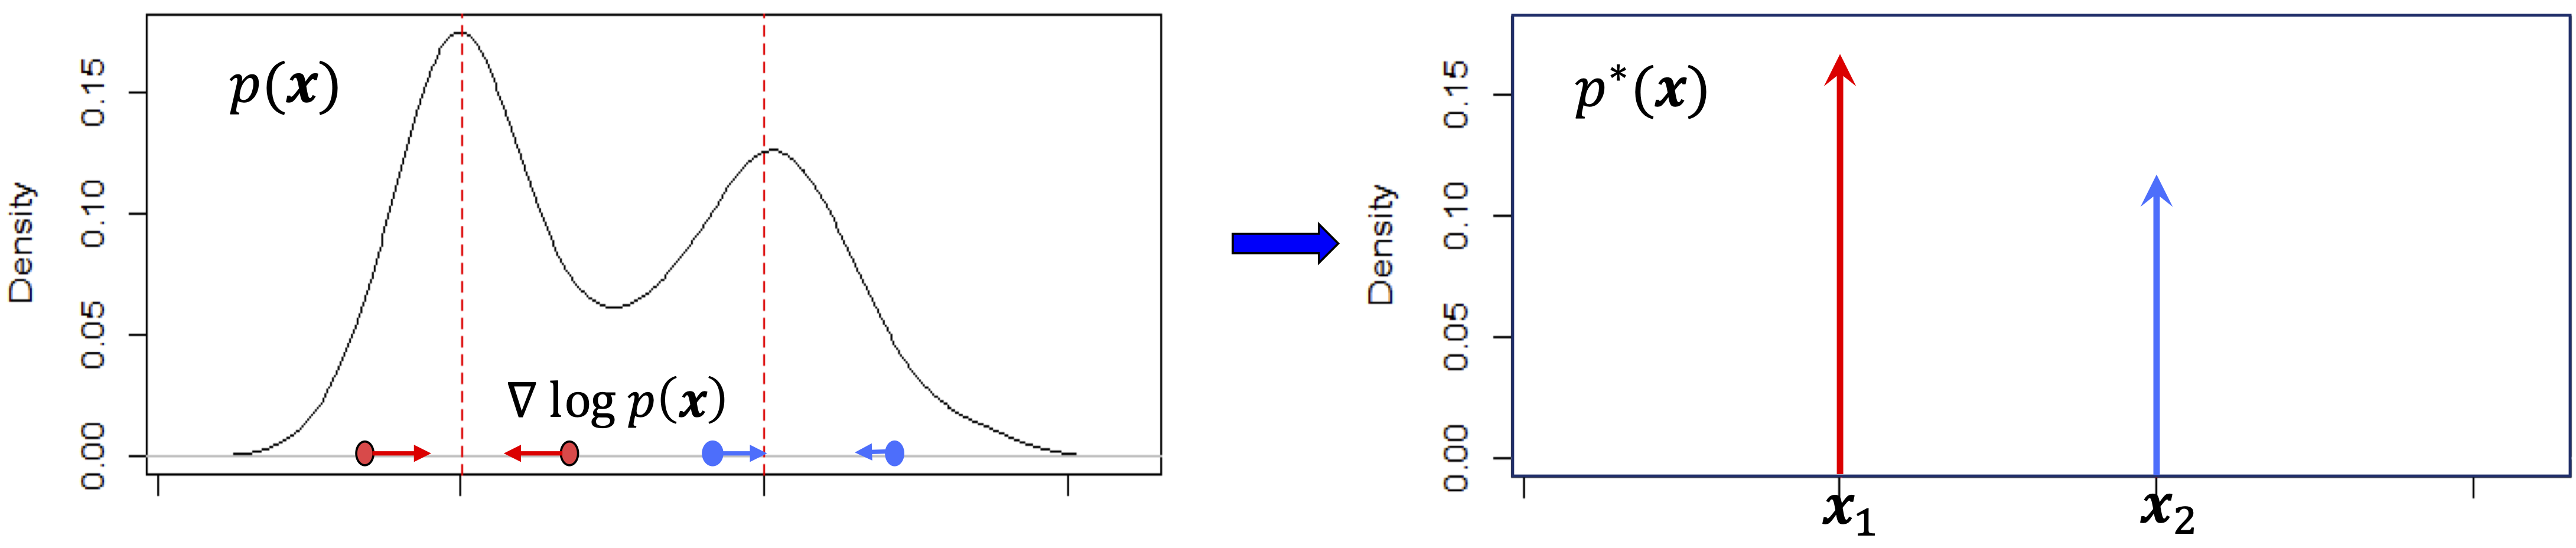
\includegraphics[width=1\linewidth]{\toplevelprefix/chapters/chapter1/figs/Density-compress.png}
    \caption{Interpretarea geometrică a unei funcții de scor $\nabla \log p(\x)$ pentru o distribuție cu densitatea $p(\x)$ pe stânga. Operația generată de funcția de scor împinge distribuția către zone cu densitate mai mare. Obiectivul este ca, printr-o anumită măsură de compactitate (de exemplu, entropie sau lungime de codare), distribuția rezultată să fie mai „comprimată". În cele din urmă, distribuția converge la una care are un suport cu dimensiuni mai reduse, așa cum $p^*(\x)$ arătat pe dreapta.}
    \label{fig:score-function}
\end{figure}

\paragraph{Minimizarea entropiei.} De fapt, această funcție are o interpretare foarte intuitivă din punct de vedere teoretic-informațional și geometric. Notați că în teoria informației $-\log p(\x)$ corespunde în general numărului de biți necesari pentru a codifica $\x$\footnote{cel puțin în cazul unei variabile discrete, așa cum vom explica mai detaliat în \Cref{ch:compression}.}. Gradientul $\nabla \log p(\x)$ indică o direcție în care densitatea este mai mare, așa cum se arată în \Cref{fig:score-function} stânga. Numărul de biți necesari pentru a codifica $\x$ scade dacă se mișcă în acea direcție. Prin urmare, efectul general al operatorului $\nabla \log p(\x)$ este să împingă distribuția să „se micșoreze" către zone cu densitate mai mare. De fapt, se poate arăta formal că entropia (diferențială) a distribuției
\begin{equation}
H(\x) = - \int p(\boldsymbol{w}) \log p(\boldsymbol{w}) \odif{\boldsymbol{w}}    \end{equation}
scade într-adevăr sub o astfel de operație (vezi \Cref{ch:compression} și \Cref{app:diffusion-denoising}). Prin urmare, dacă o codificăm cu o carte de coduri optimă, lungimea/rata generală de codare a distribuției rezultate este redusă, prin urmare mai „comprimată". Intuitiv, ne putem imagina că, dacă repetăm un astfel de proces de îndepărtare a zgomotului la nesfârșit, distribuția va ajunge în cele din urmă să se micșoreze la una a cărei masă este concentrată pe un suport de dimensiune inferioară. De exemplu, distribuția $p(\x)$ prezentată în stânga din \Cref{fig:score-function}, sub acțiunea funcției de scor $\nabla \log p(\x)$, va converge în cele din urmă la distribuția $p^*(\x)$ din dreapta\footnote{Strict vorbind, $p^*(\x)$ este o distribuție a cărei densitate este o funcție generalizată: $p^*(\x) = p^*(\x_1)\delta(\x-\x_1) + p^*(\x_2) \delta(\x-\x_2)$, cu $p^*(\x_1) + p^*(\x_2) = 1$.}:
\begin{equation}
H(\x) = - \int p(\boldsymbol{w}) \log p(\boldsymbol{w}) \odif{\boldsymbol{w}}  \quad \xrightarrow{\hspace{1mm} \mbox{descrescând} \hspace{1mm}} \quad H^*(\x) = - \int p^*(\boldsymbol{w}) \log p^*(\boldsymbol{w}) \odif{\boldsymbol{w}}.
\end{equation}
Strict vorbind, pe măsură ce distribuția converge la $p^*(\x)$, entropia sa diferențială converge la infinit negativ. Aceasta se datorează unei diferențe tehnice între definiția entropiei diferențiale pentru variabilele aleatoare continue și variabilele aleatoare discrete, respectiv. Vom vedea cum să rezolvăm această dificultate tehnică în \Cref{ch:compression}, folosind o măsură mai uniformă de {\em distorsiune a ratei}.


Vom discuta mai târziu în acest capitol și în \Cref{ch:compression} cum un concept aparent simplu de îndepărtare a zgomotului și compresie duce la o metodă foarte unificatoare și puternică pentru învățarea distribuțiilor generale cu dimensiuni reduse într-un spațiu cu dimensiuni mari, inclusiv distribuția imaginilor naturale.

\subsection{Abordări Empirice}
În practică, pentru multe date importante din lumea reală, cum ar fi imagini, sunete și texte, este dificil să le modelăm cu modele liniare sau mixte liniare idealiste. De exemplu, există o istorie lungă și bogată în domeniile procesării imaginilor și vederii pe calculator care încearcă să modeleze distribuția imaginilor naturale analitic. David Mumford, un medaliat Fields, a depus un efort considerabil în anii 1990 încercând să înțeleagă și să modeleze statistica imaginilor naturale \cite{Mumford1996TheSD}. El și studenții săi, inclusiv Song-Chun Zhu, au tras inspirație și tehnici din fizica statistică și au propus multe modele statistice și stochastice pentru distribuția imaginilor naturale \cite{Zhu-Entropy-1997,Zhu1997LearningGP,Zhu1997Prior,Huang-Mumford,Mumford-1999,Lee-Mumford}. Cu toate acestea, aceste modele analitice au întâmpinat un succes limitat în producerea de eșantioane care să semene îndeaproape cu imaginile naturale. Evident, pentru date din lumea reală precum imaginile, trebuie să dezvoltăm metode mai puternice și unificatoare pentru a urmări structurile lor mai generale cu dimensiuni reduse.

Prin urmare, istoric, au fost propuse multe modele empirice pentru a modela date importante din lumea reală, inclusiv imagini și texte. Aceste modele au tras adesea inspirație din caracteristicile sistemului nervos biologic, deoarece creierul unui animal sau om pare să proceseze aceste date extrem de eficient și eficace.

\subsubsection{Rețele Neuronale Artificiale Clasice}
\paragraph{Neuronul artificial.}

\begin{figure}[t]
    \centering
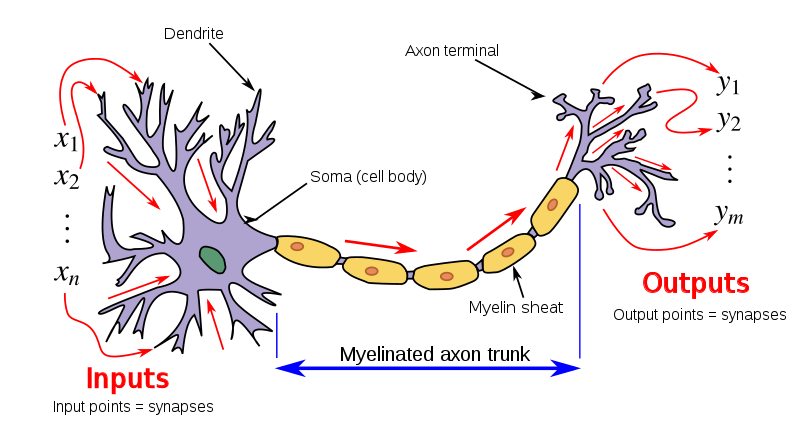
\includegraphics[width=0.55\linewidth]{\toplevelprefix/chapters/chapter1/figs/neuron.png} \hspace{3mm}
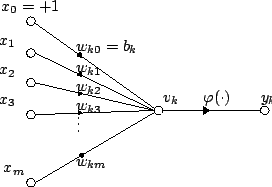
\includegraphics[width=0.40\linewidth]{\toplevelprefix/chapters/chapter1/figs/Artificial_neuron.png}
    \caption{Primul model matematic al unui neuron artificial (dreapta) care emulează modul în care un neuron (stânga) procesează semnale.}
    \label{fig:neuron}
\end{figure}

Inspirat de sistemul nervos din creier, modelul matematic al primului neuron artificial\footnote{cunoscut ca Unitatea de Prag Liniar sau un perceptron.} a fost propus de Warren McCulloch\footnote{Un profesor de psihiatrie la Universitatea din Chicago la acea vreme} și Walter Pitts în 1943 \cite{McCulloch-Pitts}. Acesta descrie relația dintre intrarea $x_i$ și ieșirea $o_j$ ca:
\begin{equation}
    o_j = \varphi\Big( \sum_i w_{ji}x_i\Big),
\end{equation}
unde $\varphi(\cdot)$ este o anumită activare neliniară, modelată în mod normal de o funcție de prag. Acest model este ilustrat în \Cref{fig:neuron}. După cum putem vedea, această formă împărtășește deja caracteristicile principale ale unei unități de bază în rețelele neuronale profunde moderne. Modelul este derivat din observații despre cum funcționează un singur neuron în sistemul nostru nervos. Cu toate acestea, oamenii nu știau exact ce funcții dorește să realizeze și să efectueze o colecție de astfel de neuroni. La un nivel mai tehnic, nici nu erau siguri ce funcție de activare neliniară $\varphi(\cdot)$ ar trebui folosită. Prin urmare, istoric au fost propuse multe variante.\footnote{Funcție treaptă, pragare dură sau moale, Unitate Liniară Rectificată (ReLU), sigmoid etc.}

\begin{figure}[t]
\centering
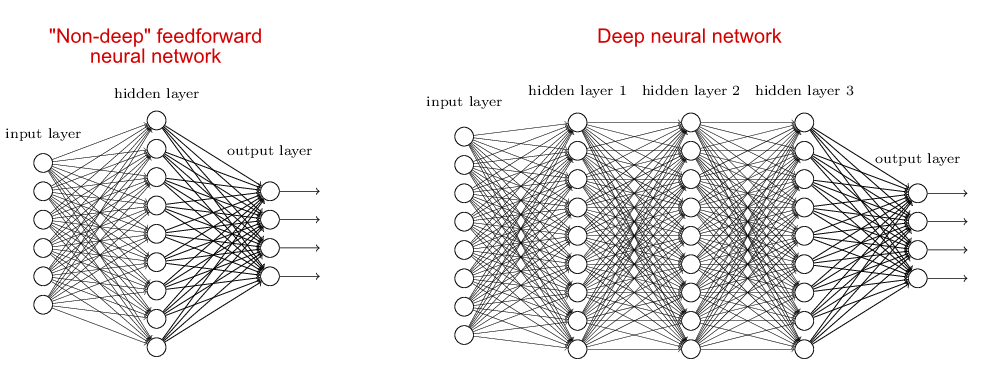
\includegraphics[width=0.85\linewidth]{\toplevelprefix/chapters/chapter1/figs/single-deep.png}
    \caption{O rețea cu un singur strat ascuns (stânga) versus o rețea profundă (dreapta).}
    \label{fig:single-deep}
\end{figure}
\paragraph{Rețea neuronală artificială.}
În anii 1950, Frank Rosenblatt a fost primul care a construit o mașină cu o {\em rețea} de astfel de neuroni artificiali, prezentată în \Cref{fig:perceptron}. Mașina se numește Mark I Perceptron, care constă dintr-un strat de intrare, un strat de ieșire și un singur strat ascuns format din 512 neuroni artificiali, așa cum se arată în \Cref{fig:perceptron} stânga, care este similar cu ceea ce este ilustrat în \Cref{fig:single-deep} stânga. A fost concepută pentru a clasifica imagini optice de litere. Cu toate acestea, capacitatea unei rețele cu un singur strat este limitată și poate învăța doar tipare separabile liniar. Într-o carte din 1969 {\em Perceptrons: O Introducere în Geometria Computațională} de Marvin Minsky și Seymour Papert \cite{Minsky-1969}, s-a arătat că arhitectura cu un singur strat a Mark I Perceptron nu poate învăța o funcție XOR. Acest rezultat a diminuat semnificativ interesul oamenilor pentru rețelele neuronale artificiale, chiar dacă s-a dovedit ulterior că o rețea cu mai multe straturi este capabilă să învețe o funcție XOR \cite{Rumelhart1986}. De fapt, o rețea multi-strat (suficient de mare), așa cum se arată în \Cref{fig:single-deep} dreapta, constând din astfel de neuroni simpli poate simula orice mașină cu stare finită, chiar și mașina Turing universală.\footnote{Nu confundați ce sunt capabile să facă rețelele neuronale în principiu cu dacă este tractabil sau ușor să învățați o rețea neuronală care realizează anumite funcții dorite.} Cu toate acestea, ulterior, studiul rețelelor neuronale artificiale a intrat în prima sa iarnă în anii 1970.

\begin{figure}
    \centering
    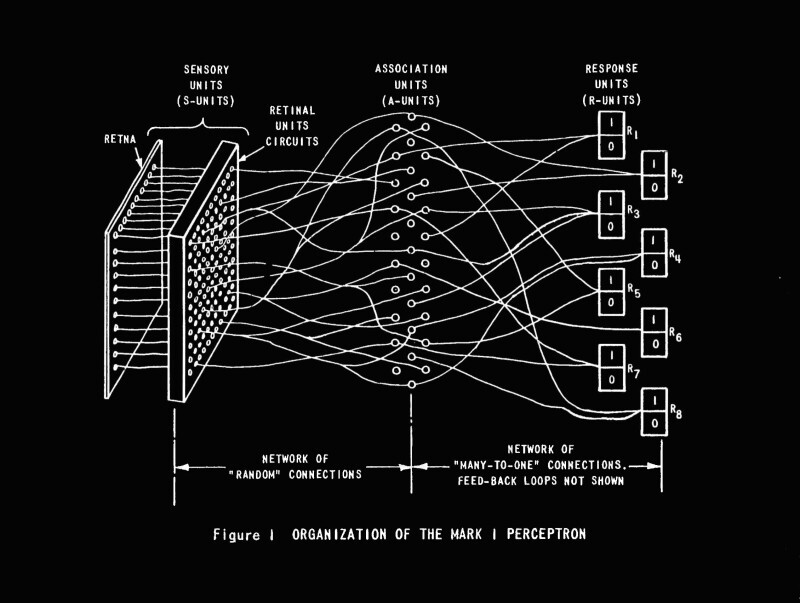
\includegraphics[width=0.45\linewidth]{\toplevelprefix/chapters/chapter1/figs/visu-large.jpg}
    \hspace{2mm} 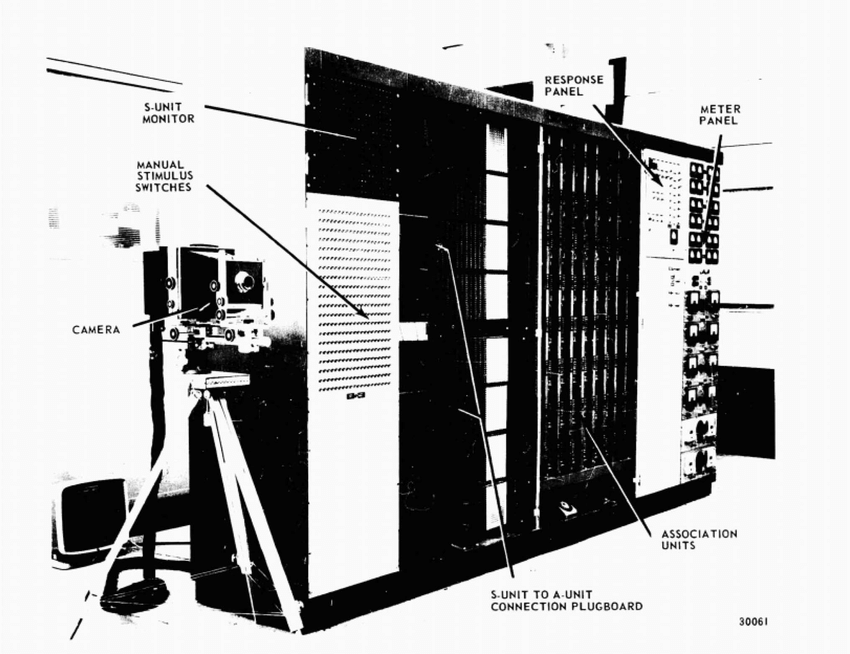
\includegraphics[width=0.45\linewidth]{\toplevelprefix/chapters/chapter1/figs/Original-Mark-I-perceptron-as-seen-in-its-operators-manual-20.ppm.png}
    \caption{Mașina Mark I Perceptron dezvoltată de Frank Rosenblatt la sfârșitul anilor 1950.}
    \label{fig:perceptron}
\end{figure}


\paragraph{Rețele neuronale convoluționale.}
Experimentarea oarecum dezamăgitoare timpurie cu rețele neuronale artificiale precum Mark I Perceptron în anii 50 și 60 a sugerat că s-ar putea să nu fie suficient să conectăm pur și simplu neuronii într-o manieră generală ca perceptroni multistrat (MLP). Pentru a construi rețele efective și eficiente, trebuie să înțelegem ce scop sau funcție trebuie să realizeze neuronii într-o rețea în mod colectiv, astfel încât aceștia să fie organizați și învățați într-un anumit mod special. Din nou, studiul inteligenței mașinilor s-a întors la a trage inspirație din modul în care funcționează sistemul nervos al animalelor.

Se știe că cea mai mare parte a creierului nostru este dedicată procesării informațiilor vizuale. În anii 1950 și 1960, David Hubel și Torsten Wiesel au studiat sistematic cortexurile vizuale ale pisicilor. S-a descoperit că cortexul vizual conține diferite tipuri de celule (cunoscute ca celule simple și celule complexe), care sunt sensibile la stimuli vizuali de diferite orientări și locații \cite{Hubel-Wiesel-1959}. Hubel și Wiesel au câștigat Premiul Nobel pentru Fiziologie sau Medicină în 1981 pentru descoperirea lor revoluționară.


Pe partea rețelelor neuronale artificiale, lucrarea lui Hubel și Wiesel l-a inspirat pe Kunihiko Fukushima care a proiectat rețeaua „neocognitron" în 1980, care constă din neuroni artificiali care emulează neuronii biologici din cortexurile vizuale \cite{Fukushima1980NeocognitronAS}. Aceasta este cunoscută ca prima {\em rețea neuronală convoluțională} (CNN), iar arhitectura sa este ilustrată în \Cref{fig:neocognitron}. Spre deosebire de perceptron, neocognitronul avea mai mult de un strat ascuns și putea fi văzut ca o rețea profundă, așa cum este comparat în \Cref{fig:single-deep} dreapta.

De asemenea, inspirat de modul în care funcționează neuronii în cortexul vizual al pisicii, el a fost și primul care a introdus utilizarea {\em unității liniare rectificate} (ReLU):
\begin{equation}
    \varphi(x) = \max\{0, x\} = \casework{x, & \text{dacă} \, x > 0, \\ 0, \quad & \text{dacă} \, x \leq 0,}
\end{equation}
pentru funcția de activare $\varphi(\cdot)$ în 1969 \cite{Fukushima-1969}. Dar abia în anii recenți ReLU a devenit o funcție de activare larg utilizată în rețelele neuronale (convoluționale) profunde moderne. Vom învăța din această carte de ce aceasta este o alegere bună odată ce explicăm operațiile principale pe care rețelele profunde încearcă să le implementeze: compresia.

\begin{figure}
    \centering
    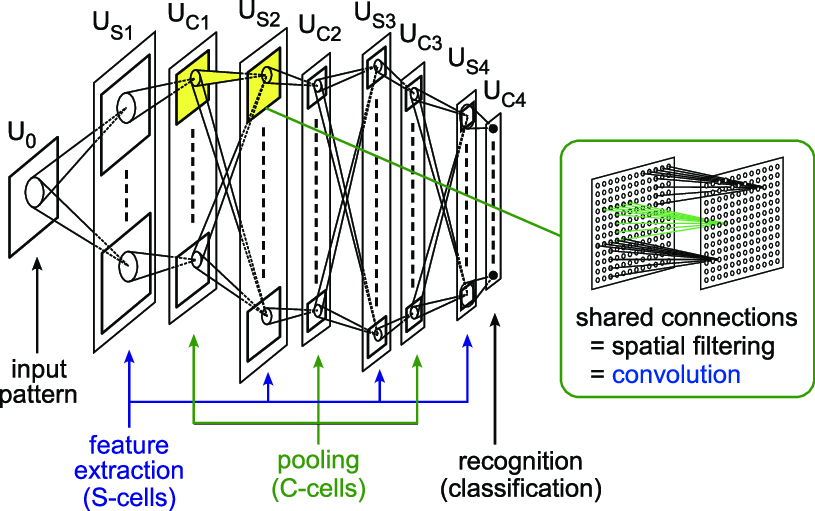
\includegraphics[width=0.6\linewidth]{\toplevelprefix/chapters/chapter1/figs/neocognitron.png}
    \caption{Originea rețelelor neuronale convoluționale: Neocognitronul de Kunihiko Fukushima în 1980. Observați că straturile intercalate de convoluții și pooling încearcă să emuleze funcțiile celulelor simple și ale celulelor complexe descoperite în cortexurile vizuale ale pisicilor.}
    \label{fig:neocognitron}
\end{figure}

Rețelele de tip CNN au continuat să evolueze în anii 1980 și au fost introduse și studiate multe variante diferite. Cu toate acestea, în ciuda capacităților remarcabile ale rețelelor profunde și a arhitecturilor îmbunătățite inspirate de neuroștiință, a rămas extrem de dificil să antrenăm astfel de rețele profunde pentru o sarcină reală precum clasificarea imaginilor. Cum să faci o rețea să funcționeze depindea de multe euristici și trucuri inexplicabile care au limitat cu adevărat atractivitatea și aplicabilitatea rețelelor neuronale. O descoperire majoră a venit în jurul anului 1989 când Yann LeCun a folosit cu succes {\em propagarea înapoi} (BP) pentru a învăța o rețea neuronală convoluțională profundă pentru recunoașterea cifrelor scrise de mână \cite{LeCun-1989}, cunoscută mai târziu sub numele de LeNet (vezi \Cref{fig:LeNet-5}). După câțiva ani de dezvoltare persistentă, perseverența sa a dat roade: performanța LeNet a devenit în cele din urmă suficient de bună pentru utilizare practică la sfârșitul anilor 1990 \cite{LeCun-1998}: a fost folosită de Poșta SUA pentru recunoașterea cifrelor scrise de mână (pentru codurile poștale). LeNet a fost considerat rețeaua „prototip" pentru toate rețelele neuronale profunde moderne, cum ar fi AlexNet și ResNet, pe care le vom discuta mai târziu. Datorită acestei lucrări, Yann LeCun a primit Premiul Turing 2018.\footnote{Împreună cu alți doi pionieri ai rețelelor profunde, Yoshua Bengio și Geoffrey Hinton.}

\begin{figure}
    \centering
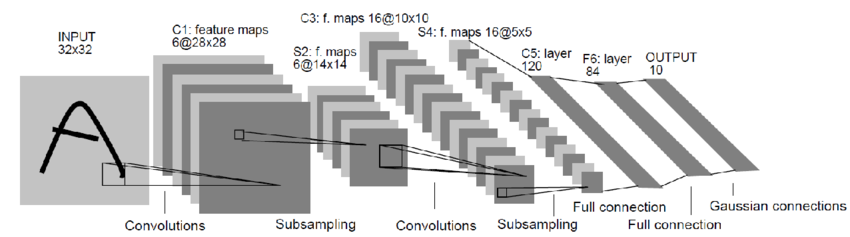
\includegraphics[width=0.95\linewidth]{\toplevelprefix/chapters/chapter1/figs/LeNet-5.png}
    \caption{Rețeaua neuronală convoluțională LeNet-5 proiectată de Yann LeCun în 1989.}
    \label{fig:LeNet-5}
\end{figure}

\paragraph{Propagarea înapoi.}
În istorie, soarta rețelelor neuronale profunde pare să fie strâns legată de cum pot fi antrenate ușor și eficient. Propagarea înapoi (BP) a fost introdusă din acest motiv. Știm că un perceptron cu straturi multiple poate fi exprimat ca o compoziție a unei secvențe de mapări liniare și activări neliniare după cum urmează:
\begin{equation}
h(\bm W_1, \ldots, \bm W_L) = f^L(\bm W_Lf^{L-1}(\bm W_{L-1} \cdots f^2(\bm W_2f^1(\bm W_1\x)))).
\end{equation}
Pentru a antrena ponderile rețelei $\{\bm W_l\}_{l=1}^L$ pentru a reduce eroarea de predicție/clasificare pe baza unui algoritm de coborâre pe gradient, trebuie să evaluăm gradientul ${\partial h}/{\partial \bm W_l}$. Este bine cunoscut, din {\em regula lanțului} din calcul, că gradienții pot fi calculați eficient pentru acest tip de funcții, cunoscut mai târziu ca propagare înapoi (BP). Vezi \Cref{app:optimization} pentru o descriere detaliată. Tehnica propagării înapoi era deja cunoscută și practicată de oameni în domenii precum controlul optim și programarea dinamică în anii 1960 și 1970. De exemplu, a apărut în teza de doctorat din 1974 a Dr. Paul Werbos \cite{Werbos-1974, Werbos1994TheRO}. În 1986, David Rumelhart și colab. au fost primii care au aplicat propagarea înapoi pentru a antrena o rețea cu perceptron multistrat (MLP) \cite{Rumelhart1986}. De atunci, BP a devenit din ce în ce mai popular deoarece oferă un algoritm {\em scalabil} pentru a învăța rețele neuronale profunde mari.\footnote{deoarece poate fi implementat eficient pe platforme de calcul care facilitează calculul paralel și distribuit.} Este acum o tehnică aproape dominantă pentru antrenarea rețelelor neuronale profunde astăzi. Cu toate acestea, se crede că natura nu învață prin propagare înapoi, deoarece un astfel de mecanism este încă mult prea costisitor pentru implementarea fizică de către natură\footnote{După cum am discutat mai devreme, natura învață aproape omniprezent să corecteze erorile prin feedback în buclă închisă.}. Acest lucru lasă evident un spațiu enorm pentru îmbunătățiri în viitor, așa cum vom discuta mai mult.

Cu toate acestea, în ciuda progresului algoritmic de mai sus și a practicii promițătoare din anii 1980, antrenarea rețelelor neuronale profunde a rămas extrem de capricioasă și costisitoare pentru sistemele de calcul din anii 1980 și 1990. La sfârșitul anilor 1990, mașinile cu vectori suport (SVM) \cite{SVM-1995} au devenit foarte populare deoarece erau văzute ca o alternativă mai bună la rețelele neuronale pentru sarcini precum clasificarea.\footnote{De fapt, idei similare pentru a rezolva probleme de clasificare pot fi urmărite înapoi la lucrarea de disertație de doctorat a lui Thomas Cover, care a fost condensată și publicată într-o lucrare în 1964 \cite{Cover-1964}.} Existau două motive principale: în primul rând, SVM se baza pe un cadru riguros de învățare statistică cunoscut sub numele de teoria Vapnik-Chervonenkis (VC); și în al doilea rând, duce la algoritmi destul de eficienți bazați pe optimizare convexă \cite{BoydVa04}. Ascensiunea SVM a adus o a doua iarnă studiului rețelelor neuronale în jurul începutului anilor 2000.

\paragraph{Autocodare compresivă.}
La sfârșitul anilor 1980 și 1990, rețelele neuronale artificiale au fost deja adoptate pentru a învăța reprezentări cu dimensiuni reduse ale datelor cu dimensiuni mari, cum ar fi imaginile. S-a arătat că rețelele neuronale pot fi folosite pentru a învăța PCA din date \cite{Oja1982SimplifiedNM,Baldi89}, în loc să folosească metodele clasice discutate în \Cref{sec:PCA-ICA}. S-a argumentat, de asemenea, la sfârșitul anilor 1980 că, datorită capacității sale de a modela transformări neliniare, rețelele neuronale au fost sugerate pentru a învăța reprezentări cu dimensiuni reduse pentru date cu distribuții neliniare. Similar cu cazul PCA liniar, se poate încerca să învețe simultan un codificator neliniar de reducere a dimensionalității $f$ și un decodificator $g$, fiecare modelat de o rețea neuronală profundă \cite{Rumelhart1986,Kramer1991NonlinearPC}:
\begin{equation}
    \X   \xrightarrow{\hspace{2mm} f \hspace{2mm}} \Z  \xrightarrow{\hspace{2mm} g \hspace{2mm}} \hat \X.
       \label{eqn:auto-encoding-deep-networks}
\end{equation}
Prin impunerea ca datele decodate $\hat \X$ să fie consistente cu originalul $\X$, să zicem prin minimizarea unei erori de reconstrucție de tip MMSE\footnote{Deși erorile de tip MMSE sunt cunoscute ca fiind problematice pentru datele imagistice care au structuri neliniare complexe. După cum vom discuta curând, o mare parte din munca recentă în metodele generative, inclusiv GAN-urile, a fost pentru a găsi înlocuitori ai funcțiilor de distanță mai bune între datele originale $\X$ și cele regenerate $\hat \X$.}:
\begin{equation}
    \min_{f,g} \big\|\X - \hat \X\big\|_2^2 = \big\|\X - g(f( \X))\big\|_2^2,
\end{equation}
un autocodor poate fi învățat din datele $\X$ însele.

Dar cum putem garanta că o astfel de autocodare captează într-adevăr structurile adevărate cu dimensiuni reduse din $\X$ în loc să dea o reprezentare redundantă trivială? De exemplu, putem alege pur și simplu $f$ și $g$ să fie maparea identitate și $\Z = \X$. Deci, pentru a asigura că autocodarea merită, se dorește ca reprezentarea rezultată să fie compresivă, în termenii unei anumite măsuri calculabile de complexitate. În 1993, Geoffrey Hinton și colegii au propus să folosească lungimea de codare ca o astfel de măsură, prin urmare obiectivul autocodării a devenit să găsească o astfel de reprezentare care minimizează lungimea de codare \cite{Hinton-1993}. Această lucrare a stabilit, de asemenea, o conexiune fundamentală între principiul lungimii minime de descriere \cite{Rissanen-1978} și minimizarea energiei libere (Helmholtz). Lucrarea ulterioară \cite{Hinton504} din grupul lui Hinton a arătat empiric că o astfel de autocodare este capabilă să învețe reprezentări semnificative cu dimensiuni reduse pentru imagini din lumea reală. Un sondaj mai cuprinzător al autocodorilor a fost făcut de Pierre Baldi în 2011 \cite{Baldi2011}, chiar înainte ca rețelele profunde să devină populare. Vom discuta mai multe despre măsura complexității și autocodare mai târziu în \Cref{sec:unifying-approach} și vom oferi un studiu sistematic al autocodării compresive în \Cref{ch:consistent}, cu o viziune mai unificatoare.


\begin{figure}
    \centering
    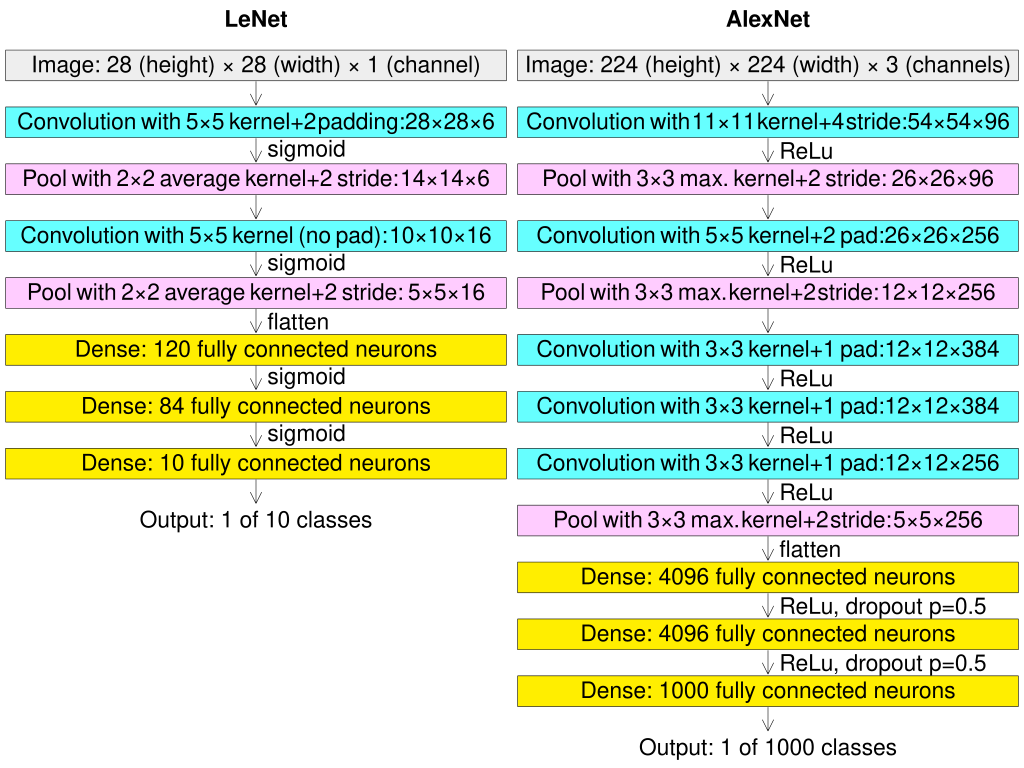
\includegraphics[width=0.8\linewidth]{\toplevelprefix/chapters/chapter1/figs/Comparison_image_neural_networks.svg.png}
    \caption{Arhitectura LeNet \cite{LeCun-1989} versus cea a AlexNet \cite{krizhevsky2012imagenet}.}
    \label{fig:LeNet-AlexNet}
\end{figure}


\subsubsection{Rețele Neuronale Profunde Moderne}
Timp de aproape 30 de ani, din anii 1980 până în anii 2010, pentru studiul învățării automate și al inteligenței mașinilor, rețelele neuronale nu au fost considerate serios de mainstream. Rețelele neuronale (profunde) timpurii, cum ar fi LeNet, au arătat performanțe promițătoare pentru probleme de clasificare la scară mică, cum ar fi recunoașterea cifrelor. Cu toate acestea, proiectarea și practica rețelelor erau destul de empirice, seturile de date disponibile la acea vreme erau mici, iar algoritmul BP era o povară computațională uriașă pentru calculatoarele de atunci. Acești factori au dus la lipsa de interes pentru rețelele neuronale, iar progresul a stagnat, cu doar o mână de cercetători lucrând la ele.

\paragraph{Clasificare și recunoaștere.}
După cum se dovedește, potențialul enorm al rețelelor neuronale profunde putea fi eliberat doar odată ce există suficiente date și putere de calcul. Avansând rapid până în anii 2010, seturi de date mult mai mari, cum ar fi ImageNet, au devenit disponibile, iar GPU-urile au devenit suficient de puternice pentru a face BP mult mai accesibil, chiar și pentru rețele mult mai mari decât LeNet. În jurul anului 2012, o rețea neuronală convoluțională profundă cunoscută sub numele de AlexNet a atras atenția, deoarece a depășit metodele de clasificare existente cu o marjă semnificativă cu setul de date ImageNet \cite{krizhevsky2012imagenet}.\footnote{De fapt, înainte de aceasta, rețelele profunde au demonstrat performanțe de ultimă generație în sarcinile de recunoaștere a vorbirii. Dar nu au primit atâta atenție până la succesul lor cu clasificarea imaginilor.} \Cref{fig:LeNet-AlexNet} arată comparația dintre AlexNet și LeNet. AlexNet împărtășește multe caracteristici comune cu LeNet, doar că este mai mare și a adoptat ReLU ca activare neliniară în loc de funcția Sigmoid folosită în LeNet. Parțial datorită influenței acestei lucrări, Geoffrey Hinton a primit Premiul Turing 2018.


Acest succes timpuriu a inspirat comunitatea inteligenței mașinilor, în următorii câțiva ani, să exploreze noi variații și îmbunătățiri ale designului rețelei. În special, oamenii au descoperit empiric că cu cât rețelele sunt mai mari și mai profunde, cu atât performanța este mai bună în sarcini precum clasificarea imaginilor. Au fost încercate, testate și popularizate multe arhitecturi de rețele profunde. Câteva notabile includ VGG \cite{Simonyan15}, GoogLeNet \cite{Szegedy2014GoingDW}, ResNet \cite{He2016-lc} și mai recent Transformers \cite{vaswani2017attention} etc. În ciuda progresului rapid în performanța empirică, a existat o lipsă de explicație teoretică pentru aceste arhitecturi descoperite empiric, inclusiv relațiile dintre ele, dacă există. Un scop al acestei cărți este să dezvăluie ce obiectiv comun pot servi toate aceste rețele și de ce împărtășesc anumite caracteristici comune, inclusiv straturi multiple de operator liniar intercalate cu activare neliniară (vezi \Cref{ch:representation}).

\paragraph{Învățare prin întărire.}
Succesele timpurii ale rețelelor profunde au fost în principal pentru sarcini de clasificare într-un cadru de învățare supravegheată, cum ar fi recunoașterea vorbirii și recunoașterea imaginilor. Rețelele profunde au fost adoptate ulterior de echipa DeepMind, condusă de Demis Hassabis, pentru a învăța politici de luare a deciziilor sau control pentru jocuri. În acest context, rețelele profunde sunt folosite pentru a modela politica optimă de decizie/control sau funcția de valoare optimă asociată, așa cum se arată în \Cref{fig:Alpha-Go}. Acești parametri de rețea sunt optimizați incremental\footnote{Să zicem pe baza propagării înapoi (BP).} pe baza recompensei returnate din succesul sau eșecul jocului cu politica actuală. Această metodă de învățare este denumită în general {\em învățare prin întărire} \cite{Sutton-Barto}, originată din practica sistemelor de control la sfârșitul anilor 1960 \cite{Waltz1965AHA,Mendel1970ReinforcementlearningCA}. Rădăcinile sale anterioare pot fi urmărite înapoi la o istorie mult mai lungă și mai bogată a {\em programării dinamice} de Richard Bellman \cite{Bellman-DP} și {\em învățării prin încercare și eroare} de Marvin Minsky \cite{Minsky-1954} în anii 1950.

Din perspectivă de implementare, combinația dintre rețelele profunde și învățarea prin întărire s-a dovedit a fi destul de puternică: rețelele profunde pot fi folosite pentru a aproxima politica de control și funcția de valoare pentru medii din lumea reală care sunt dificil de modelat analitic. Această practică a condus în cele din urmă la sistemul AlphaGo, dezvoltat de compania DeepMind, care a surprins lumea în 2016 învingând un jucător uman de top Lee Sedol în jocul Go și apoi pe campionul mondial Ke Jie în 2017.\footnote{În 1996, sistemul Deep Blue al IBM a făcut istorie învingându-l pe marele maestru rus Garry Kasparov la șah. A folosit în principal tehnici tradiționale de învățare automată, cum ar fi căutarea în arbore și tăierea, care nu erau atât de scalabile și nu s-au dovedit de succes pentru jocuri mai provocatoare precum Go timp de peste 20 de ani.}

Succesul AlphaGo a venit ca o mare surpriză pentru societatea de calcul care crede în general că spațiul de stare pentru căutare este prea prohibitiv de mare pentru a admite orice soluție eficientă, în termeni de calcul și dimensiunea eșantionului. Singura explicație rezonabilă pentru succesul său este că trebuie să existe structuri foarte bune în funcția optimă de valoare/politică a jocului Go. Dimensiunea lor intrinsecă nu este atât de mare și pot fi aproximate bine de o rețea neuronală, învățabilă din nu atât de prohibitiv multe eșantioane.

\begin{figure}
    \centering
    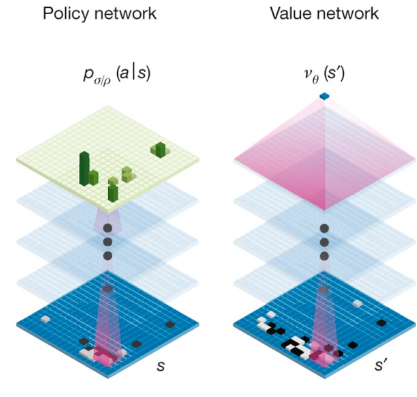
\includegraphics[width=0.5\linewidth]{\toplevelprefix/chapters/chapter1/figs/Policy-Value.png}
    \caption{AlphaGo: Folosirea rețelelor neuronale profunde pentru a modela politica optimă sau funcția de valoare optimă pentru jocul Go.}
    \label{fig:Alpha-Go}
\end{figure}

\paragraph{Generare și predicție.}
Se poate vedea practicile timpurii ale rețelelor profunde din anii 2010 ca fiind concentrate mai mult pe extragerea informațiilor relevante din datele $\X$ și codificarea lor pentru o anumită reprezentare specifică sarcinii $\Z$ (să zicem că $\Z$ reprezintă etichete de clasă în sarcinile de clasificare):
\begin{equation}
    \X   \xrightarrow{\hspace{2mm} f \hspace{2mm}} \Z.
       \label{eqn:encoding-deep-networks}
\end{equation}
În această setare, maparea $f$ care trebuie învățată nu trebuie să păstreze majoritatea informațiilor distribuite despre $\X$, ci doar statisticile suficiente necesare pentru o sarcină specifică. De exemplu, un eșantion $\x$ din $\X$ ar putea fi o imagine a unui măr, care este mapată de $f$ la eticheta sa de clasă $\z =$ „măr". {\em Cadrul gâtului de sticlă informațional} \cite{Tishby-ITW2015} a fost propus în 2015 pentru a analiza rolul rețelelor profunde într-un astfel de context.

Cu toate acestea, în multe situații moderne, cum ar fi cele numite modele mari de fundație, oamenii trebuie adesea să decodeze $\Z$ pentru a recupera $\X$ corespunzător cu un anumit grad de precizie:
\begin{equation}
    \Z   \xrightarrow{\hspace{2mm} g  \hspace{2mm}} \hat \X.
       \label{eqn:decoding-deep-networks}
\end{equation}
Deoarece $\X$ reprezintă de obicei date observate din lumea externă, un decodificator bun ne-ar permite să simulăm sau să prezicem ce se întâmplă în lume. De exemplu, într-o sarcină „text la imagine" sau „text la video", $\z$ reprezintă în mod normal textele care descriu conținutul unei imagini dorite $\x$. Decodificatorul ar trebui să poată genera un $\hat \x$ care are același conținut ca $\x$. De exemplu, dată fiind o clasă de obiecte $\z = $ „măr", decodificatorul $g$ ar trebui să genereze o imagine $\hat \x$ care arată ca un măr, deși nu neapărat exact la fel ca originalul $\x$.



\paragraph{Generare prin abordări discriminative.}
Pentru ca imaginile generate $\hat \X$ să fie similare cu imaginile naturale adevărate $\X$, trebuie să putem evalua și minimiza o anumită distanță:
\begin{equation}
    \min d(\X, \hat \X).
\end{equation}
După cum se dovedește, majoritatea distanțelor motivate teoretic sunt extrem de dificile, dacă nu imposibile, de calculat și optimizat pentru distribuții în spațiu cu dimensiuni mari dar cu dimensiune intrinsecă mică.\footnote{Acesta este cazul chiar dacă este dată o familie parametrică de distribuție pentru $\X$. Distanța devine adesea prost condiționată sau prost definită pentru distribuții cu suporturi cu dimensiuni reduse. Ceea ce ar putea fi și mai rău este că familia aleasă ar putea să nu poată aproxima bine distribuția adevărată de interes.}

În 2007, Zhuowen Tu, un fost student al lui Song-Chun Zhu, probabil dezamăgit de încercările analitice timpurii de a modela și genera imagini naturale (discutate mai devreme), a decis să încerce o abordare drastic diferită. Într-o lucrare publicată în CVPR 2007 \cite{Tu-2007}, el a fost primul care a sugerat că se poate învăța un model generativ pentru imagini printr-o abordare discriminativă. Ideea este simplă: dacă este dificil să evaluezi distanța $d(\X, \hat \X)$, ai putea încerca să înveți un discriminator $d$ pentru a separa $\hat \X$ de $\X$:
\begin{equation}
    \Z   \xrightarrow{\hspace{2mm} g  \hspace{2mm}} \hat \X, \X \xrightarrow{\hspace{2mm} d  \hspace{2mm}} \boldsymbol{0}, \boldsymbol{1},
       \label{eqn:gan-networks}
\end{equation}
unde $\boldsymbol{0}, \boldsymbol{1}$ indică dacă o imagine este generată sau nu.
Intuitiv, cu cât este mai greu să separăm $\hat \X$ și $\X$, probabil cu atât sunt mai aproape.

Lucrarea lui Tu \cite{Tu-2007} a fost prima care a demonstrat fezabilitatea învățării unui model generativ dintr-o abordare discriminativă. Cu toate acestea, lucrarea a adoptat metode tradiționale pentru a genera imagini și a clasifica distribuții (cum ar fi boosting), și erau lente și greu de implementat. După 2012, rețelele neuronale profunde au devenit foarte populare pentru clasificarea imaginilor. În 2014, Ian Goodfellow și colegii au propus din nou să genereze imagini naturale cu o abordare discriminativă \cite{Goodfellow-2014}. Ei au sugerat să folosească rețele neuronale profunde pentru a modela generatorul $g$ și discriminatorul $d$ în schimb. Mai mult, au propus să învețe generatorul $g$ și discriminatorul $d$ printr-un joc minimax:
\begin{equation}
    \min_g \max_d \ell(\X, \hat \X),
\end{equation}
unde $\ell(\cdot)$ este o anumită funcție de pierdere naturală asociată cu clasificarea. În cuvinte, discriminatorul $d$ încearcă să maximizeze succesul său în separarea $\X$ și $\hat \X$, în timp ce generatorul $g$ încearcă să facă opusul. Din acest motiv, această abordare este numită {\em rețele generative adversariale} (GAN). S-a arătat că odată antrenate pe un set de date mare, GAN-urile pot genera într-adevăr imagini foto-realiste. Parțial datorită influenței acestei lucrări, Yoshua Bengio a primit Premiul Turing 2018.

Abordarea discriminativă pare să fie o modalitate destul de inteligentă de a ocoli o dificultate fundamentală în învățarea distribuției. Cu toate acestea, riguros vorbind, această abordare nu rezolvă pe deplin această dificultate fundamentală deloc. Este arătat de \cite{Goodfellow-2014} că, cu o pierdere aleasă corespunzător, formularea minimax este matematic echivalentă cu minimizarea {\em distanței Jensen-Shannon} (vezi \cite{Cover-Thomas}) între $\X$ și $\hat \X$. Aceasta este cunoscută ca fiind o problemă dificilă pentru două distribuții cu dimensiuni reduse într-un spațiu cu dimensiuni mari. Ca rezultat, în practică, GAN-urile se bazează de obicei pe multe euristici și trucuri inginerești și suferă adesea de probleme de instabilitate, cum ar fi {\em colapsul modului}.\footnote{Cu toate acestea, o astfel de formulare minimax oferă o aproximare practică a distanței. Simplifică implementarea și evită anumite capcane în calcularea directă a distanței.} În general, a existat o lipsă de îndrumare teoretică cu privire la modul de îmbunătățire a practicii GAN-urilor.

\paragraph{Generare prin îndepărtarea zgomotului și difuzie.}
În 2015, la scurt timp după ce GAN a fost introdus și a devenit popular, Surya Ganguli și studenții săi și-au dat seama și au sugerat că un proces iterativ de îndepărtare a zgomotului modelat de o rețea profundă poate fi folosit pentru a învăța o distribuție generală, cum ar fi cea a imaginilor naturale \cite{Sohl-Dickstein2015}. Metoda lor a fost inspirată de proprietățile proceselor speciale gaussiene și binomiale, studiate de William Feller încă din 1949 \cite{Feller1949OnTT}.\footnote{Din nou, în era magică a anilor 1940!}

\begin{figure}[t]
    \centering
    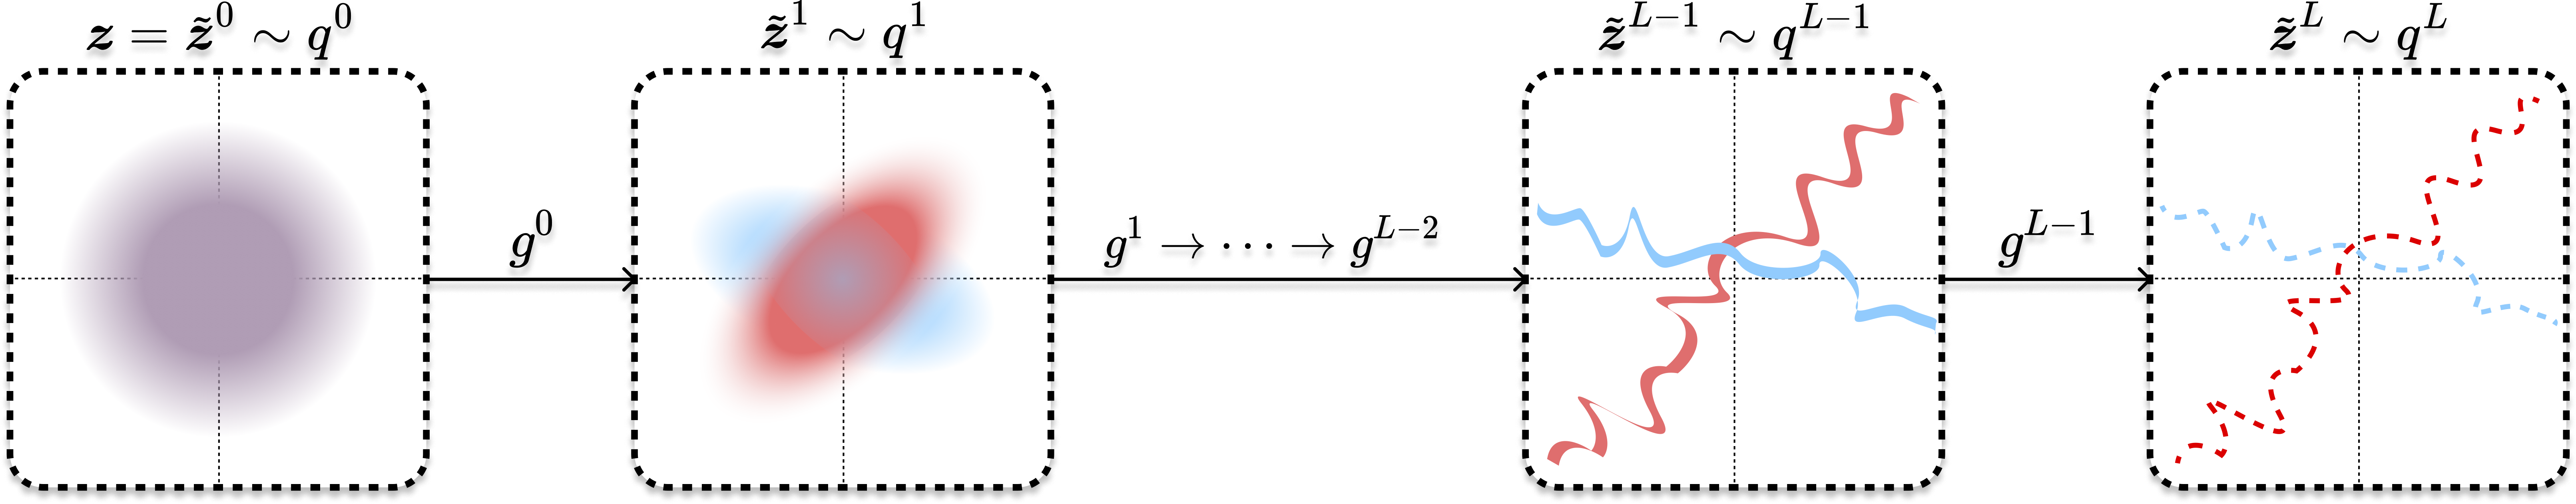
\includegraphics[width=\linewidth]{\toplevelprefix/chapters/chapter1/figs/diffusion_pipeline.png}
    \caption{Ilustrarea unui proces iterativ de îndepărtare a zgomotului și compresie care, pornind de la o distribuție gaussiană $q^0 = \mathcal{N}(\boldsymbol{0}, \boldsymbol{I})$, converge la o distribuție arbitrară de date cu dimensiuni reduse $q^L = p(\x)$.}
    \label{fig:diffusion}
\end{figure}

Curând, operatorii de îndepărtare a zgomotului bazați pe funcția de scor \cite{hyvarinen05a}, introduși pe scurt în Secțiunea \ref{sec:denoising-intro}, s-au dovedit a fi mai generali și au unificat procesele și algoritmii de îndepărtare a zgomotului și difuzie \cite{song2019,song2020score,ho2020denoising}. Figura \ref{fig:diffusion} oferă o ilustrare a procesului care transformă o distribuție gaussiană generică $q^0 = \mathcal{N}(\boldsymbol{0}, \boldsymbol{I})$ într-o distribuție empirică (arbitrară) $p(\x)$ prin efectuarea unei secvențe de operații iterative de îndepărtare a zgomotului (sau compresie):
\begin{equation}
        \z^0 \sim  \mathcal{N}(\boldsymbol{0}, \boldsymbol{I})\xrightarrow{\hspace{2mm} g^0  \hspace{2mm}} \z^1 \xrightarrow{\hspace{2mm} g^1 \hspace{2mm}} \cdots \xrightarrow{\hspace{2mm} g^{L-1}  \hspace{2mm}} \z^L \sim p(\x).
\end{equation}
Până acum, îndepărtarea zgomotului (și difuzia) au înlocuit GAN-urile și au devenit o metodă principală pentru învățarea distribuțiilor imaginilor și videoclipurilor, ducând la motoare comerciale populare de generare a imaginilor, cum ar fi Midjourney și Stability.ai.
În \Cref{ch:compression} vom introduce și studia sistematic metoda de îndepărtare a zgomotului și difuzie pentru învățarea unei distribuții generale cu dimensiuni reduse.



\section{O Abordare Unificatoare}\label{sec:unifying-approach}
Până acum, am oferit o relatare scurtă a obiectivului principal și istoriei inteligenței mașinilor și multe idei și abordări importante asociate cu aceasta. În ultimii ani, după succesul empiric al rețelelor neuronale profunde, au fost depuse eforturi enorme pentru a dezvolta cadre teoretice care să ne ajute să înțelegem toate rețelele neuronale profunde proiectate empiric, fie anumite componente aparent necesare (de exemplu, dropout, normalizare, atenție etc.) sau comportamentele lor generale (de exemplu, dublă coborâre, colaps neuronal etc.).

Parțial motivată de aceasta, această carte își propune să atingă mai multe obiective importante și provocatoare:
\begin{itemize}
    \item Dezvoltarea unui cadru teoretic care ne-ar permite să derivăm interpretarea matematică riguroasă a rețelelor neuronale profunde.
    \item Asigurarea corectitudinii distribuției de date învățate și consistenței cu reprezentarea învățată.
    \item Demonstrarea că cadrul poate duce la arhitecturi performante și poate ghida îmbunătățiri suplimentare în practică.
\end{itemize}
În ultimii câțiva ani, există dovezi din ce în ce mai multe că aceste obiective pot fi într-adevăr atinse, valorificând teoria și soluțiile modelelor analitice clasice cu dimensiuni reduse discutate pe scurt mai devreme (mai amănunțit în \Cref{ch:classic}) și integrând idei fundamentale din câteva domenii conexe, și anume teoria informației/codării, teoria controlului/jocurilor și optimizarea. Această carte își propune să ofere o introducere sistematică în această nouă abordare.

\subsection{Învățarea Reprezentărilor Parcimonioase}
\label{sec:computational-approach-compression}
O condiție necesară pentru ca orice sarcină de învățare să fie posibilă este ca secvențele de interes să fie {\em calculabile}, cel puțin în sensul lui Alan Turing \cite{Turing-1936}. Adică, o secvență poate fi calculată printr-un program pe un computer tipic.\footnote{Există într-adevăr secvențe bine definite care nu sunt calculabile.} Pe lângă faptul de a fi calculabile, cerem ca calculul să fie {\em tractabil}.\footnote{Nu trebuie să luăm în considerare prezicerea lucrurilor a căror complexitate computațională este intractabilă, să zicem că crește exponențial în lungimea sau dimensiunea secvenței.} Adică, costul computațional (spațiu și timp) pentru învățarea și calcularea secvenței nu ar trebui să crească exponențial în lungime. Mai mult, așa cum vedem în natură (și în practica modernă a inteligenței mașinilor), pentru majoritatea sarcinilor practice, un sistem inteligent trebuie să învețe ceea ce este previzibil din date masive într-un spațiu cu dimensiuni foarte mari, cum ar fi din vedere, sunet și atingere. Prin urmare, pentru inteligență, nu trebuie să luăm în considerare toate secvențele sau structurile calculabile și tractabile. Ar trebui să ne concentrăm doar pe secvențe și structuri previzibile care admit realizări {\em scalabile} ale algoritmilor săi de învățare și calcul:
\begin{equation}
\mbox{\textbf{calculabil}} \;
   \Longrightarrow \; \mbox{\textbf{tractabil}} \; \Longrightarrow \;
   \mbox{\textbf{scalabil}}.
\end{equation}

Acest lucru se datorează faptului că orice algoritmi pe care ființele inteligente îi folosesc pentru a învăța informații utile trebuie să fie {\em scalabili}. Mai specific, complexitatea computațională a algoritmilor ar fi mai bine să se scaleze grațios, de obicei liniar sau chiar subliniar, în dimensiunea și dimensiunea datelor. La nivel tehnic, aceasta necesită ca operațiile pe care algoritmii se bazează pentru a învăța să poată utiliza doar informații oracol care pot fi calculate eficient din date. Mai specific, când dimensiunea este mare și scara este mare, singurul oracol pe care ni-l putem permite să-l calculăm este fie informația geometrică de ordinul întâi despre date\footnote{cum ar fi aproximarea unei structuri neliniare local cu subspații liniare și calcularea gradientului unei funcții obiectiv.} sau informația statistică de ordinul doi\footnote{cum ar fi covarianța sau corelația datelor sau a caracteristicilor lor.}.
Obiectivul principal al acestei cărți este să dezvolte un cadru teoretic și computațional în care putem dezvolta sistematic soluții sau algoritmi eficienți și eficace cu astfel de oracole și operații scalabile pentru a {\em învăța} structuri cu dimensiuni reduse din datele eșantionate și ulterior funcția predictivă.


\paragraph{Urmărirea dimensionalității reduse prin compresie.}
Din exemplele de secvențe pe care le-am dat în Secțiunea \ref{sec:predictability}, este clar că unele secvențe sunt ușor de modelat și calculat, iar altele sunt mai dificile. Evident, costul computațional al unei secvențe depinde de cât de complexă este funcția de predicție $f$. Cu cât gradul de regresie $d$ este mai mare, cu atât este mai costisitor de calculat. $f$ poate fi o funcție liniară simplă și poate fi, de asemenea, o funcție neliniară care poate fi arbitrar de dificil de specificat și calculat.

Este rezonabil să credem că, dacă o secvență este mai grea, prin orice măsură pe care o putem alege, de specificat și calculat, atunci va fi și mai dificil să o învățăm din segmentele sale eșantionate. Cu toate acestea, pentru orice secvență previzibilă dată, există de fapt multe, adesea infinit de multe, modalități de a o specifica. De exemplu, pentru o secvență simplă $x_{n+1} = a x_{n}$, am putea defini și aceeași secvență cu $x_{n+1} = a x_n + b x_{n-1} - b x_{n-1}.$
Prin urmare, ar fi foarte util dacă am putea dezvolta o noțiune obiectivă și riguroasă de „complexitate" pentru orice secvență calculabilă dată.

Andrey Kolmogorov, un matematician rus, a fost unul dintre primii care a dat o definiție a complexității pentru orice secvență calculabilă.\footnote{Mulți au contribuit la această noțiune de complexitate a secvențelor, în special Ray Solomonoff și Greg Chaitin. Se crede că toți trei au dezvoltat și studiat teoria informației algoritmice independent, Ray Solomonoff în 1960, Andrey Kolmogorov în 1965 \cite{Kolmogorov1998OnTO} și Gregory Chaitin în jurul anului 1966 \cite{Chaitin-1966}.} El a sugerat că dintre toate programele care pot calcula aceeași secvență, putem folosi lungimea celui mai scurt program ca măsură pentru complexitatea sa. Această idee este foarte mult în concordanță cu faimosul principiu „Briciul lui Occam" al parcimoniei: {\em întotdeauna alege cea mai simplă dintre toate teoriile care pot explica aceeași observație.} Pentru a fi mai precis, fie $p$ să reprezinte un program de calculator care poate genera o secvență $S$ pe un computer universal $\mathcal{U}$. Complexitatea Kolmogorov a secvenței $S$ este definită ca fiind:
\begin{equation}
    K(S) = \min_{p\,:\, \mathcal{U}(p) = S} L(p).
\end{equation}
Prin urmare, complexitatea unei secvențe este măsurată prin cât de „parcimonios" o putem specifica sau calcula. Această definiție a complexității, sau parcimoniei, pentru secvențe este de mare importanță conceptuală și are multe proprietăți interesante. Istoric, a inspirat multe studii profunde în teoria calculului, în special în domeniul teoriei informației algoritmice.

Lungimea celui mai scurt program poate fi văzută ca compresia ultimă a secvenței considerate, oferind o măsură cantitativă a cât de mult am câștigat prin învățarea mecanismului generativ corect al secvenței. Cu toate acestea, în ciuda importanței sale teoretice, complexitatea Kolmogorov nu este în general o funcție calculabilă \cite{Cover-Thomas} (chiar intractabilă de aproximat cu acuratețe). Ca rezultat, această măsură de complexitate este de puțin folos practic. Nici nu ne poate spune în avans cât de dificil este să învățăm o secvență dată, nici nu ne poate spune cât de bine am învățat.





\paragraph{Măsură calculabilă a parcimoniei.}
Prin urmare, în scopuri practice, avem nevoie de o măsură eficient calculabilă a complexității pentru secvențele care sunt generate din aceeași funcție de predicție.\footnote{Notați că în practică, de obicei ne pasă de învățarea funcției de predicție $f$, în loc de orice secvență particulară generată de $f$.} Notați că o parte din motivul pentru care complexitatea Kolmogorov nu este calculabilă este că definiția sa este neconstructivă.

Deci, pentru a introduce o măsură calculabilă a complexității, putem adopta o abordare mai constructivă, așa cum a susținut Claude Shannon prin cadrul teoriei informației \cite{Shannon-1948,Cover-Thomas}.\footnote{care a ghidat cu succes practica inginerească a industriei comunicațiilor pentru mai mult de 80 de ani.} În esență, presupunând că secvența $S$ este extrasă dintr-o distribuție probabilistică $p(S)$, așa-numita {\em entropie} a distribuției:\footnote{Aici luăm în considerare entropia diferențială deoarece presupunem că secvența constă din variabile continue. Dacă constă din variabile discrete, am putea lua în considerare entropia: $H(S) = - \sum_{i}p(s_i) \log p(s_i).$ }
\begin{equation}
    h(S) \doteq -\int p(s) \log p(s) \odif{s}
    \label{eqn:entropy-definition}
\end{equation}
oferă o măsură naturală a complexității sale. Această măsură are, de asemenea, o interpretare naturală a numărului mediu de biți binari necesari pentru a codifica o astfel de secvență, așa cum vom vedea în \Cref{ch:compression}.

Pentru a ilustra ideile principale ale acestei viziuni, să luăm un număr mare de segmente de secvență lungi:
\begin{equation}
    \{S_1, S_2, \ldots, S_i, \ldots, S_N\} \subset \mathbb{R}^D,
\end{equation}
generate de o funcție de predicție $f$. Notați că fără pierderea generalității, aici am presupus că toate secvențele au aceeași lungime $D$. Prin urmare, fiecare secvență poate fi văzută ca un vector în $\mathbb{R}^D$. În al doilea rând, putem introduce o schemă de codare (cu o carte de coduri), notată ca $\mathcal E$, care convertește fiecare segment $S_i$ într-un flux unic de biți binari $\mathcal{E}(S_i)$. Cea mai simplă schemă de codare este să umplem spațiul extins de toate segmentele cu bile $\epsilon$, așa cum se arată în Figura \ref{fig:coding-schemes}. Apoi numerotăm toate bilele. Fiecare secvență este codificată ca numărul (binar) al celei mai apropiate bile. Prin urmare, fiecare segment poate fi recuperat\footnote{până la precizia $\epsilon$ deoarece o astfel de schemă de codare este cu pierderi.} din fluxul său corespunzător de biți.
\begin{figure}
    \centering
    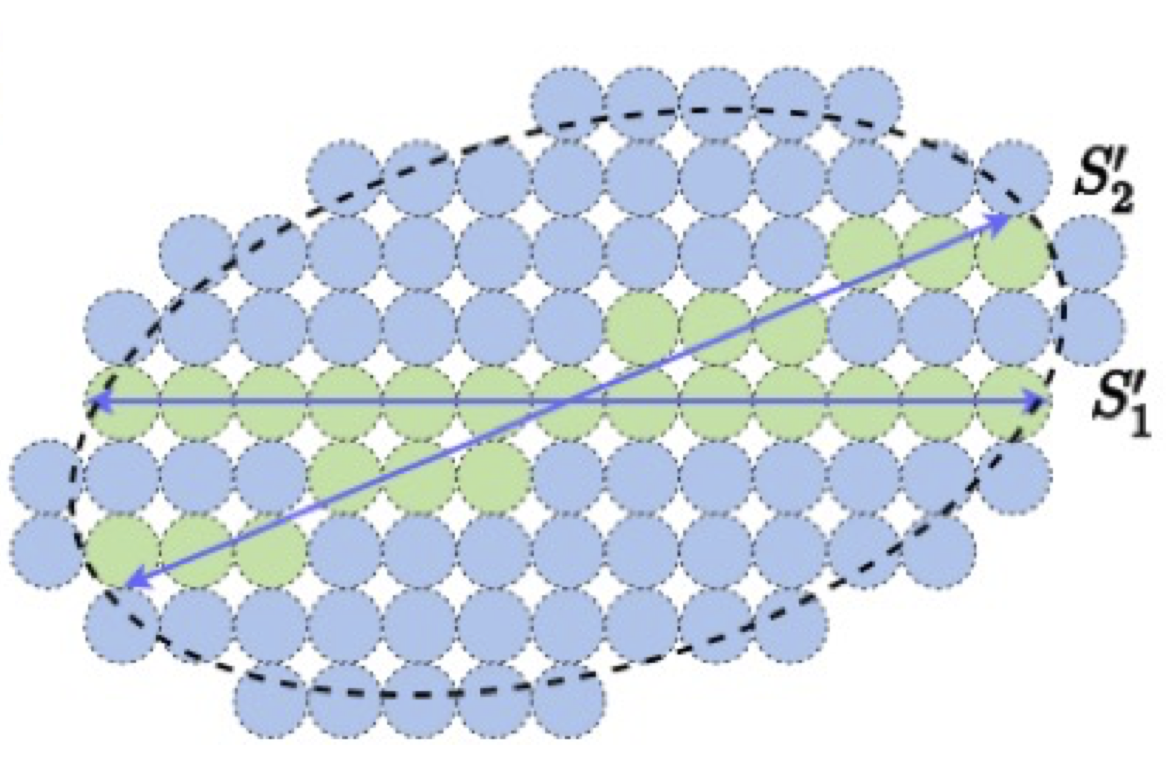
\includegraphics[width=0.5\linewidth]{\toplevelprefix/chapters/chapter1/figs/Coding-schemes.png}
    \caption{Comparație între două scheme de codare. Imaginați-vă că distribuția adevărată a datelor este în jurul celor două linii cu săgeți. Se pot codifica eșantioanele din cele două linii cu o carte de coduri constând din toate bilele albastre; se pot codifica și eșantioanele cu o carte de coduri constând doar din bilele verzi. Evident, a doua schemă de codare va duce la o lungime/rată de codare mult mai mică, sub rezerva aceleiași precizii.}
    \label{fig:coding-schemes}
\end{figure}


Apoi complexitatea funcției de predicție $f$ poate fi evaluată ca lungimea medie de codare a tuturor secvențelor, cunoscută sub numele de rata de codare:\footnote{Se poate face acest lucru mai precis luând $R(f\mid \mathcal{E})$ să fie lungimea așteptată de codare pentru toate segmentele de lungime $D$. }
\begin{equation}
   R(f \mid \mathcal E) = \mathbb{E}[L(\mathcal{E}(S))] \approx \frac{1}{N}\sum_{i=1}^N L(\mathcal{E}(S_i)).
   \label{eqn:coding-rate}
\end{equation}
Evident, măsura ratei de codare se va schimba dacă se folosește o schemă de codare diferită (sau o carte de coduri). În practică, cu cât cunoaștem mai bine structura cu dimensiuni reduse în jurul căreia sunt distribuite segmentele, cu atât o carte de coduri mai eficientă putem proiecta, ca exemplul arătat în Figura \ref{fig:coding-schemes}. Cititorii atenți ar fi putut recunoaște că, conceptual, procesul de îndepărtare a zgomotului ilustrat în Figura \ref{fig:diffusion} seamănă foarte mult cu trecerea de la schema de codare cu bilele albastre la cea cu cele verzi.


Având două scheme de codare $\mathcal{E}_1$ și $\mathcal{E}_2$ pentru segmente, dacă diferența în ratele de codare este pozitivă:
\begin{equation}
   R(f \mid \mathcal E_1) -  R(f \mid \mathcal E_2) > 0,
\end{equation}
putem spune că schema de codare $\mathcal{E}_2$ este mai bună. Această diferență poate fi văzută ca o măsură a cât de multă informație are $\mathcal{E}_2$ peste $\mathcal{E}_1$ despre distribuția datelor. Într-o mare măsură, obiectivul învățării $f$ este echivalent cu găsirea celei mai eficiente scheme de codare care minimizează rata de codare:
\begin{equation}
   \min_{\mathcal{E}} R(f \mid \mathcal E).
\end{equation}
După cum vom vedea în Capitolul \ref{ch:compression}, rata minimă realizabilă este strâns legată de noțiunea de entropie $H(S)$ \eqref{eqn:entropy-definition}.


\begin{remark}\label{rem:computable-complexity}
    {Perspectiva măsurării complexității datelor cu scheme de codare explicite a motivat mai multe obiective de învățare care au fost propuse pentru a revizui complexitatea Kolmogorov pentru o mai bună calculabilitate \cite{WallaceC1999}, inclusiv lungimea minimă a mesajului (MML) propusă mai târziu în 1968 \cite{WallaceC1968} și lungimea minimă de descriere (MDL) în 1978 \cite{Rissanen-1978,HansenM2001}. Aceste obiective numără în mod normal lungimea de codare pentru schema de codare $\mathcal{E}$ însăși (inclusiv cartea sa de coduri) în plus față de datele $S$ de interes: $L(\mathcal E(S)) + L(\mathcal E)$. Cu toate acestea, dacă obiectivul este să înveți o carte de coduri de dimensiune finită și să o aplici unui număr mare de secvențe, costul amortizat al cărții de coduri poate fi ignorat deoarece $$\frac{1}{N}\Big( L(\mathcal{E}) + \sum_{i=1}^N L(\mathcal{E}(S_i))\Big) \approx \frac{1}{N}\sum_{i=1}^N L(\mathcal{E}(S_i))$$ pe măsură ce $N$ devine mare.}
\end{remark}

Din nou, se poate vedea schema de codare optimă rezultată ca cea care obține cea mai bună compresie a datelor observate. În general, comparativ cu complexitatea Kolmogorov, lungimea de codare dată de orice schemă de codare va fi întotdeauna mai mare:
\begin{equation}
    K(S) < L( \mathcal E(S)).
\end{equation}
Prin urmare, minimizarea ratei/lungimii de codare este în esență minimizarea unei limite superioare a complexității Kolmogorov altfel necalculabile.

\subsection{Învățarea Reprezentărilor Informative}
Notați că dacă obiectivul ar fi pur și simplu să comprimăm datele date doar de dragul compresiei, atunci în teorie codurile optime care se apropie de complexitatea Kolmogorov ar deveni aproape aleatorii sau fără structură \cite{Chaitin-1966}.\footnote{Deoarece orice coduri cu structuri pot fi comprimate în continuare.} Cu toate acestea, adevăratul nostru scop de a învăța funcția predictivă $f$ este să o folosim în mod repetat cu ușurință în predicții viitoare. Prin urmare, în timp ce compresia ne permite să identificăm distribuția cu dimensiuni reduse în date, am dori să codificăm distribuția într-un mod {\em structurat și organizat}, astfel încât reprezentarea rezultată să fie foarte informativă și eficientă de utilizat.\footnote{De exemplu, pentru a eșantiona distribuția în condiții diferite.} Figura \ref{fig:expansion} arată un exemplu care explică intuitiv de ce o astfel de transformare este dorită.

\begin{figure}
    \centering
    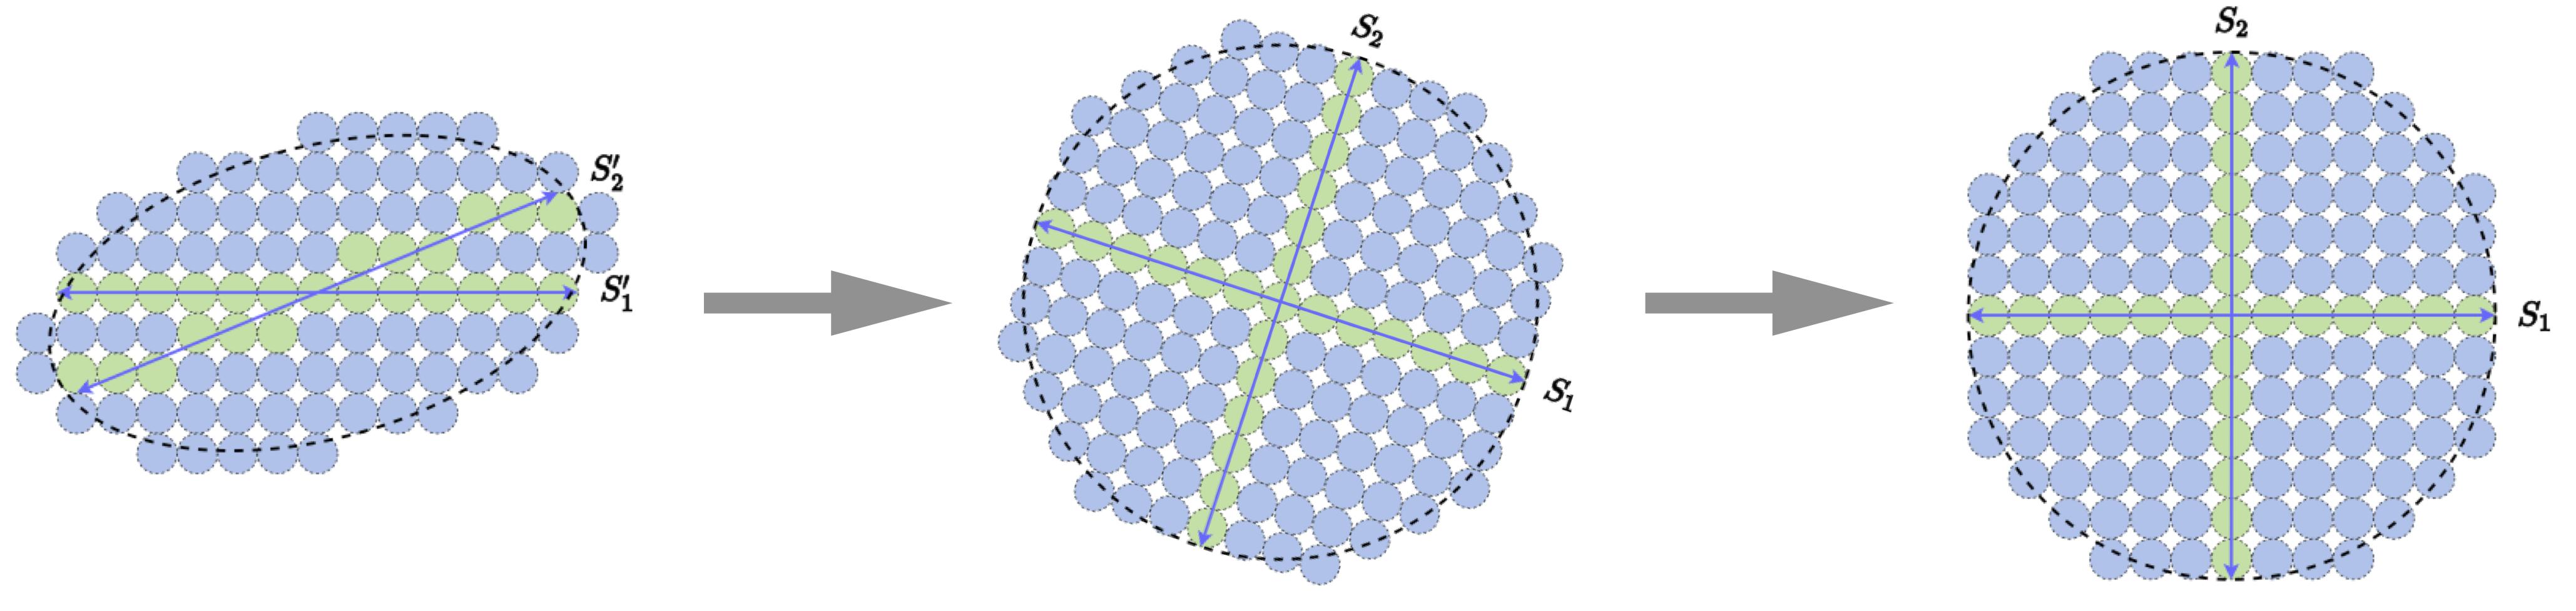
\includegraphics[width=0.98\linewidth]{\toplevelprefix/chapters/chapter1/figs/coding-transform.png}
    \caption{Transformarea distribuției de date cu dimensiuni reduse identificate într-o reprezentare mai informativă și structurată.}
    \label{fig:expansion}
\end{figure}
După cum vom arăta în Capitolul \ref{ch:compression}, aceste structuri dorite în reprezentarea finală pot fi promovate precis prin alegerea unei măsuri naturale de {\em câștig de informație} bazată pe ratele de codare ale schemelor de codare alese. După cum vedem în această carte, o astfel de abordare de codare explicită și constructivă oferă un cadru computațional puternic pentru învățarea reprezentărilor bune ale structurilor cu dimensiuni reduse pentru datele din lumea reală, deoarece în multe cazuri de importanță practică, funcția de lungime a codării poate fi calculată eficient sau aproximată cu acuratețe. În unele cazuri benigne, putem obține chiar formule în formă închisă, de exemplu, subspațiu și gaussiană (vezi Capitolul \ref{ch:compression}).

În plus, un astfel de cadru computațional duce la o abordare principială care dezvăluie în mod natural rolul pe care rețelele profunde îl joacă în acest proces de învățare. După cum vom deriva sistematic în Capitolul \ref{ch:representation}, straturile unei rețele profunde încearcă să efectueze operații care optimizează funcția obiectiv de interes într-o manieră incrementală. Din această perspectivă, rolul rețelelor profunde poate fi interpretat precis ca emularea unui anumit algoritm de optimizare iterativă, să zicem coborârea pe gradient, pentru a optimiza obiectivul câștigului de informație. Straturile arhitecturilor profunde rezultate pot fi înzestrate cu interpretare statistică și geometrică precisă, și anume efectuarea operațiilor incrementale de codare și decodare compresivă. Ca rezultat, rețelele profunde derivate devin „cutii albe" transparente care sunt complet explicabile matematic.










\subsection{Învățarea Reprezentărilor Consistente}

\label{sec:consistency}
Pentru a rezuma discuțiile noastre de până acum, să notăm datele ca:
\begin{equation}
    \boldsymbol{X} = \{S_1, S_2, \ldots, S_i, \ldots, S_N\} \subset \mathbb{R}^D,
\end{equation}
și fie $\boldsymbol{Z} = \mathcal{E}(\X)$ codurile lui $\X$ printr-un anumit codificator $\mathcal{E}$:
\begin{equation}
    \X  \xrightarrow{\hspace{2mm} \mathcal{E}\hspace{2mm}} \Z.
    \label{eqn:open-loop}
\end{equation}
În contextul învățării automate, $\Z$ este adesea numit „caracteristici" sau „reprezentare latentă". Notați că fără a cunoaște distribuția de bază a lui $\X$, nu știm care codificator $\mathcal{E}$ ar trebui să fie cel care poate păstra cele mai utile informații despre distribuția lui $\X$. În practică, oamenii încep adesea cu încercarea unei anumite scheme de codare compacte care servește bine pentru o sarcină specifică. În special, ar încerca să învețe un codificator care optimizează o anumită măsură (empirică) de parcimonie pentru reprezentarea învățată:
\begin{equation}
    \min \rho(\Z).
\end{equation}

\begin{example}
De exemplu, clasificarea imaginilor este un astfel de caz: atribuim toate imaginile din aceeași clasă unui singur cod și imaginile din clase diferite la coduri diferite, să zicem vectori „one-hot":
\begin{equation}
  \x \mapsto \z \in \{  [1, 0, 0, \ldots , 0, 0], \;  [0, 1, 0 \ldots, 0, 0], \; \ldots, \;  [0,0,0, \ldots, 0, 1].\}
  \label{eqn:class-labels}
\end{equation}
Acum, un clasificator $f(\cdot)$ poate fi modelat ca o funcție care prezice probabilitatea ca un $\x$ dat să aparțină fiecăreia dintre cele $k$ clase: $\hat{\z} = f(\x) \in \mathbb{R}^K$. Apoi „bunătatea" unui clasificator poate fi măsurată prin așa-numita {\em entropie încrucișată}:\footnote{Entropia încrucișată poate fi văzută ca o măsură de distanță între distribuția adevărului de bază a lui $\z$ și cea a predicției $\hat\z$. Poate fi văzută și ca lungimea așteptată de codare a lui $\z$ dacă folosim cartea de coduri optimă pentru $\hat \z$ pentru a codifica $\z$. Entropia încrucișată atinge minimul când $\z$ și $\hat \z$ au aceeași distribuție.}
\begin{equation}
    L(\hat{\z}, \z) = \sum_{k=1}^K - z_k \log \hat{z}_k,
\end{equation}
unde $z_k$ indică a $k$-a intrare a vectorului $\z$. După cum a indicat practica timpurie a rețelelor profunde \cite{krizhevsky2012imagenet}, dacă sunt date suficiente date, o astfel de schemă de codare poate fi adesea reprezentată de o rețea profundă și învățată într-o manieră de la cap la coadă prin optimizarea entropiei încrucișate.
\end{example}

Pierderea entropiei încrucișate $L(\hat \z, \z)$ poate fi văzută ca o măsură specială de parcimonie $\rho(\z)$ asociată cu o familie particulară de scheme de codare care sunt potrivite pentru clasificare. Cu toate acestea, o astfel de codare este evident {\em foarte cu pierderi}. $\z$ învățat nu conține nicio altă informație despre $\x$ cu excepția tipului său de clasă. De exemplu, prin atribuirea unei imagini cu (un cod reprezentând) eticheta de clasă „măr", nu mai știm ce tip specific de măr se află în imaginea originală doar din etichetă.

Desigur, cealaltă extremă este să cerem ca schema de codare să fie {\em fără pierderi}. Adică, există o mapare unu-la-unu între $\x$ și codul său $\z$. Cu toate acestea, după cum vom vedea în \Cref{ch:compression}, codarea fără pierderi (sau compresia) este impracticabilă decât dacă $\x$ este discret. Pentru o variabilă aleatorie continuă, putem lua în considerare doar scheme de codare cu pierderi, astfel încât lungimea de codare pentru date să poată fi finită. Adică, codificăm datele doar până la o anumită precizie prescrisă. După cum vom elabora mai mult în \Cref{ch:compression}, codarea cu pierderi nu este doar o alegere practică; joacă un rol fundamental în a face posibilă învățarea distribuției continue de bază din eșantioane finite ale distribuției.

Pentru multe scopuri de învățare, dorim ca caracteristica $\z$, deși {\em cu pierderi}, să păstreze mai multe informații despre $\x$ decât doar tipul său de clasă. În această carte, vom introduce o măsură mai generală de parcimonie bazată pe lungimea/rata de codare asociată cu o familie mai generală de scheme de codare -- codarea cu un amestec de subspații sau gaussiene. Această familie are capacitatea de a aproxima îndeaproape distribuții arbitrare din lumea reală până la o anumită precizie. După cum vom vedea în \Cref{ch:compression} și \Cref{ch:representation}, o astfel de măsură nu numai că va păstra majoritatea informațiilor despre distribuția lui $\X$, dar va promova și anumite structuri geometrice și statistice frumoase dorite pentru reprezentarea învățată $\Z$.


\paragraph{Autocodare Bidirecțională pentru Consistență.}
Într-un context de învățare mai larg, obiectivul principal al unei scheme de codare compresive $\mathcal{E}$ este să identifice structurile cu dimensiuni reduse din datele $\X$, astfel încât acestea să poată fi folosite pentru a prezice lucruri în spațiul original al datelor. Aceasta necesită ca schema de codare învățată $\mathcal{E}$ să permită o schemă de decodare eficientă, notată ca $\mathcal D$. Aceasta mapează $\Z$, adesea cunoscută ca reprezentare latentă, înapoi la spațiul datelor:
\begin{equation}
    \X   \xrightarrow{\hspace{2mm} \mathcal{E}\hspace{2mm}} \Z  \xrightarrow{\hspace{2mm} \mathcal{D} \hspace{2mm}} \hat \X.
       \label{eqn:auto-encoding}
\end{equation}
În general, numim o astfel de pereche de codare și decodare $(\mathcal{E}, \mathcal{D})$ o {\em autocodare}. \Cref{fig:autoencoder} ilustrează procesul unui astfel de autocodor.
\begin{figure}
    \centering
    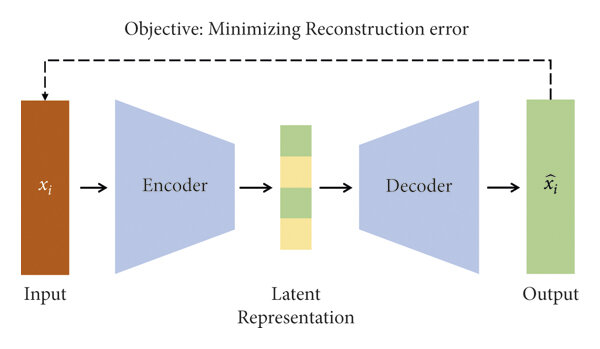
\includegraphics[width=0.7\linewidth]{\toplevelprefix/chapters/chapter1/figs/Autoencoder.jpg}
    \caption{Ilustrarea arhitecturii unui autocodor.}
    \label{fig:autoencoder}
\end{figure}


În general, am prefera ca decodarea să fie aproximativ un „invers" al codării, astfel încât datele (distribuția) $\hat \X$ decodate din $\Z$ să fie similare cu datele (distribuția) originale $\X$ într-o anumită măsură.\footnote{Vom face mai precis ce înțelegem prin a fi similar mai târziu.} Dacă da, am putea recupera sau prezice din $\Z$ ce se întâmplă în spațiul original al datelor. În acest caz, spunem că perechea $(\mathcal{E}, \mathcal{D})$ oferă o autocodare {\em consistentă}. Pentru majoritatea scopurilor practice, nu numai că avem nevoie ca o astfel de decodare să existe, dar să poată fi și realizată eficient și implementată fizic. De exemplu, dacă $\x$ este o variabilă cu valori reale, este necesară cuantificarea pentru ca orice schemă de decodare să fie realizabilă pe o mașină cu stare finită, așa cum vom explica mai mult în Capitolul \ref{ch:compression}. Prin urmare, în general, ar trebui să ne așteptăm ca schemele de codare și decodare realizabile să fie neapărat cu pierderi. O întrebare centrală este cum să învățăm o reprezentare compactă (cu pierderi) $\Z$ astfel încât să poată fi folosită pentru a prezice bine $\X$.

În general vorbind, după cum vom vedea, atât codificatorul, cât și decodificatorul ar putea fi modelate și realizate de rețele profunde și învățate prin rezolvarea unei probleme de optimizare de următoarea formă:
\begin{equation}
   \min \, d( \X, \hat \X) + \rho(\Z),
   \label{eqn:auto-encoding-objective}
\end{equation}
unde $d(\cdot, \cdot)$ este o anumită funcție de distanță care promovează similaritatea între $\X$ și $\hat \X$\footnote{Fie similar pe eșantion, fie similar pe distribuție, în funcție de alegerea funcției de distanță $d$.} și $\rho(\Z)$ este o anumită măsură care promovează parcimonia și bogăția informațională a lui $\Z$. Analiza clasică a componentelor principale (PCA) \cite{JolliffeI2002} este un exemplu tipic de autocodare consistentă, pe care o vom studia în detaliu în Capitolul \ref{ch:classic}, ca precursor al structurilor mai generale cu dimensiuni reduse. În Capitolul \ref{ch:autoencoding}, vom studia cum să învățăm autocodare consistentă pentru distribuții generale (să zicem neliniare) cu dimensiuni reduse.


\subsection{Învățarea Reprezentărilor Auto-Consistente}
Notați că în obiectivul de autocodare de mai sus, trebuie să evaluăm cât de aproape sau consistente sunt datele decodate $\hat \X$ cu originalul $\X$. Acest lucru necesită adesea o anumită supraveghere externă sau cunoștințe despre ce măsură de similaritate să folosim. Calcularea similarității între $\hat \X$ și $\X$ poate fi foarte costisitoare, dacă nu în întregime imposibilă sau intractabilă.\footnote{Să zicem că cineva vrea să minimizeze o anumită distanță distribuțională între cele două.} Notați că în natură, animalele sunt capabile să învețe toate de la sine fără a compara estimarea lor $\hat \X$ cu adevărul de bază $\X$ în spațiul datelor. De obicei, nici măcar nu au acea opțiune.

Atunci cum este capabil un sistem să învețe autonom fără supraveghere externă sau comparație? Cum pot să știe că $\hat \X$ este consistent cu $\X$ chiar fără a le compara direct? Aceasta duce la ideea de „închidere a buclei". După cum se dovedește, în condiții blânde pe care le vom face precise în Capitolul \ref{ch:closed-loop}, pentru a asigura că $\X$ și $\hat \X$ sunt consistente, trebuie doar să codificăm $\hat \X$ ca $\hat \Z$ și să verificăm dacă $\Z$ și $\hat \Z$ sunt consistente. Numim această noțiune de consistență {\em auto-consistență}, care poate fi ilustrată prin următoarea diagramă:
\begin{equation}
    \X   \xrightarrow{\hspace{2mm} \mathcal{E}\hspace{2mm}} \Z  \xrightarrow{\hspace{2mm} \mathcal{D} \hspace{2mm}} \hat \X \xrightarrow{\hspace{2mm} \mathcal{E}\hspace{2mm}} \hat \Z,
    \label{eqn:closed-loop}
\end{equation}
Ne referim la acest proces ca o {\em transcriere în buclă închisă},\footnote{Inspirat de procesul de transcriere între ADN și ARN sau alte proteine.} care este ilustrat în Figura \ref{fig:closed-loop}.

\begin{figure}[t]
    \centering
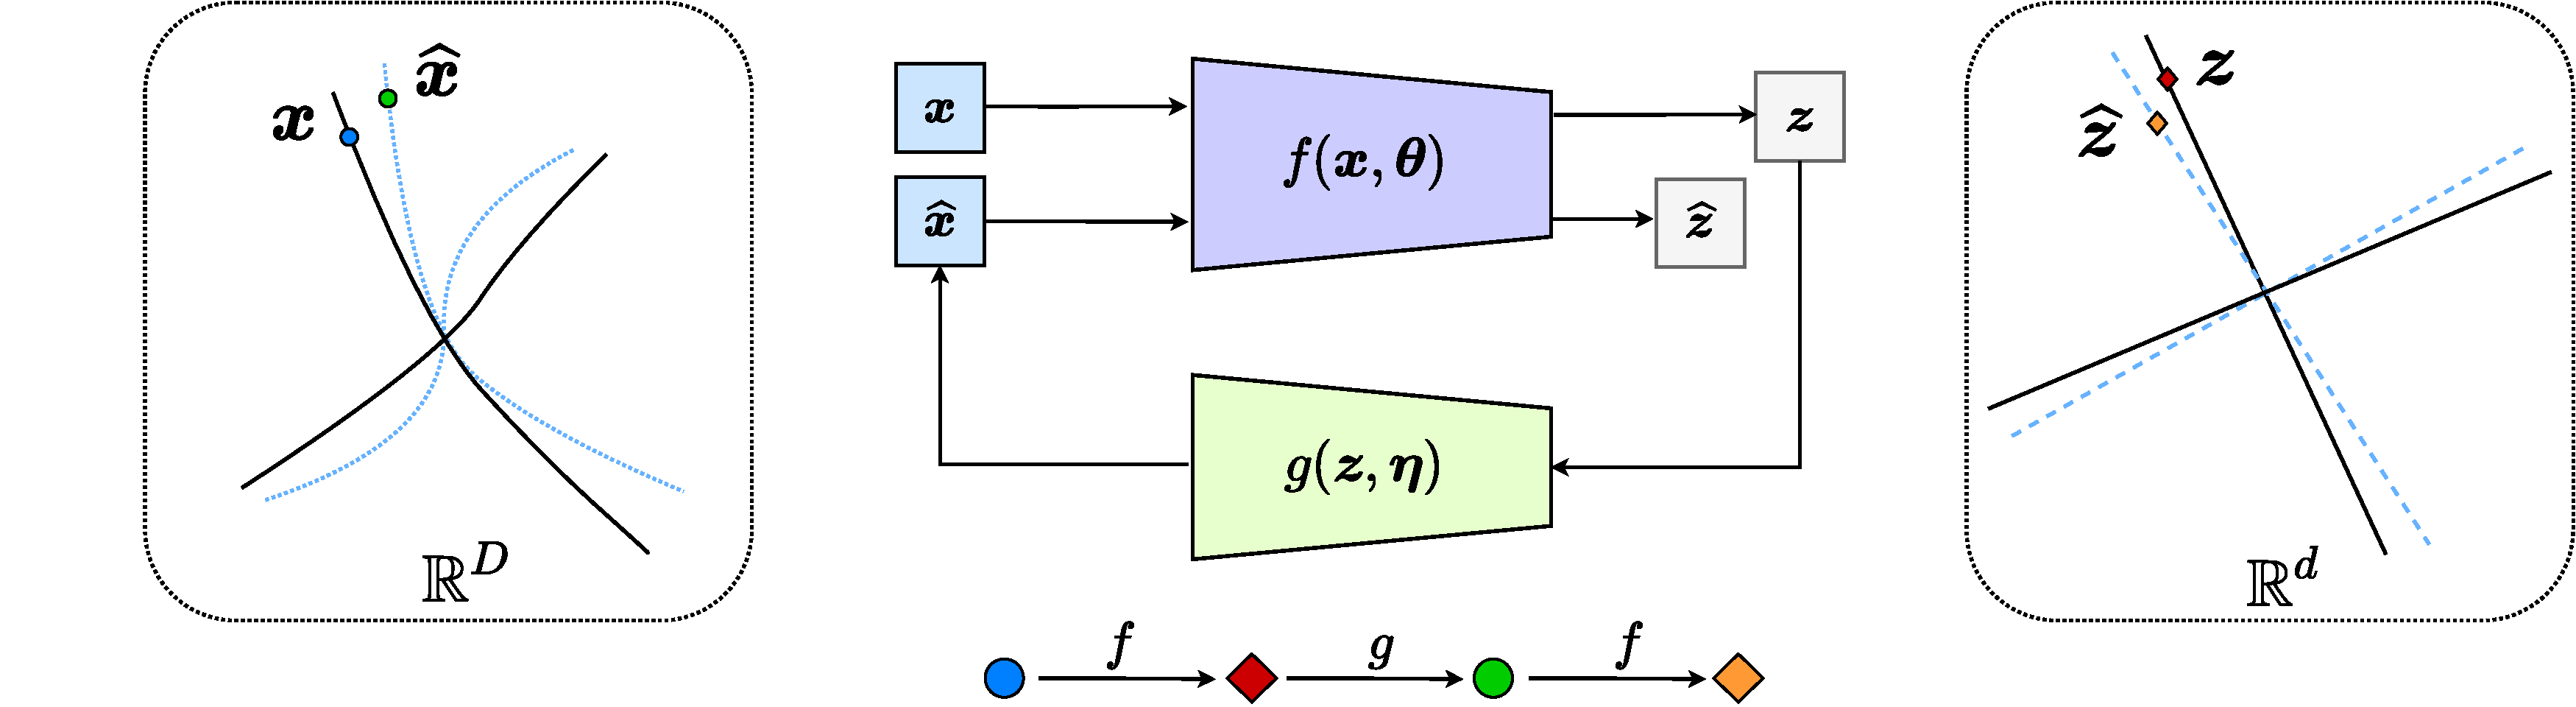
\includegraphics[width=0.9\linewidth]{\toplevelprefix/chapters/chapter1/figs/diagrams_redu_gan_2.pdf}
\caption{Ilustrarea unei transcrieri în buclă închisă. Aici folosim o mapare $f$ pentru a reprezenta codificatorul $\mathcal{E}$ și $g$ pentru a reprezenta decodificatorul $\mathcal{D}$.}  \label{fig:closed-loop}
\end{figure}

Este probabil adevărat că orice ființă inteligentă autonomă trebuie doar să învețe o reprezentare auto-consistentă $\Z$ a datelor observate $\X$, deoarece verificarea consistenței în spațiul original al datelor (adesea însemnând în lumea externă) este fie prea costisitoare, fie chiar nu este fezabilă fizic. Formularea în buclă închisă permite să învățăm o codare optimă $f(\cdot, \theta)$ și decodare $g(\cdot, \eta)$ printr-un joc minmax care depinde doar de caracteristica internă (învățată) $\Z$:
\begin{equation}
\max_{\theta}\min_{\eta} \ell( \Z, \hat \Z) + \rho(\Z),
   \label{eqn:closed-loop-objective}
\end{equation}
unde $\ell( \Z, \hat \Z)$ este o funcție de pierdere bazată pe ratele de codare ale caracteristicilor $\Z$ și $\hat \Z$, care, după cum vom vedea, poate fi mult mai ușor de calculat. Aici din nou, $\rho(\Z)$ este o anumită măsură care promovează parcimonia și bogăția informațională a lui $\Z$. Oarecum surprinzător, după cum vom vedea în Capitolul \ref{ch:closed-loop}, în condiții destul de blânde, cum ar fi $\X$ fiind suficient de cu dimensiuni reduse, auto-consistența între $(\Z, \hat \Z)$ implică consistență în $(\X, \hat \X)$! În plus, vom vedea și că un sistem în buclă închisă ne va permite să învățăm distribuția într-o manieră {\em continuă și incrementală},\footnote{Adică să învățăm cu o clasă la un moment dat sau chiar un eșantion la un moment dat.} fără a suferi de probleme precum uitarea catastrofală asociată cu modelele în buclă deschisă.

\section{Punți între Teorie și Practică pentru Inteligența Mașinilor}
Până acum, am introdus trei cadre conexe pentru învățarea unei reprezentări compacte și structurate $\Z$ pentru o distribuție de date dată $\X$:
\begin{itemize}
\item Codarea deschisă \eqref{eqn:open-loop};
\item Autocodarea bidirecțională \eqref{eqn:auto-encoding};
\item Transcrierea în buclă închisă \eqref{eqn:closed-loop}.
\end{itemize}
În această carte, vom studia sistematic toate cele trei cadre, unul după altul:
\begin{equation}
    \mbox{\textbf{deschis}} \; \Longrightarrow \;
    \mbox{\textbf{bidirecțional}} \;  \Longrightarrow \; \mbox{\textbf{buclă închisă}},
\end{equation}
în Capitolul \ref{ch:representation}, Secțiunea \ref{sec:consistent-representation} și Secțiunea \ref{sec:self-consistency} din Capitolul \ref{ch:autoencoding}, respectiv.

În ultimii câțiva ani, au fost propuse și dezvoltate multe cadre teoretice pentru a ajuta la înțelegerea rețelelor profunde. Cu toate acestea, multe nu au putut oferi soluții scalabile care să egaleze performanța metodelor empirice pe date și sarcini din lumea reală. Multe teorii nu oferă îndrumări utile despre cum să îmbunătățim în continuare practica. Capitolele \ref{ch:conditional-inference} și \ref{ch:applications} vor arăta cum cadrul prezentat în această carte poate ajuta la reducerea decalajului dintre teorie și practică. Capitolul \ref{ch:conditional-inference} va arăta cum să folosim distribuția învățată și reprezentarea sa pentru a efectua inferență (Bayesiană) pentru aproape toate sarcinile practice care depind de generarea, estimarea și predicția (condiționată). Capitolul \ref{ch:applications} va oferi dovezi experimentale convingătoare că rețelele și sistemele proiectate din primele principii pot obține performanțe competitive și potențial mai bune pe o varietate de sarcini, cum ar fi învățarea reprezentării vizuale, clasificarea imaginilor, completarea imaginilor, segmentarea și generarea de text.


\paragraph{Înapoi la Inteligență.}
După cum am menționat la început, o sarcină comună și fundamentală a oricărei ființe inteligente este să învețe informații previzibile din datele sale percepute. Acum am înțeles puțin despre natura computațională a acestei sarcini și cineva ar trebui să realizeze că acesta este un proces fără sfârșit, din următoarele motive:
\begin{itemize}
    \item Cunoștințele învățate până acum din date, să zicem prin schemele de codare și decodare, este puțin probabil să fie corecte sau optime. Inteligența ar trebui să aibă capacitatea de a se îmbunătăți dacă există încă erori în prezicerea noilor observații.
    \item Datele observate până acum nu acoperă încă toate informațiile previzibile. Inteligența ar trebui să poată recunoaște că cunoștințele actuale sunt inadecvate și să aibă capacitatea de a învăța și dobândi informații noi ori de câte ori sunt disponibile.
\end{itemize}

Prin urmare, inteligența {\em nu} este despre simpla colectare a tuturor datelor în avans și antrenarea unui model pentru a memoriza toate informațiile previzibile din date. În schimb, este despre a fi echipat cu mecanisme computaționale care pot îmbunătăți constant cunoștințele actuale și pot dobândi informații noi când sunt disponibile și necesare. Adică, o caracteristică fundamentală a oricărei ființe sau sistem inteligent\footnote{Un animal, o ființă umană, un robot inteligent, comunitatea științifică și chiar întreaga civilizație.} este {\em a putea să se îmbunătățească continuu sau să câștige informații (sau cunoștințe) pe cont propriu}. Conceptual, putem ilustra simbolic relația dintre inteligență și informație (sau cunoaștere) după cum urmează:
\begin{equation}
\operatorname{Inteligență}(t) = \odv*{\operatorname{Informație}}{t}(t), \qquad
\operatorname{Informație}(t)  = \int_0^t \operatorname{Inteligență}(s) \odif{s}.
\end{equation}
Credem că cadrul în buclă închisă este un mecanism universal care permite auto-îmbunătățirea și auto-învățarea, prin feedback\footnote{Întărirea poate fi văzută ca o formă primitivă de feedback, să zicem selecția naturală de către natură.} sau joc\footnote{Investigațiile științifice pot fi văzute ca o formă cea mai avansată de joc, prin formularea și verificarea ipotezelor.}. Toate ființele sau sistemele inteligente din natură utilizează mecanisme în buclă închisă pentru învățare la toate nivelurile și pe toate scările. Omniprezența sa a inspirat studii timpurii care au încercat să modeleze și să emuleze inteligența prin mașini și calculatoare, în special mișcarea Cibernetică inițiată de Norbert Wiener în anii 1940.

Sperăm că această carte va ajuta oamenii să înțeleagă mai bine obiectivele, principiile și mecanismele computaționale din spatele inteligenței. Servește ca o fundație pentru studiul ulterior al inteligenței umane de nivel superior, adevărata „inteligență artificială", în viitor, pentru care vom prezenta câteva probleme deschise semnificative în aceste noi direcții la sfârșitul cărții în Capitolul \ref{ch:future}.

\end{document}
